\documentclass[12pt,a4paper]{article}
 
\usepackage{float}
%für feststellen der figures und tables [H] dranschreiben
\usepackage{units}
%wird so benutzt: 
%\unit[value/Zahl]{dimension/Einheit} oder 
%\unitfrac[value/Zahl]{dimension/Einheit num/Zähler}{dimension/Einheit denum/Nenner} oder
%\nicefrac[fontcommand/Schriftart]{dimension/Einheit num/Zähler}{dimension/Einheit denum/Nenner}
\usepackage[left=2cm,right=2cm,top=2cm,bottom=2cm]{geometry}
\usepackage[utf8]{inputenc}
\usepackage[T1]{fontenc}
\usepackage{lmodern}
\usepackage[ngerman]{babel}
\usepackage{amsmath}
\usepackage{graphicx}

\usepackage{caption}
\usepackage{subcaption}
 
\title{Versuch EP1}
\author{Frederik Strothmann, Henrik Jürgens}
\date{\today}
%niemals zwei überschriften direkt übereinander schreiben, also immer mindestens in einem satz was sinnvolles unter jede überschrift schreiben (bei den versuchen z.B. das versuchsziel) 
\begin{document}
%deckblatt erstellen.
\maketitle
\newpage
\tableofcontents
\newpage




\newpage\section{Einleitung}
%einleitung zu dem experiment.
%auf die einstellungen, die vor dem versuch gemacht werden, eingehen oder auf eine anleitung dazu verweisen.
%---------------------------------------------------------------------------------------------
%hinter der einleitung kann der allgemeine theoretische hintergrund in einer zusätzlichen section erklärt werden
Dieser Versuch beschäftigt sich mit den Übertragungseigenschaften verschiedener Kabel. Untersucht werden Bananenkabel, BNC-Kabel und Patchkabel.\newline
In den Aufbauten wird die Signalqualität der Kabel abhängig von der Einstellung des Funktionsgenerators (Sinus oder Rechteck), der Kabellänge und der Schaltung miteinder verglichen.\newline
Der sogenannte 'Kapazitätsbelag' (Kapazität zwischen Signal und Masseleitung) des BNC- und Patchkabels, welcher neben drei weiteren Kabelkonstanten (Selbstinduktivität der Leitung, Widerstand der Signalleitung, Leitwert der Isolation) bei der Beschreibung der Kabeleigenschaften eine wichtige Rolle spielt wird ebenfalls bestimmt. 


\section{Verwendete Materialien}
%(immer) eine skizze oder ein foto einfügen, die geräte/materialien !nummerieren! und z.b. eine legende dazu schreiben
%falls am anfang des versuches nicht klar ist, was alles verwendet wird, wenn möglich erst am ende ein großes foto von den verwendeten materialien machen!
%-------------------------------------------------------------------------------------------
%ab hier für jeden versuchsteil einzeln, falls noch materialien hinzugenommen wurden immer im versuchsaufbau erwähnen!
Verwendet wurden: 

\begin{itemize}
\item	Funktionsgenerator zum erzeugen der Signale

\item	Oszilloskop zur graphischen Darstellung der Signale

\item	Bananenkabel zur Signalübertragung

\item	Koaxialkabel zur Signalübertragung

\item	Patchkabel zur Signalübertragung

\item	Mikrofon zum Signalerzeugen

\item	Operationsverstärker zum verstärken des Mikrofonsignals

\item	T-Verbindungsstück zum anschließen zusätzlicher Kabel

\item	BNC-Bananenkabel Adapter

\item 	Verschiedene Widerstände/Potentiometer

\end{itemize}

\section{Versuchsteil 1}
Der erste Versuchsteil war nicht mit Messungen versehen, wodurch die Nummerierung bei Versuchsteil zwei anfängt.

\section{Signalausbreitung über einfache Kabel}
%kurz das ziel dieses versuchsteiles ansprechen, damit keine zwei überschriften direkt übereinander stehen!
%bei schwierigeren versuchen kann auch der theoretische hintergrund erläutert werden. (mit formeln, herleitungen und erklärungen)
Im zweitem Versuchsteil sollte die Störanfälligkeit von Signalen bei Übertragung mit Bananenkabeln überprüft werden. Dabei wurden drei verschiedene Übertragungsmöglichkeiten verwendet, Übertragung mit nur einem Bananenkabel, mit zwei Bananenkabeln und mit einem twisted-pair Kabel aus zwei Bananenkabeln.
\subsection{Versuchsaufbau}
%skizze zum versuchsaufbau (oder foto) einfügen,   es muss erklärt werden wie das ganze funktioniert und welche speziellen einstellungen verwendet wurden (z.b. welche knöpfe an den geräten für die messung verdreht wurden)

Der Versuchsaufbau teilt sich in drei Teile auf.

\subsubsection{2.1 Ein Bananenkabel und gemeinsame Masse}

Für die Signalübertragung mit nur einem Bananenkabel wurde der Aufbau aus Abbildung \ref{fig:2.1} verwendet.

\begin{figure}[H] 
  \centering
    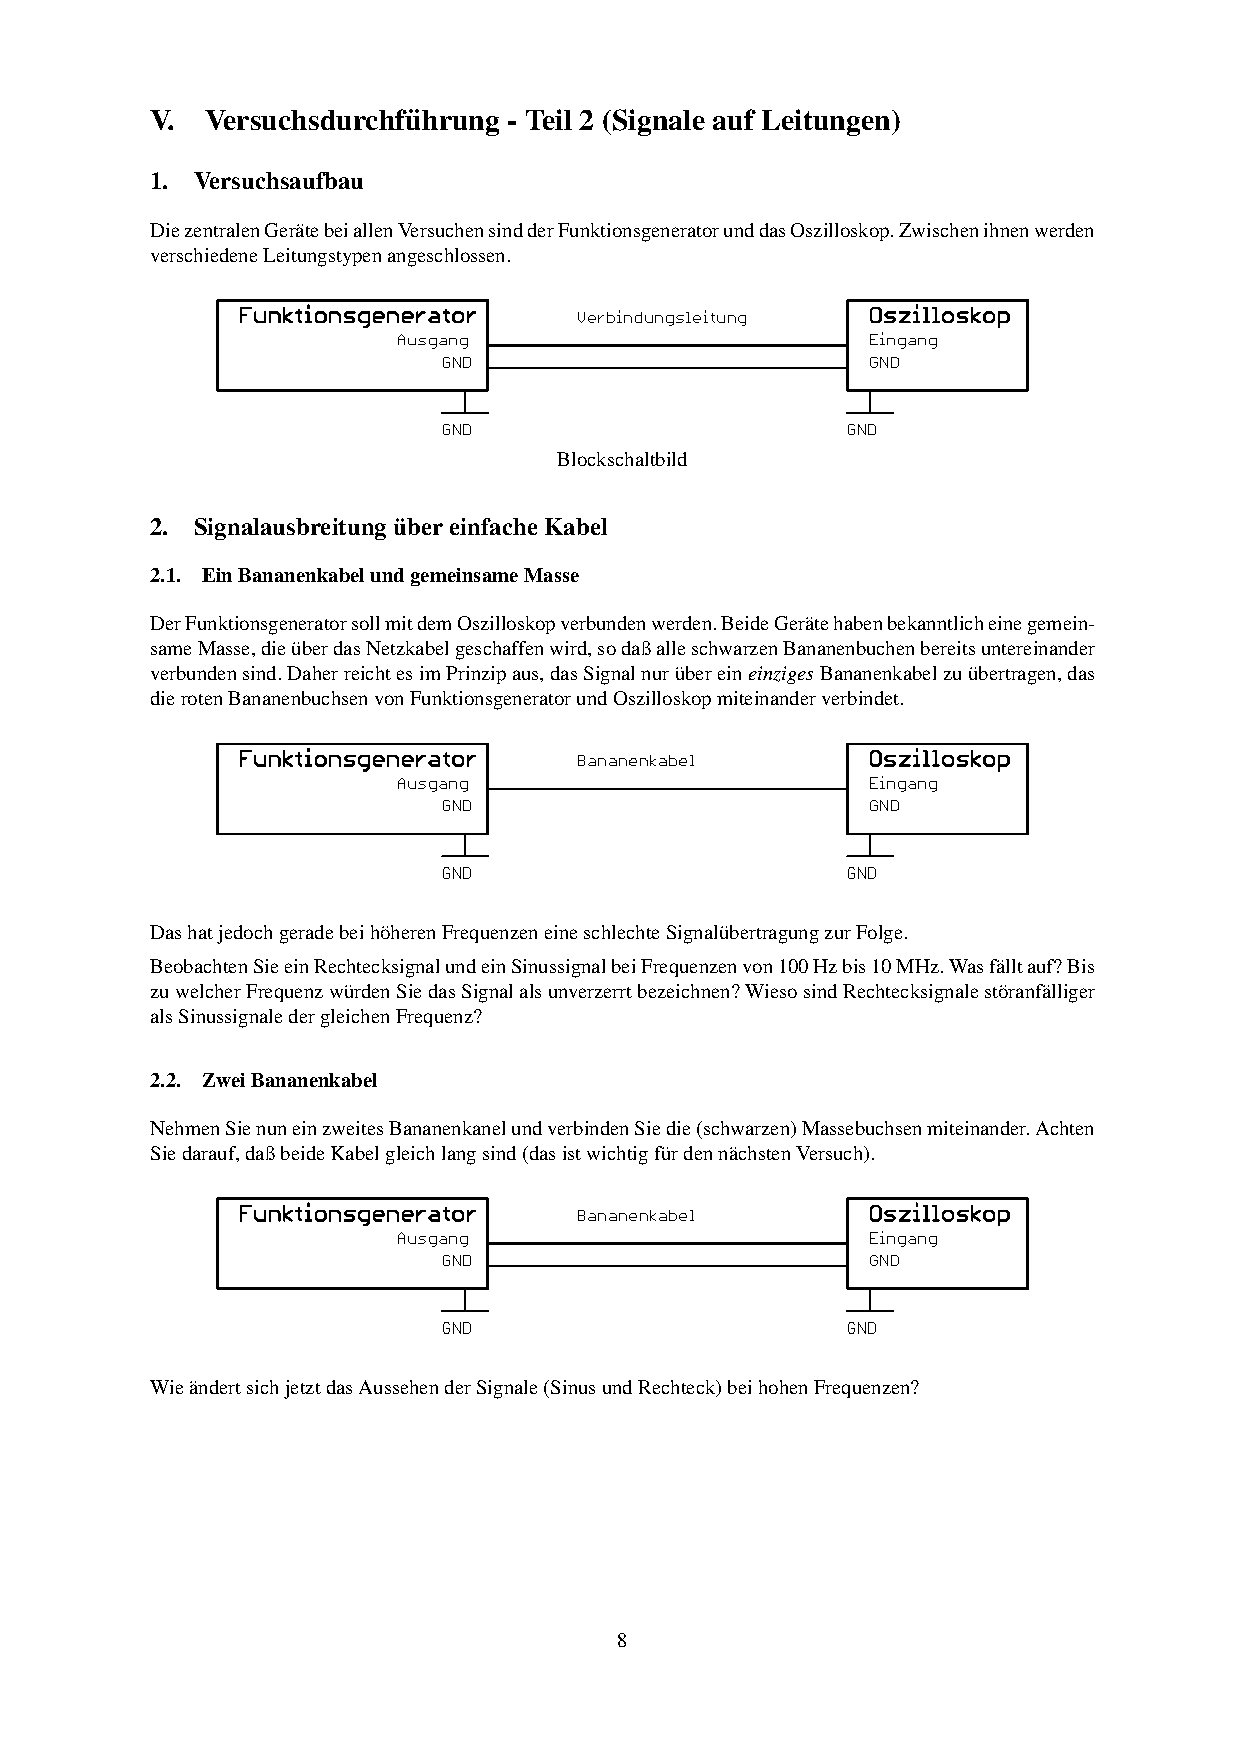
\includegraphics[trim = 10mm 142mm 10mm 125mm, clip, scale = 1]{2_0-2_2.pdf}
  	\caption[Schaltskizze einer Verbindung zwischen Funktionsgenerator und Oszilloskop, mit einem Bananenkabel]{Schaltskizze einer Verbindung zwischen Funktionsgenerator und Oszilloskop, mit einem Bananenkabel\footnotemark}
  \label{fig:2.1}
\end{figure}
\footnotetext{Abbildung entnommen von http://www.atlas.uni-wuppertal.de/$\sim$kind/ep1\_14.pdf Seite 8 am 19.10.2014}

\subsubsection{2.2 Zwei Bananenkabel}

Bei der Signalübertragung mit zwei Bananenkabeln wurde der Aufbau aus Abbildung \ref{fig:2.2} verwendet.

\begin{figure}[H] 
  \centering
    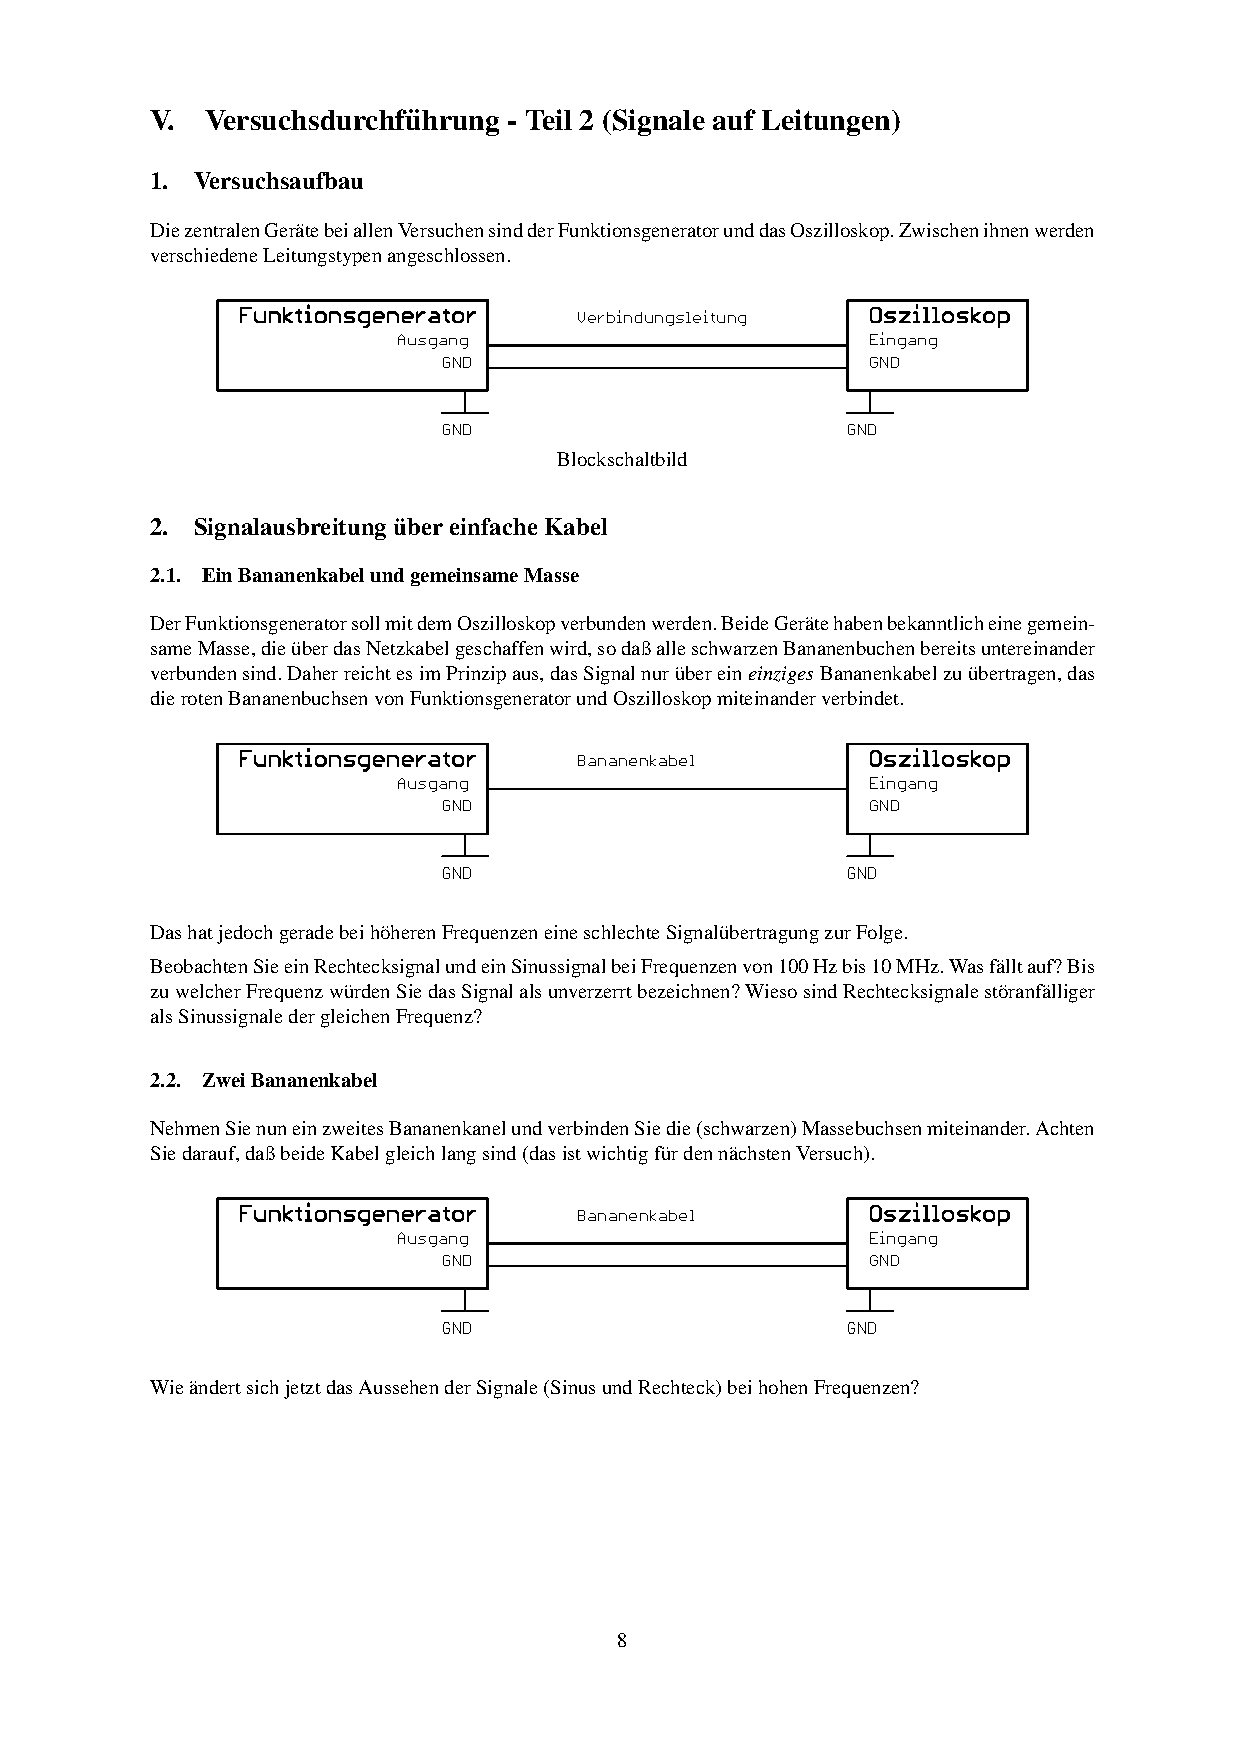
\includegraphics[trim = 10mm 70mm 10mm 200mm, clip, scale = 1]{2_0-2_2.pdf}
  	\caption[Schaltskizze einer Verbindung zwischen Funktionsgenerator und Oszilloskop, mit zwei Bananenkabeln]{Schaltskizze einer Verbindung zwischen Funktionsgenerator und Oszilloskop, mit zwei Bananenkabeln\footnotemark}
  \label{fig:2.2}
\end{figure}
\footnotetext{Abbildung entnommen von http://www.atlas.uni-wuppertal.de/$\sim$kind/ep1\_14.pdf Seite 8 am 19.10.2014}

\subsubsection{2.3 Zwei verdrillte Bananenkabel}

Für die Signalübertragung über ein twisted-pair Kabel wurden die Bananenkabel aus Abbildung \ref{fig:2.2} miteinander verdrillt.

\begin{figure}[H] 
  \centering
    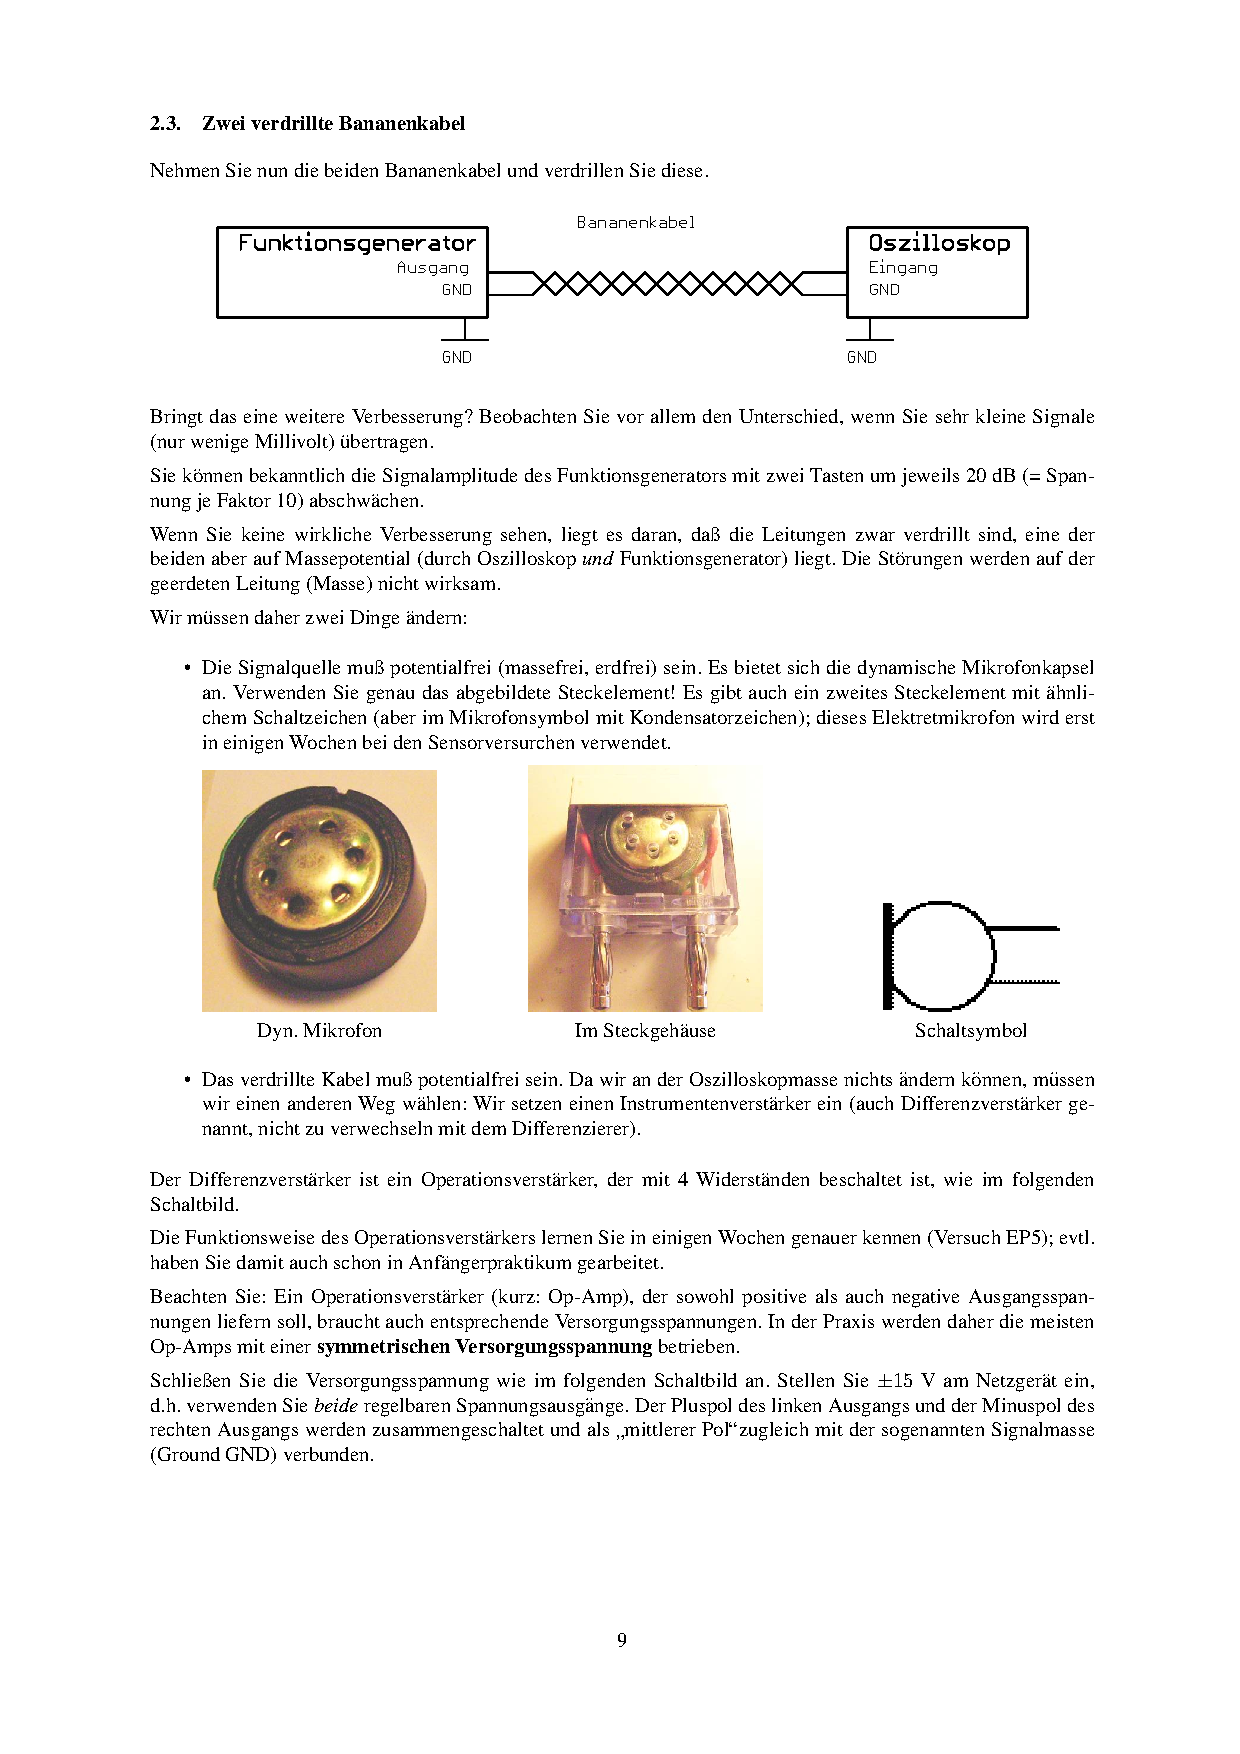
\includegraphics[trim = 10mm 230mm 10mm 32mm, clip, scale = 1]{2_3.pdf}
  	\caption[Schaltskizze einer Verbindung zwischen Funktionsgenerator und Oszilloskop, mit zwei verdrillten Bananenkabeln]{Schaltskizze einer Verbindung zwischen Funktionsgenerator und Oszilloskop, mit zwei verdrillten Bananenkabeln\footnotemark}
  \label{fig:2.3}
\end{figure}
\footnotetext{Abbildung entnommen von http://www.atlas.uni-wuppertal.de/$\sim$kind/ep1\_14.pdf Seite 9 am 19.10.2014}

Als alternative zu dem geerdetem Funktionsgenerator wird ein Mikrofon als Signalquelle verwendet. Das Signal wir über einen Operationsverstärker, siehe Abbildung \ref{fig:2.33} verstärkt, um das Signal auf dem Oszilloskop sichtbar zu machen.

\begin{figure}[H] 
  \centering
    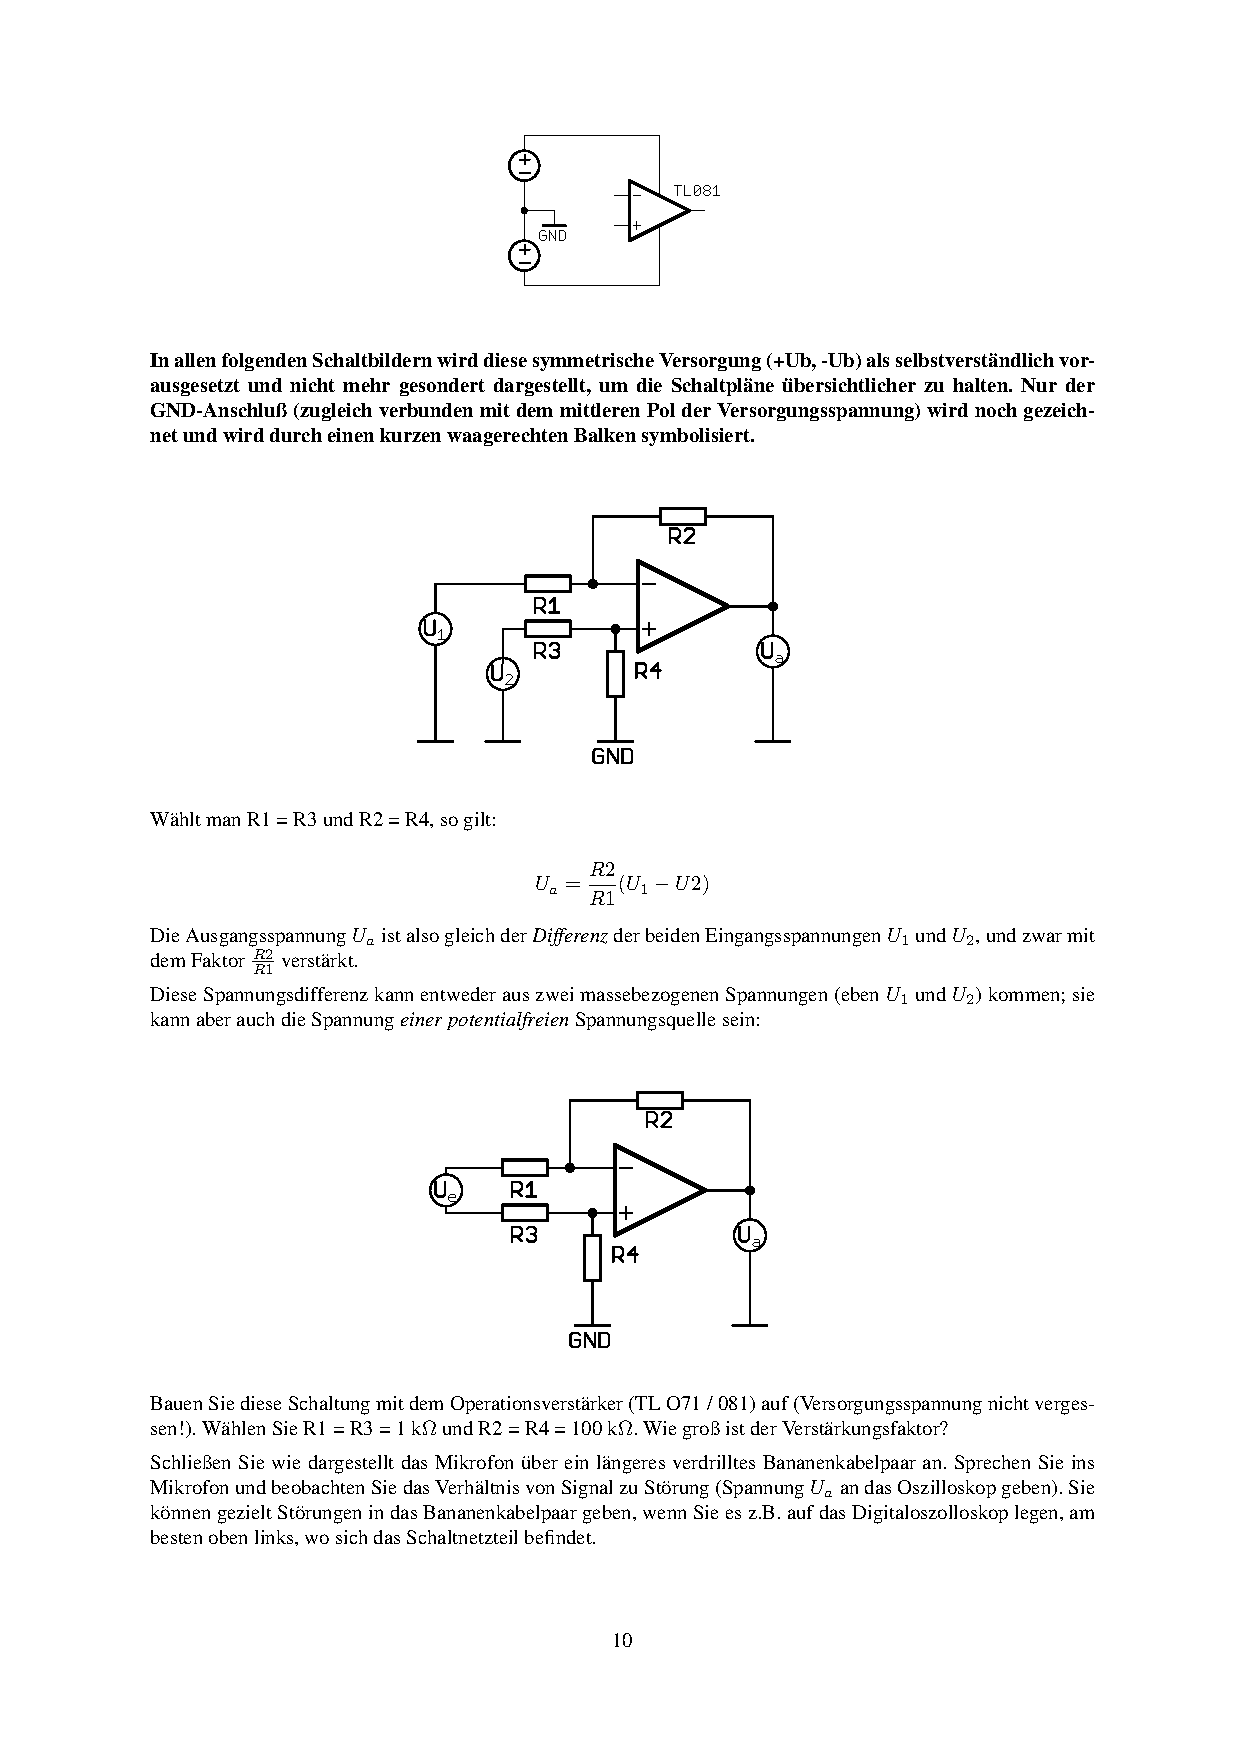
\includegraphics[trim = 10mm 240mm 10mm 15mm, clip, scale = 1]{Op-Amp.pdf}
  	\caption[Schaltskizze zum Anschlusses des Operationsverstärkers]{Schaltskizze zum Anschlusses des Operationsverstärkers\footnotemark}
  \label{fig:2.33}
\end{figure}
\footnotetext{Abbildung entnommen von http://www.atlas.uni-wuppertal.de/$\sim$kind/ep1\_14.pdf Seite 11 am 19.10.2014}

Der Operationsverstärker und das Mikrofon werden dann nach Schaltbild \ref{fig:2.4} geschaltet.
Dabei wurde für die Widerstände die Werte R$_1$=R$_3$= 1k$\Omega$ und R$_2$=R$_4$=100k$\Omega$ gewählt. Dadurch ergibt sich eine Verstärkung um den Faktor 100 \footnote{siehe Formel aus der Versuchsbeschreibung http://www.atlas.uni-wuppertal.de/$\sim$kind/ep1\_14.pdf Seite 10 am 23.10.2014}.

\begin{figure}[H] 
  \centering
    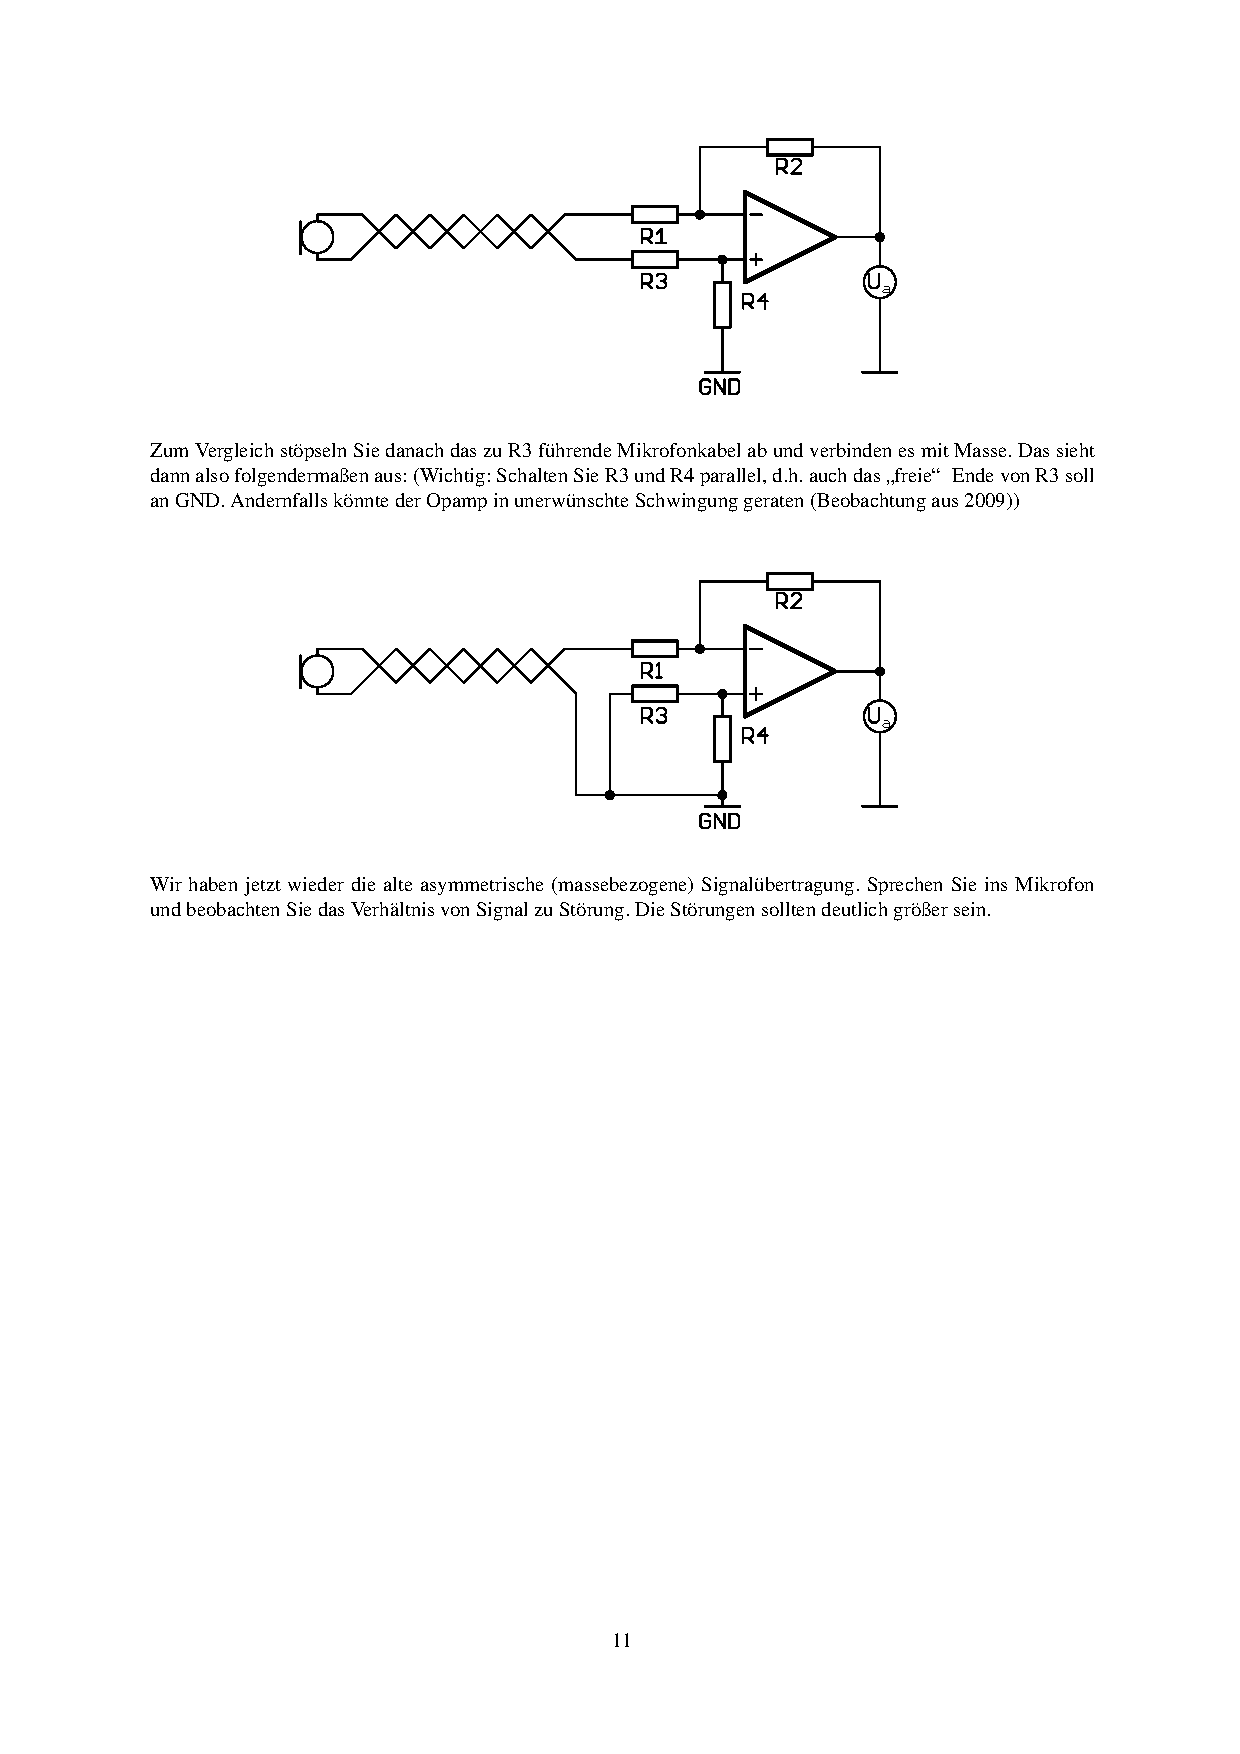
\includegraphics[trim = 10mm 230mm 10mm 20mm, clip, scale = 1]{2_3+Op-Amp.pdf}
  	\caption[Schaltskizze des Aufbaus mit Operationsverstärker und verdrillten Bananenkabeln]{Schaltskizze des Aufbaus mit Operationsverstärker und verdrillten Bananenkabeln\footnotemark}
  \label{fig:2.4}
\end{figure}
\footnotetext{Abbildung entnommen von http://www.atlas.uni-wuppertal.de/$\sim$kind/ep1\_14.pdf Seite 11 am 19.10.2014}

Zum Vergleich wird Widerstand 3 mit der Erde verbunden, Aufbau nach Abbildung \ref{fig:2.5}.

\begin{figure}[H] 
  \centering
    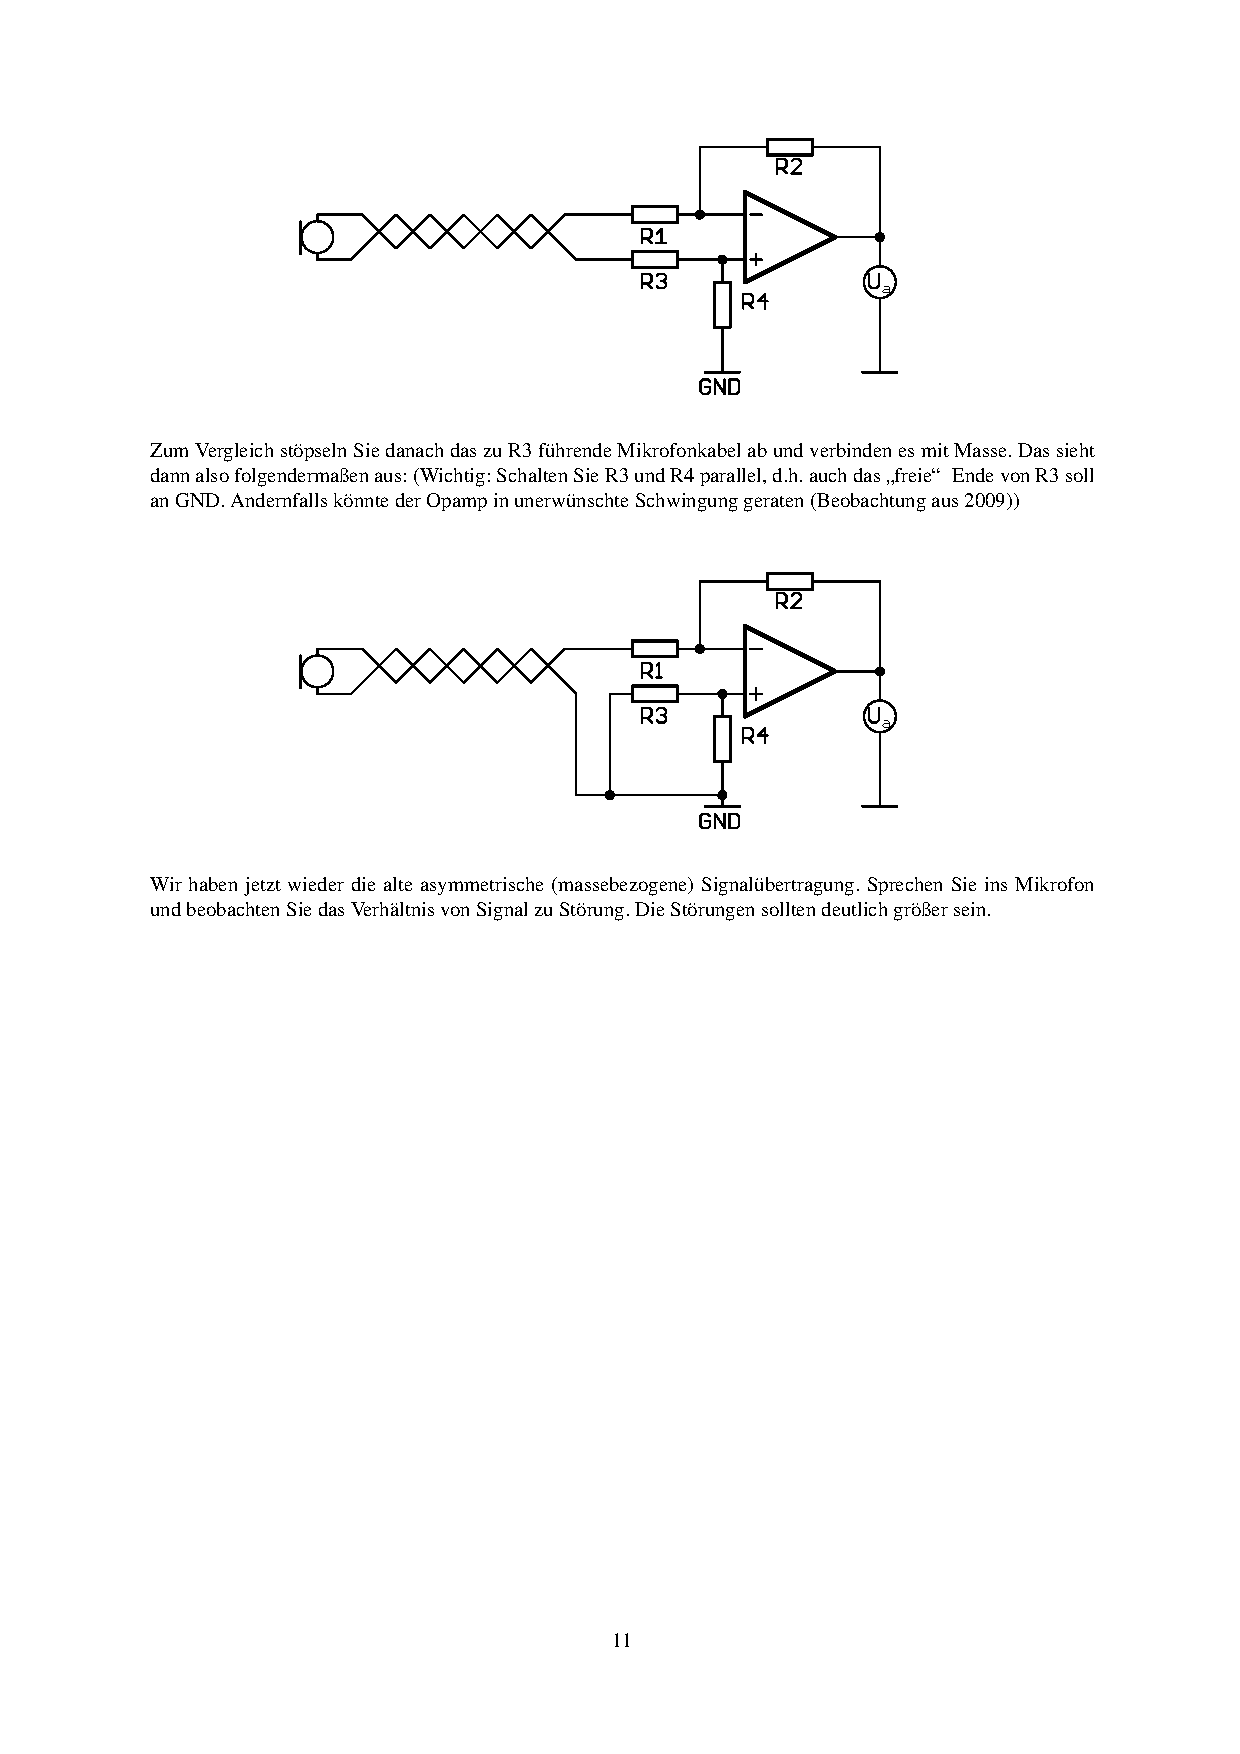
\includegraphics[trim = 10mm 160mm 10mm 90mm, clip, scale = 1]{2_3+Op-Amp.pdf}
  	\caption[Schaltskizze des Aufbaus mit Operationsverstärker und verdrillten Bananenkabeln, bei parallel geschaltetem R$_3$]{Schaltskizze des Aufbaus mit Operationsverstärker und verdrillten Bananenkabeln, bei parallel geschaltetem R$_3$\footnotemark}
  \label{fig:2.5}
\end{figure}
\footnotetext{Abbildung entnommen von http://www.atlas.uni-wuppertal.de/$\sim$kind/ep1\_14.pdf Seite 11 am 19.10.2014}


\subsection{Versuchsdurchführung}
%erklären, !was! wir machen, !warum! wir das machen und mit welchem ziel
%(wichtig) präzize erklären, wie bei dem versuch vorgegangen und was gemacht wurde
%erklären, !was! wir machen, !warum! wir das machen und mit welchem ziel
%(wichtig) präzize erklären, wie bei dem versuch vorgegangen und was gemacht wurde
An die Aufbauten in Versuchsteil 2.1 und 2.2 wurden jeweils eine Sinus- und eine Rechteckspannung angelegt und der Frequenzbereich von \unit[100]{Hz} bis \unit[10]{MHz} mit dem Oszilloskop ausgemessen. Die Verzerrungen des Signals werden anhand der Graphiken (bei gleichen Spannungsamplituden) miteinander verglichen.

Im dritten Teil werden die Bananenkabel aus dem zweiten Teil miteinander verdrillt und die Verbesserung der Signalübertragung bei kleinen Spannungsamplituden mit dem Aufbau aus dem zweiten Teil verglichen.\newline
Da die Erdung des Funktionsgenerators und des Oszilloskops nur einen kleinen Gegenstrom durch das zweite Kabel zulässt, welcher eigentlich die Störung des zweiten Kabels aufheben soll, wird anschließend das Mikrofon als Signalquelle verwendet und über einen Operationsverstärker an das Oszilloskop angeschlossen, sodass durch das zweite Kabel der entgegengesetzte Strom fließen kann. Um die Verbesserung der Signalübertragung bei diesem Microphon (dynamisches Mikrophon) gegenüber dem geerdeten Fall abzuschätzen, wird parallel zu Widerstand R3 die Erde angeschlossen, sodass das zweite Kabel wie bei dem Aufbau mit dem Funktionsgenerator direkt mit der Erde verbunden ist. Für die Signalerzeugung wurde einerseits in das Mikrophon gepfiffen und andererseits das Mikrofon auf den Funktionsgenerator gelegt um die dadurch erzeugten Störsignale aufzunehmen. Die Darstellung wurde dann jeweils auf dem Oszilloskop angehalten.

%\subsection{Verwendete Formeln}
%eine legende kann angefertigt werden, die selbstverständlichen buchstaben müssen nicht extra erklärt werden
%mit knappen erklärungen die !verwendeten! formeln, sowie die zugehörige fehlerrechnung einfügen.

%\subsection{Messergebnisse}
%die messwerte in !übersichtlichen! tabellen angegeben
%zu viele kleine tabellen in große tabellen überführen!
%zu große tabellen mit dem [scale]-befehl scalieren oder (falls zu lang) in zwei kleinere tabellen aufteilen
%(wichtig) vor !jeder! tabelle sagen, was gemessen wurde und wie die fehler gewählt wurden und ausreichend !erklären!, !warum! wir unsere fehler grade so gewählt haben
\subsection{Auswertung}
%zuerst !alle! errechneten werte entweder in ganzen sätzen aufzählen, oder in tabellen (übersichtlicher) dargestellen, sowie auf die verwendeten formeln verweisen (die referenzierung der formel kann in der überschrift stehen)
%kurz erwähnen (vor der tabelle), warum wir das ganze ausrechnen bzw. was wir dort ausrechnen
%danach histogramme und plots erstellen, wobei wenn möglich funktionen durch die plots gelegt werden (zur not können auch splines benutzt werden, was aber angegeben werden muss)
%bei fits immer die funktion und das reduzierte chiquadrat mit angegeben, wobei auf verständlichkeit beim entziffern der zehnerpotenzen geachtet werden muss z.b. f(x)=(wert+-fehler)\cdot10^{irgendeine zahl}\cdot x + (wert+-fehler)\cdot10^{irgendeine zahl}
%bei jedem fit erklären, nach welchem zusammenhang gefittet wurde und warum!
%bei plots darauf achten, dass die achsenbeschriftung (auch die tics) die richtige größe haben und die legende im plot nicht die messwerte verdeckt
%kurz die aufgabenstellung abgehandeln

In der Auswertung wird die Qualität der übertragenen Signale bei unterschiedlichen Frequenzen überprüft.

\subsubsection{2.1 Ein Bananenkabel und gemeinsame Masse}

Ersten Messung mit nur einem Bananenkabel:
Bei der Übertragung des Sinussignals war kein qualitativer Unterschied festzustellen, wie man an Abbildung \ref{fig:2_1_sin_100hz} und Abbildung \ref{fig:2_1_sin_10mhz} erkennen kann.


\begin{figure}[H]
        \centering
        \begin{subfigure}[b]{0.48\textwidth}
                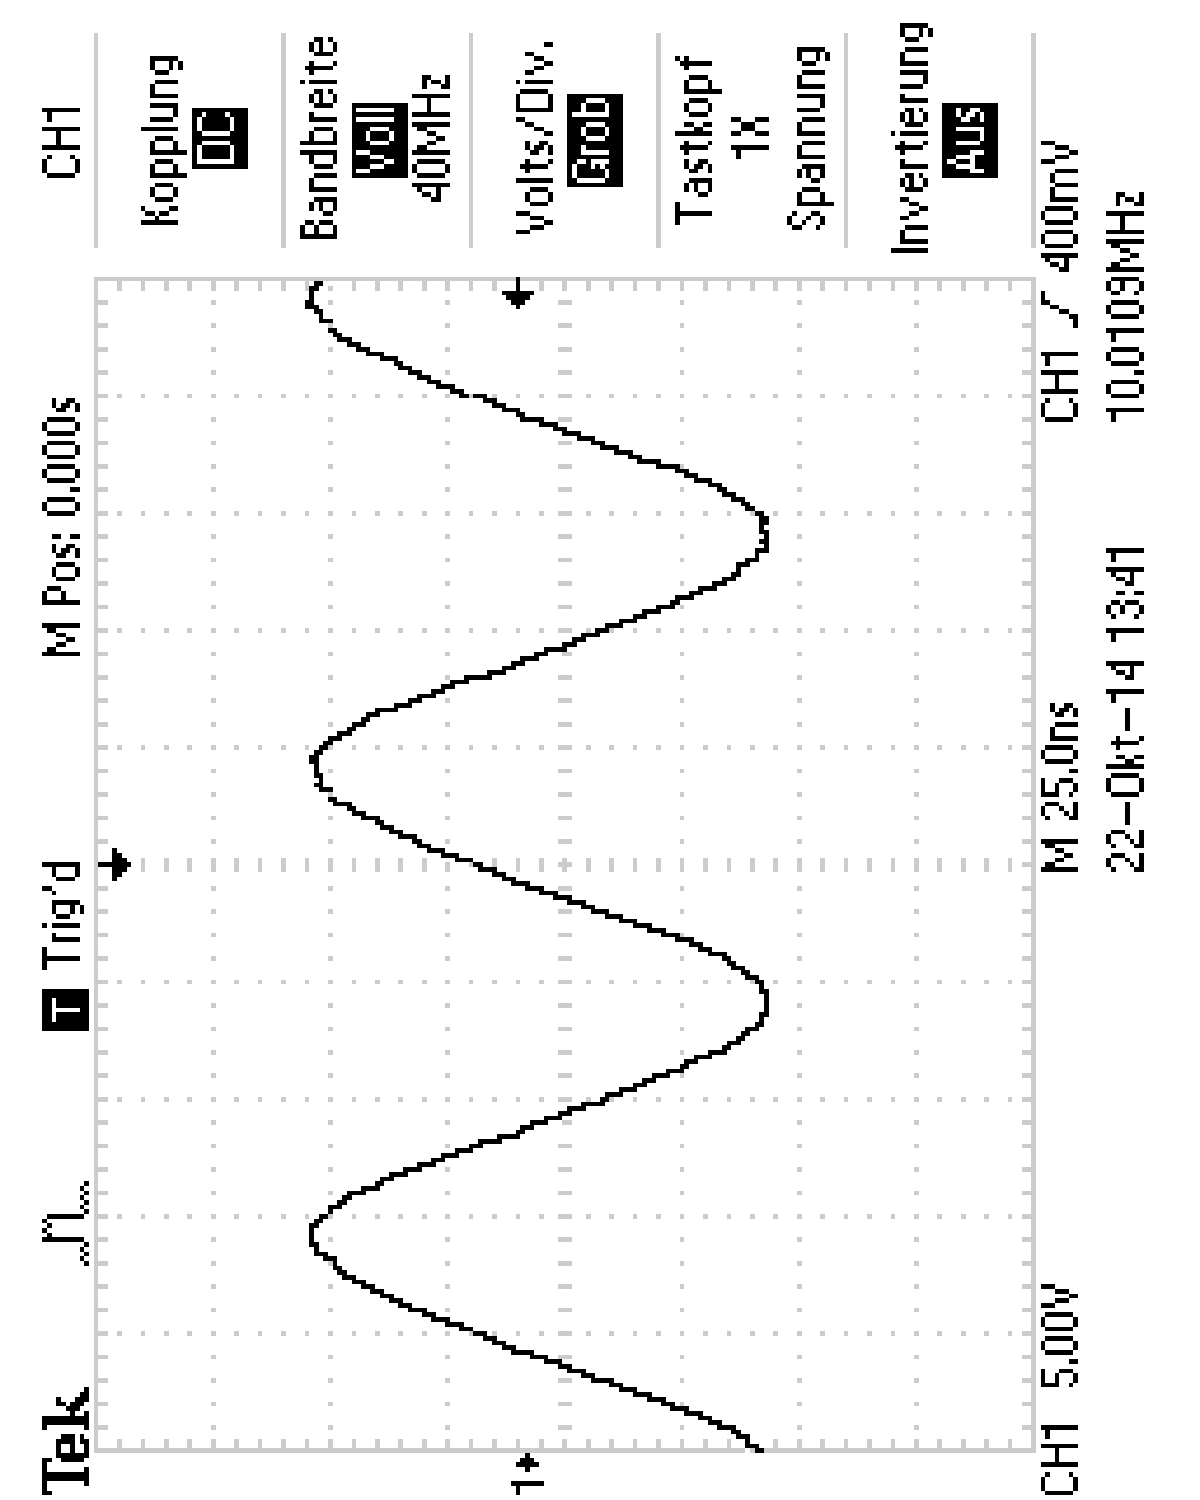
\includegraphics[width=\textwidth , scale = 0.4, angle = -90]{2_1_sin_10mhz.pdf}
                \caption[Aufnahme der Sinuswelle mit einer Frequenz von 100Hz]{Aufnahme der Sinuswelle mit einer Frequenz von 100Hz}
 				 \label{fig:2_1_sin_100hz}
        \end{subfigure}%
        ~ %add desired spacing between images, e. g. ~, \quad, \qquad, \hfill etc.
          %(or a blank line to force the subfigure onto a new line)
        \hfill
        \begin{subfigure}[b]{0.48\textwidth}
                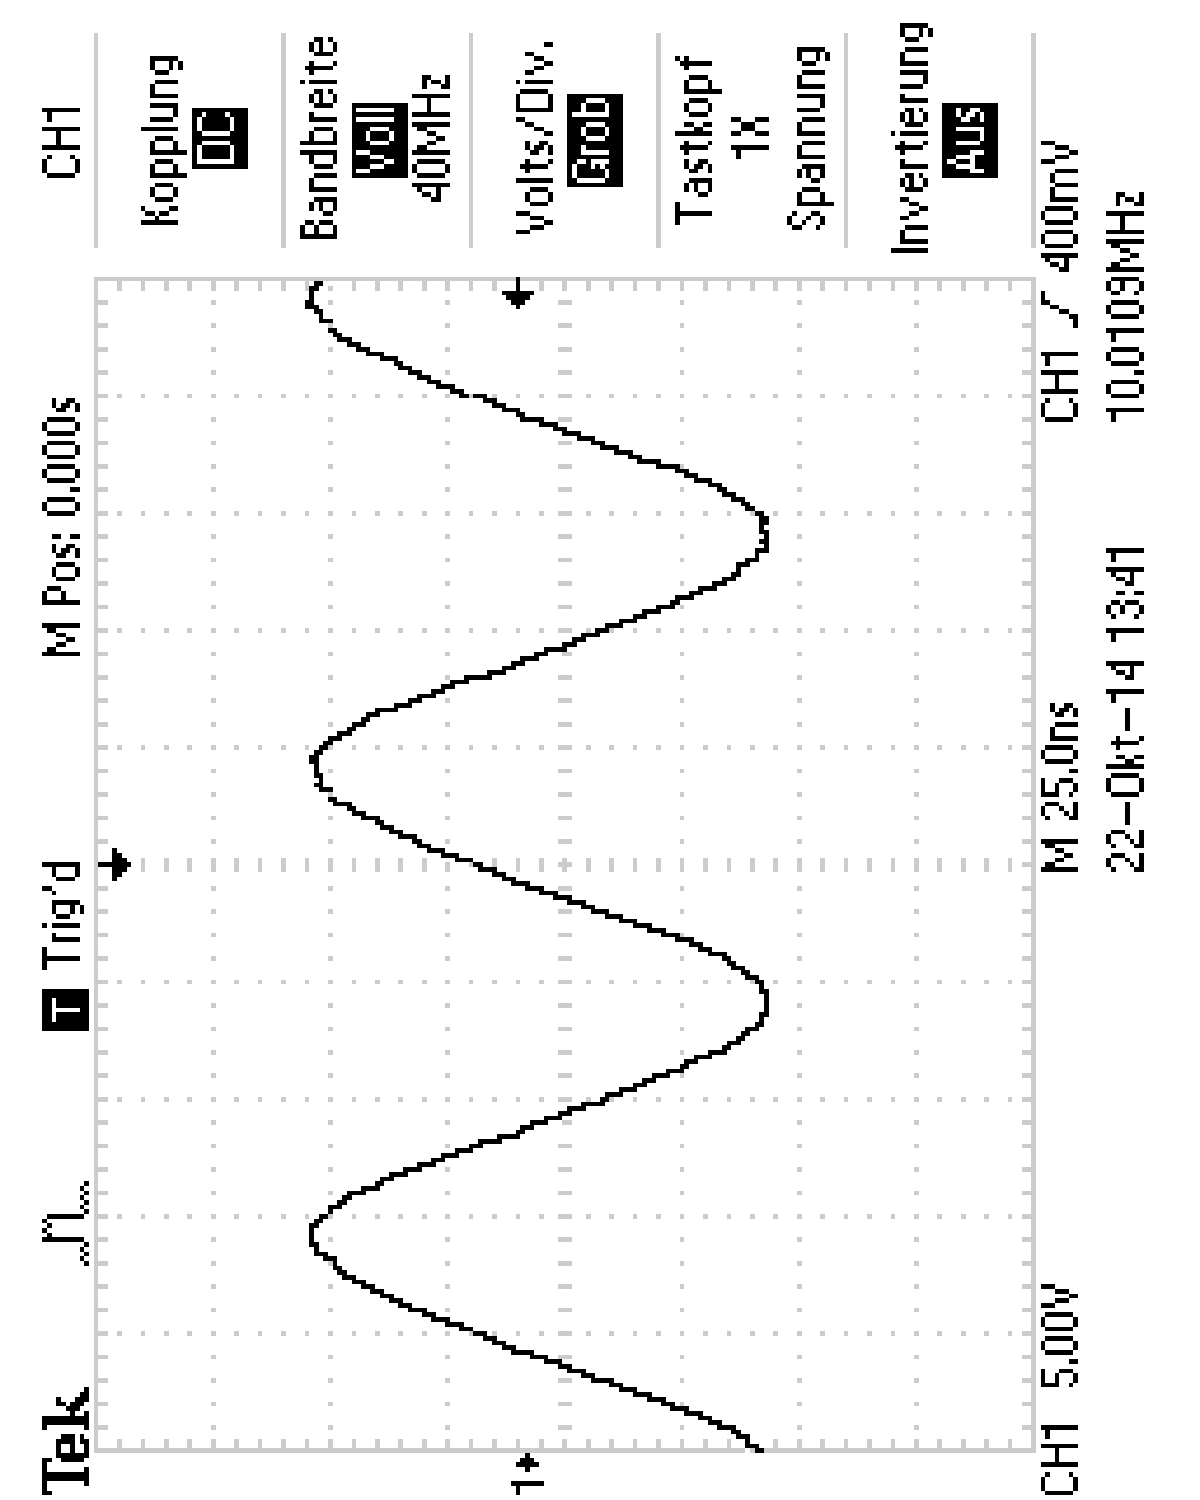
\includegraphics[width=\textwidth , scale = 0.4, angle = -90]{2_1_sin_10mhz.pdf}
                \caption[Aufnahme der Sinuswelle mit einer Frequenz von 10MHz]{Aufnahme der Sinuswelle mit einer Frequenz von 10MHz}
  				\label{fig:2_1_sin_10mhz}
        \end{subfigure}
        \caption{Kurve der übertragenen Sinussignale für 100Hz und 10MHz}
        \label{fig:2_1_sin_vergleich}
\end{figure}
\newpage 
Bei der Übertragung der Rechteckspannung war bei 100Hz noch keine Verzerrung zu sehen, siehe Abbildung \ref{fig:2_1_rech_100hz}. Die ersten Verzerrungen wurden bei einer Frequenz von 10kHz gemessen, zu sehen in Abbildung \ref{fig:2_1_rech_10khz}. Bei einer Frequenz von 10MHz ist die Rechteckspannung als solche nicht mehr zu erkennen, Abbildung \ref{fig:2_1_rech_10mhz}. Dies liegt daran, dass das Oszilloskop eine Maximale Anzeigefrequenz von 40MHz hat.

\begin{figure}[H]
        \centering
        \begin{subfigure}[b]{0.28\textwidth}
                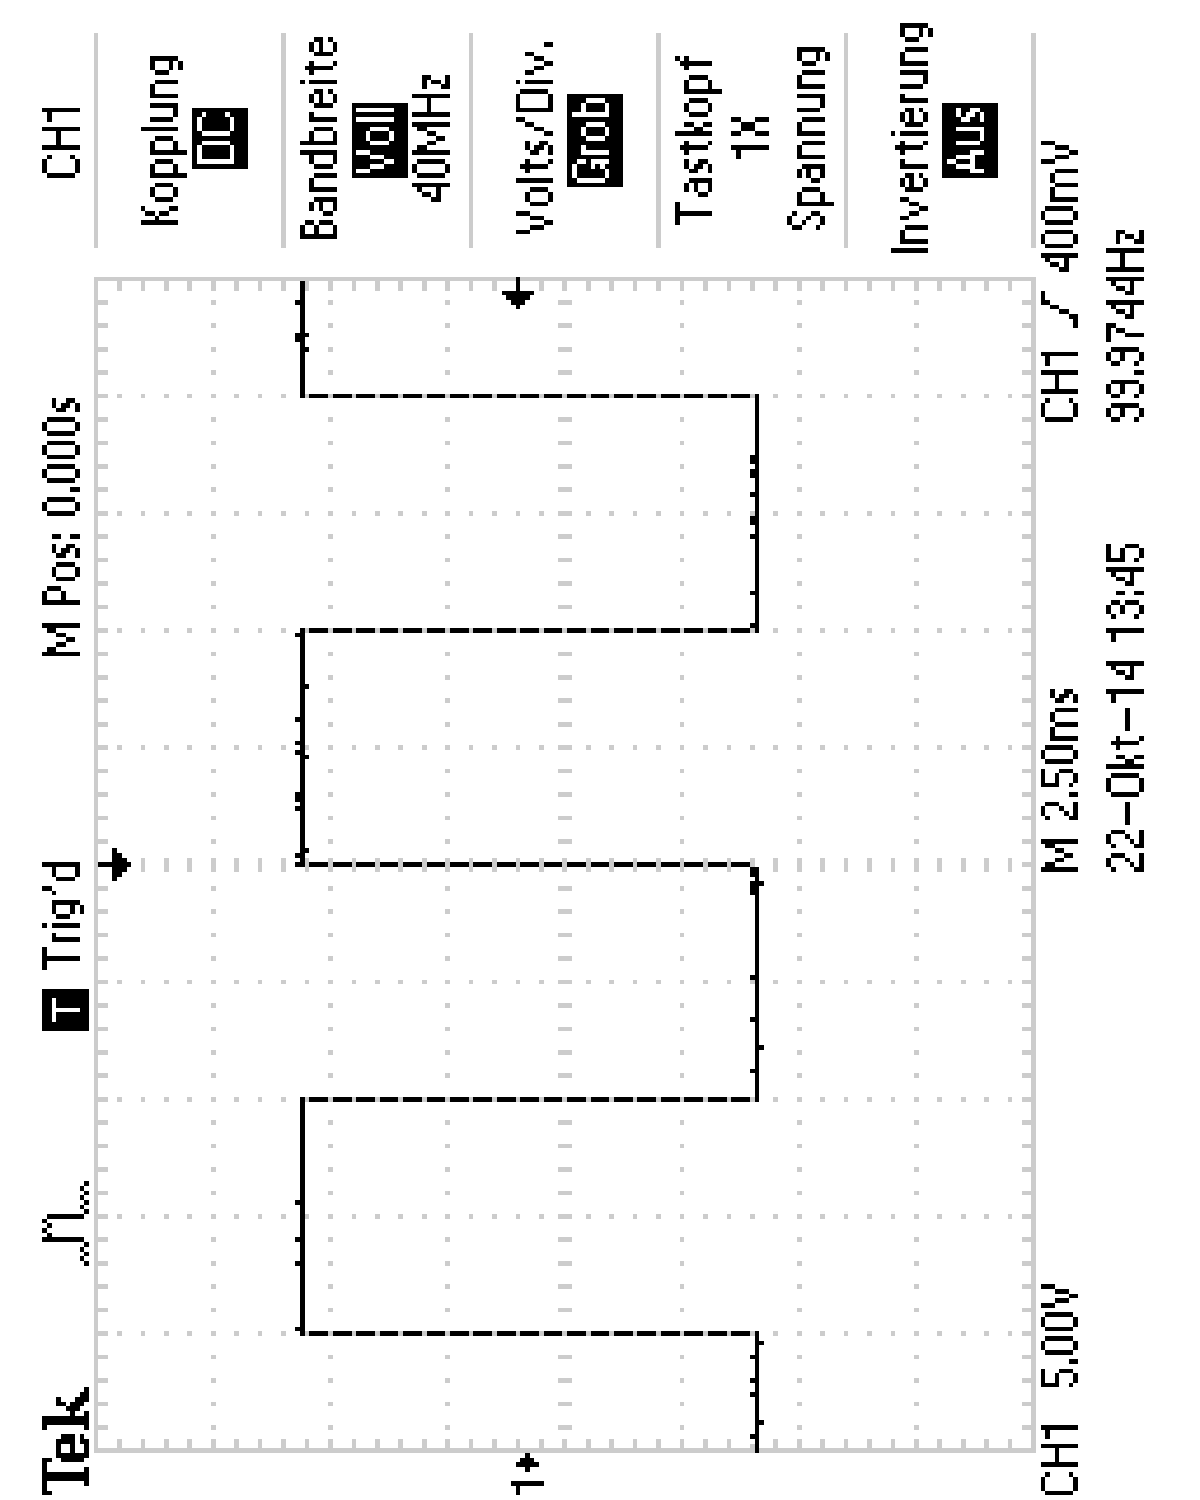
\includegraphics[width=\textwidth , scale = 0.4, angle = -90]{2_1_rech_100hz.pdf}
                \caption[Aufnahme des Rechtecksignals mit einer Frequenz von 100Hz]{Aufnahme des Rechteck Signals mit einer Frequenz von 100Hz}
                \label{fig:2_1_rech_100hz}
        \end{subfigure}%
       % ~ %add desired spacing between images, e. g. ~, \quad, \qquad, \hfill etc.
          %(or a blank line to force the subfigure onto a new line)
        \hfill
        \begin{subfigure}[b]{0.28\textwidth}
                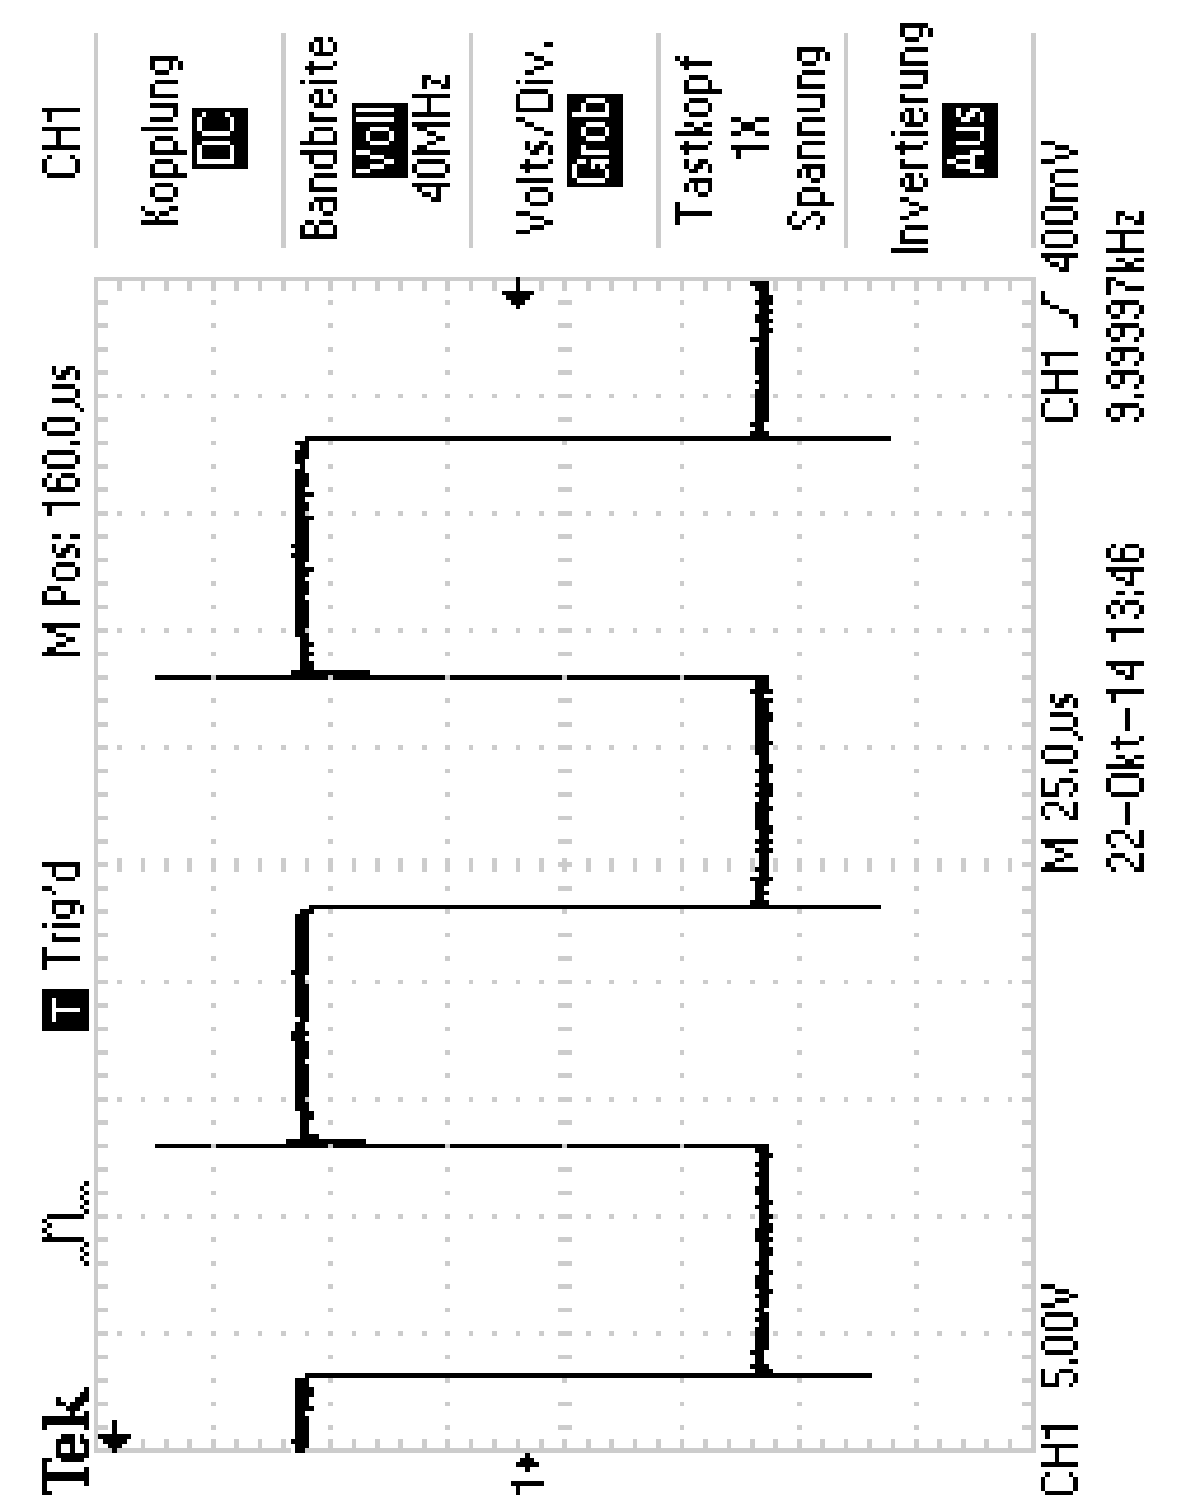
\includegraphics[width=\textwidth , scale = 0.4, angle = -90]{2_1_rech_10khz.pdf}
                \caption[Aufnahme des Rechtecksignals mit einer Frequenz von 10kHz]{Aufnahme des Rechteck Signals mit einer Frequenz von 10kHz}
                \label{fig:2_1_rech_10khz}
        \end{subfigure}
       % ~ %add desired spacing between images, e. g. ~, \quad, \qquad, \hfill etc.
          %(or a blank line to force the subfigure onto a new line)
        \hfill
        \begin{subfigure}[b]{0.28\textwidth}
                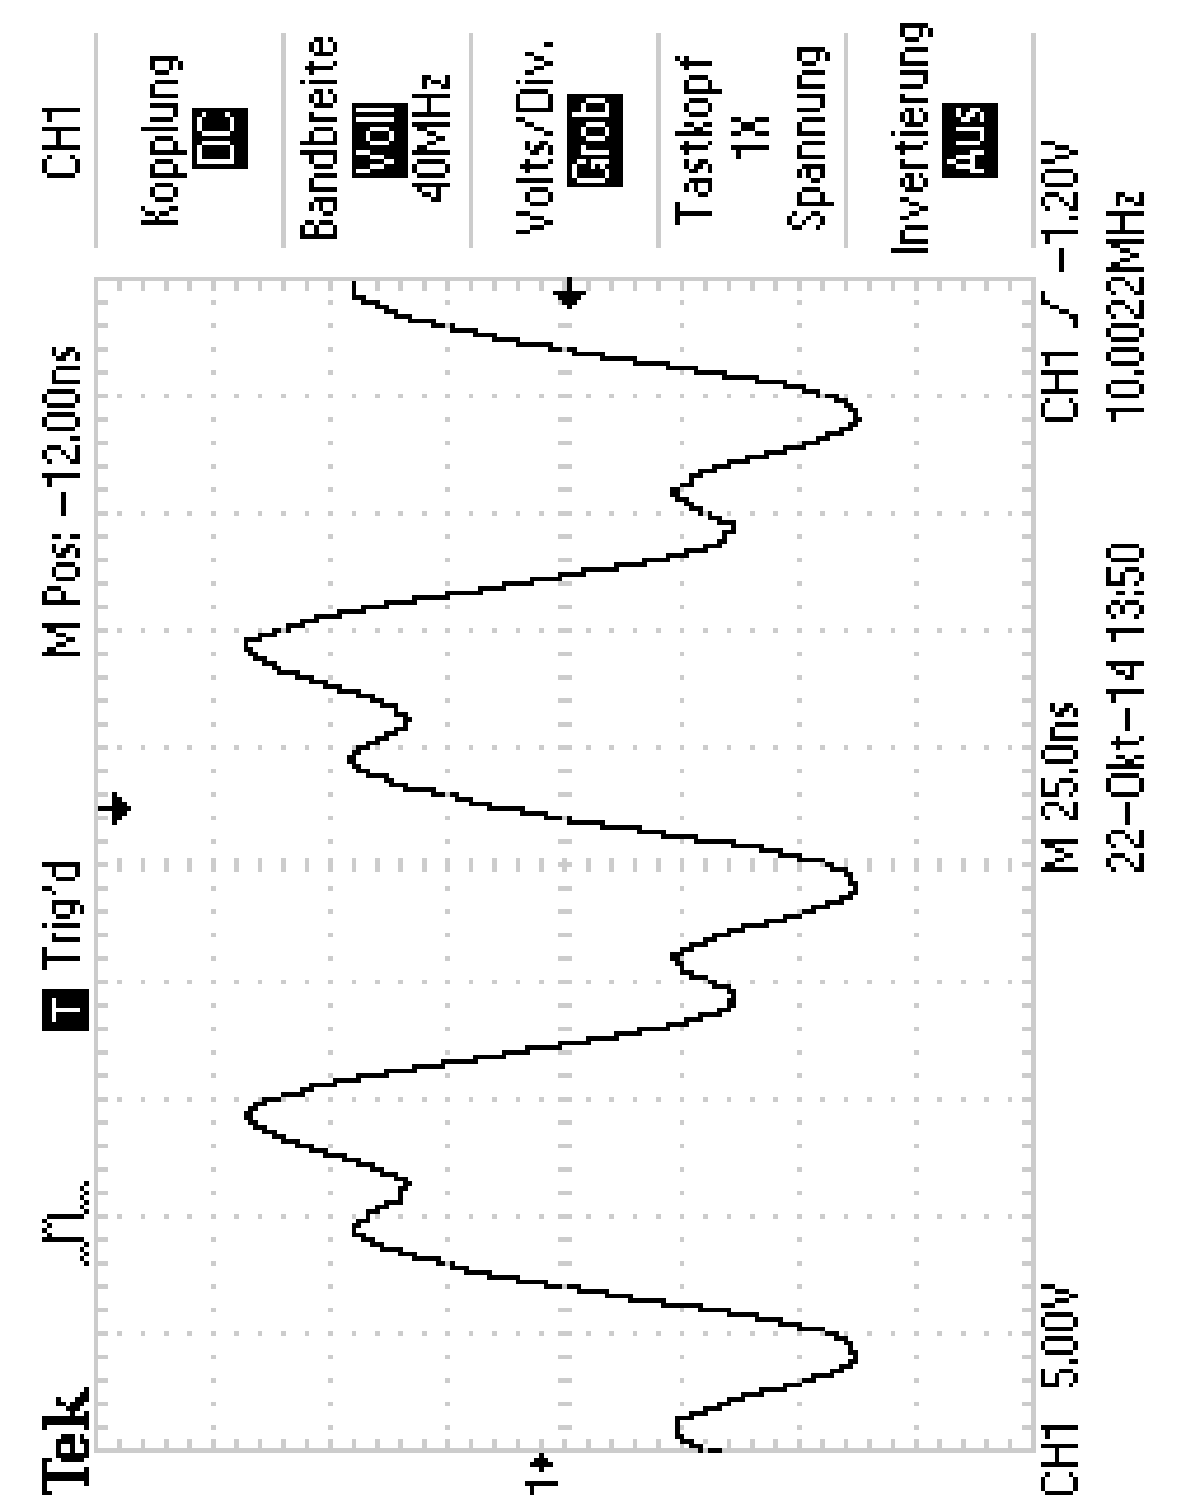
\includegraphics[width=\textwidth , scale = 0.4, angle = -90]{2_1_rech_10mhz.pdf}
                \caption[Aufnahme des Rechtecksignals mit einer Frequenz von 10MHz]{Aufnahme des Rechteck Signals mit einer Frequenz von 10MHz}
  				\label{fig:2_1_rech_10mhz}
        \end{subfigure}
        \caption{Kurve der übertragenen Rechtecksignale für 100Hz,10kHz und 10MHz}
        \label{fig:2_1_rech_vergleich}
\end{figure}



\subsubsection{2.2 Zwei Bananenkabel}


Bei der Messung mit zwei Bananenkabeln war die Qualität des Sinussignals bei unterschiedlichen Frequenzen unverändert, was in Abbildung \ref{fig:2_2_sin_vergleich} zu sehen ist.


\begin{figure}[H]
        \centering
        \begin{subfigure}[b]{0.48\textwidth}
                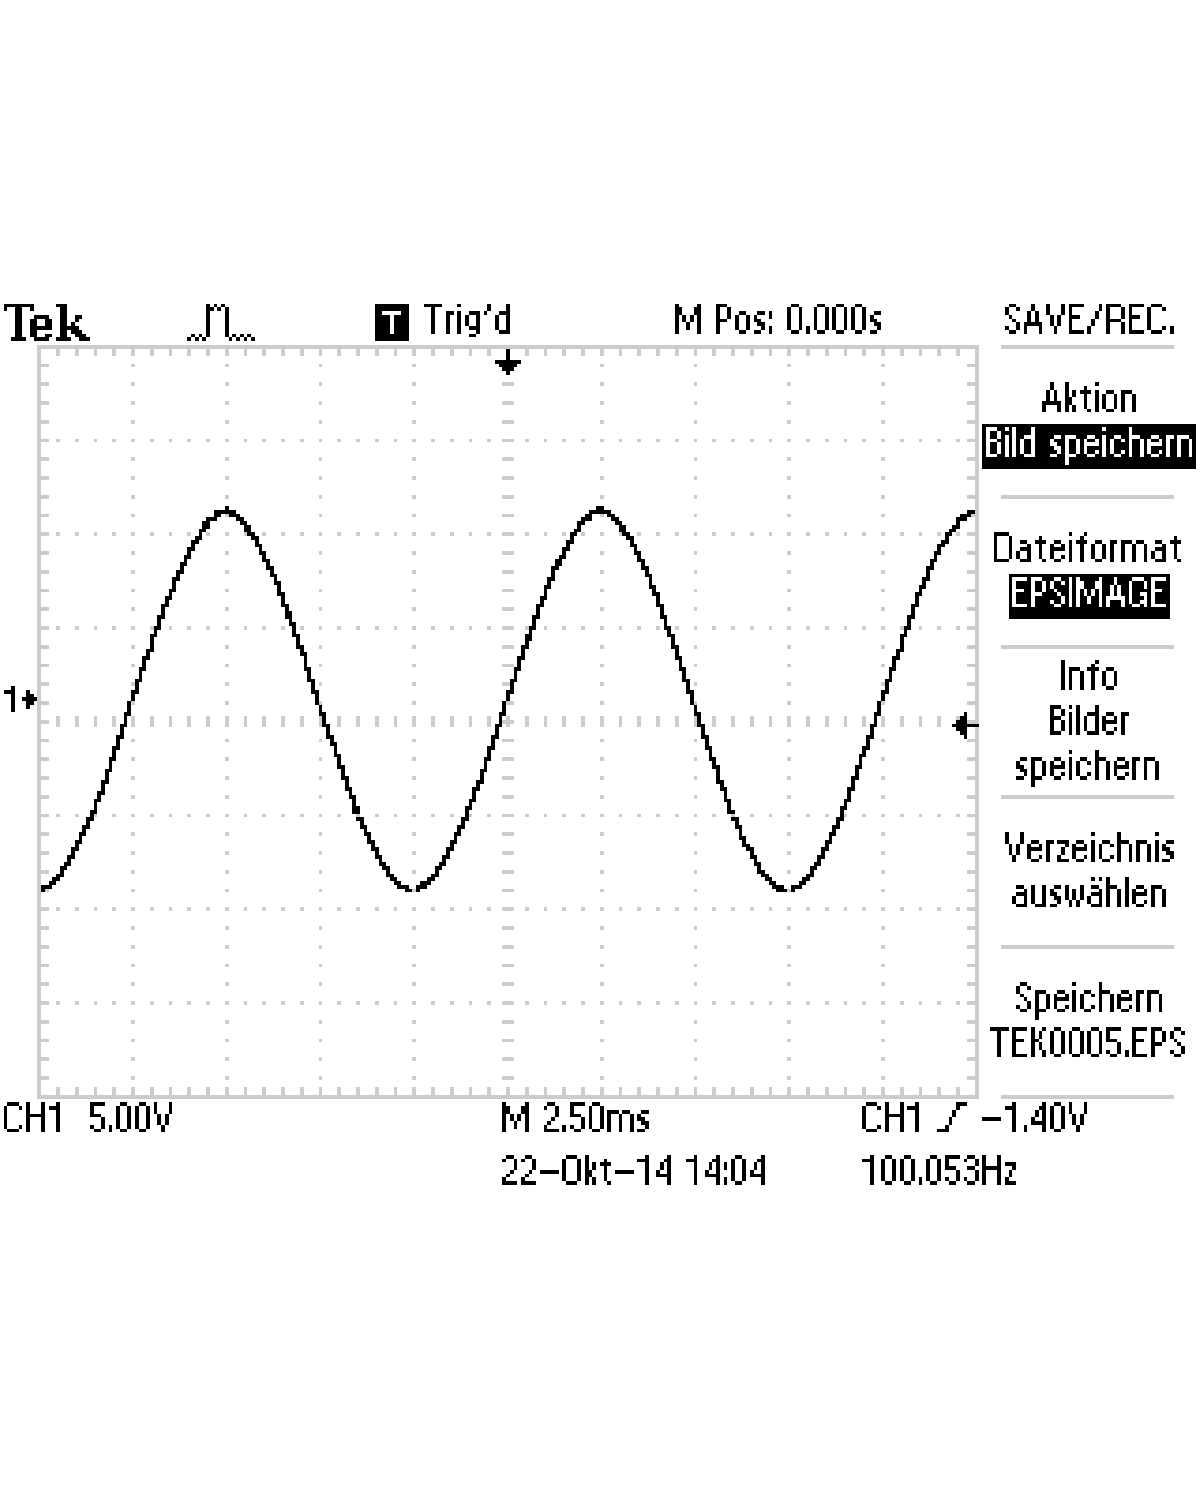
\includegraphics[width=\textwidth , scale = 0.4]{2_2_sin_100hz.pdf}
                \caption[Aufnahme der Sinuswelle mit einer Frequenz von 100Hz]{Aufnahme der Sinuswelle mit einer Frequenz von 100Hz}
 				 \label{fig:2_2_sin_100hz}
        \end{subfigure}%
        %~ %add desired spacing between images, e. g. ~, \quad, \qquad, \hfill etc.
          %(or a blank line to force the subfigure onto a new line)
        \hfill
        \begin{subfigure}[b]{0.48\textwidth}
                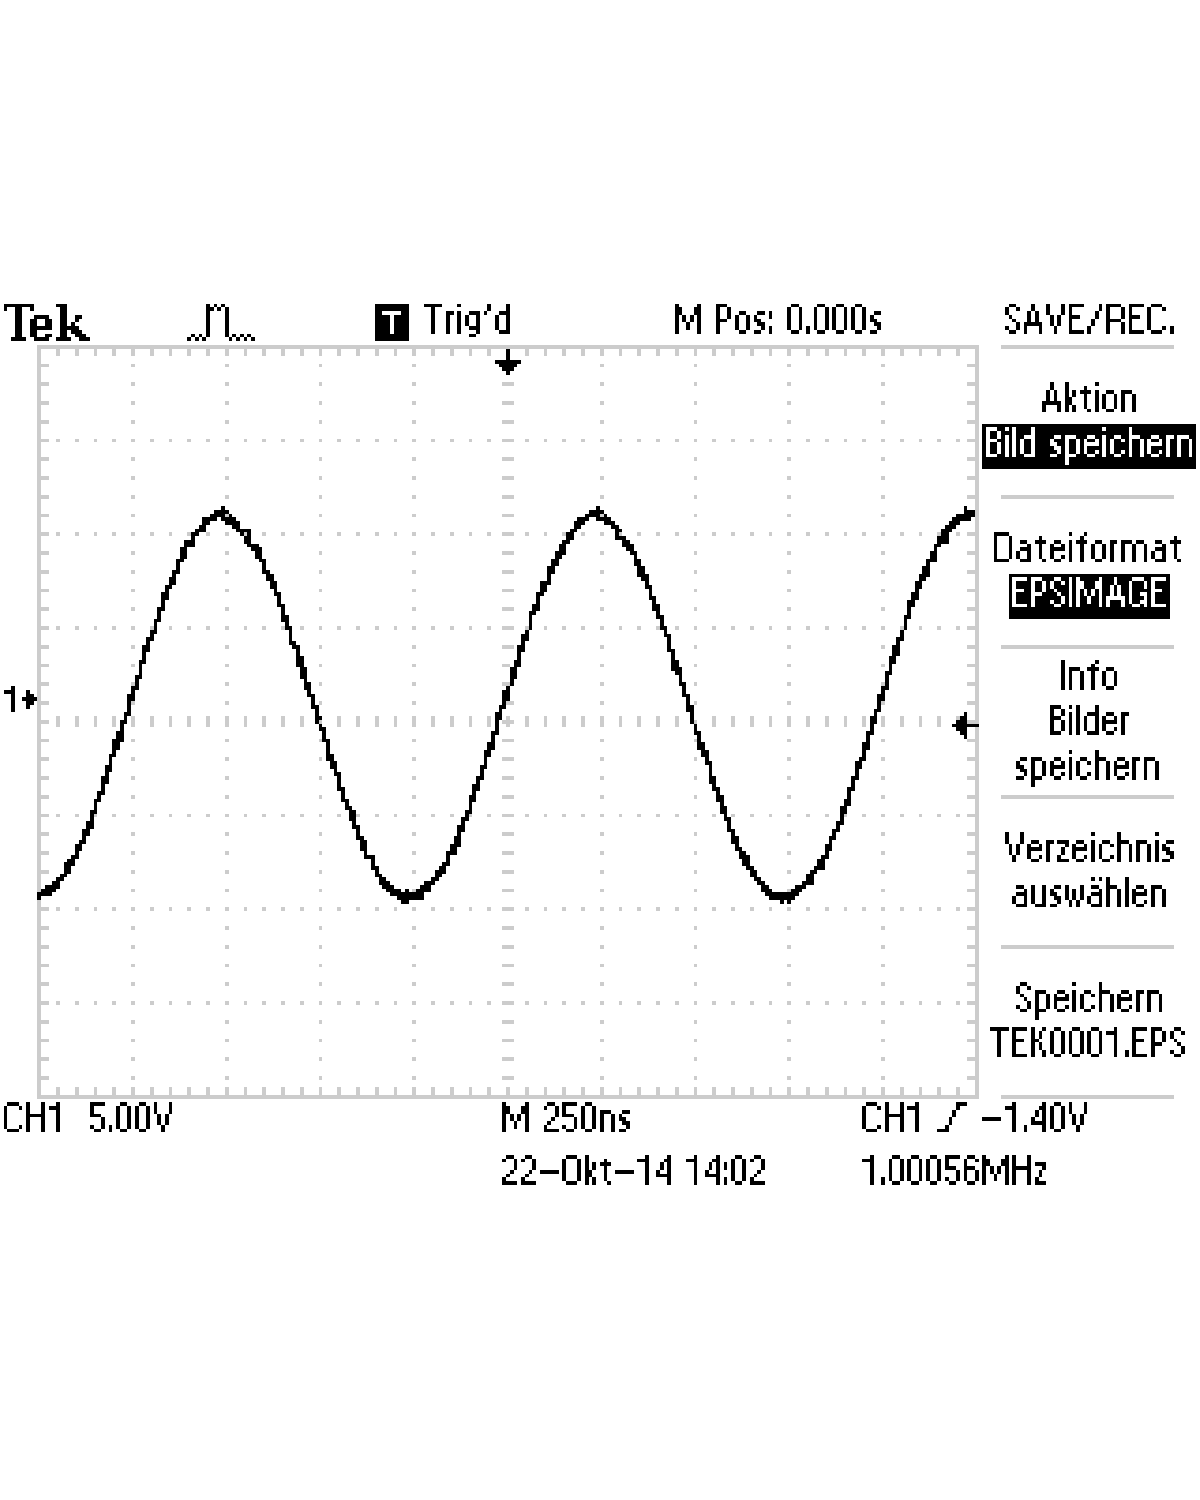
\includegraphics[width=\textwidth , scale = 0.4]{2_2_sin_1mhz.pdf}
                \caption[Aufnahme der Sinuswelle mit einer Frequenz von 1MHz]{Aufnahme der Sinuswelle mit einer Frequenz von 1MHz}
  				\label{fig:2_2_sin_1mhz}
        \end{subfigure}
        \caption{Kurve der übertragenen Sinussignale für 100Hz und 1MHz}
        \label{fig:2_2_sin_vergleich}
\end{figure}

Bei niedriger Frequenz ist das Signal sehr gut zu erkennen, Abbildung \ref{fig:2_2_rech_100hz}.
Die ersten Verzerrungen waren auch wieder bei einer Frequenz von 10kHz zu erkennen, diese fällt jedoch geringer als beim Aufbau zuvor aus, wie in Abbildung \ref{fig:2_2_rech_10khz} zu erkennen ist, was wie zuvor am Anzeigebereich des Oszilloskops liegt.
Bei einer Frequenz von 10MHz ist das vorherige Rechtecksignal als solches nicht mehr zu erkennen. Jedoch ist das Signal deutlich besser erhalten, als bei der einkanaligen Verbindung, wie in Abbildung \ref{fig:2_2_rech_10mhz} zu erkennen ist.


\begin{figure}[H]
        \centering
        \begin{subfigure}[b]{0.28\textwidth}
                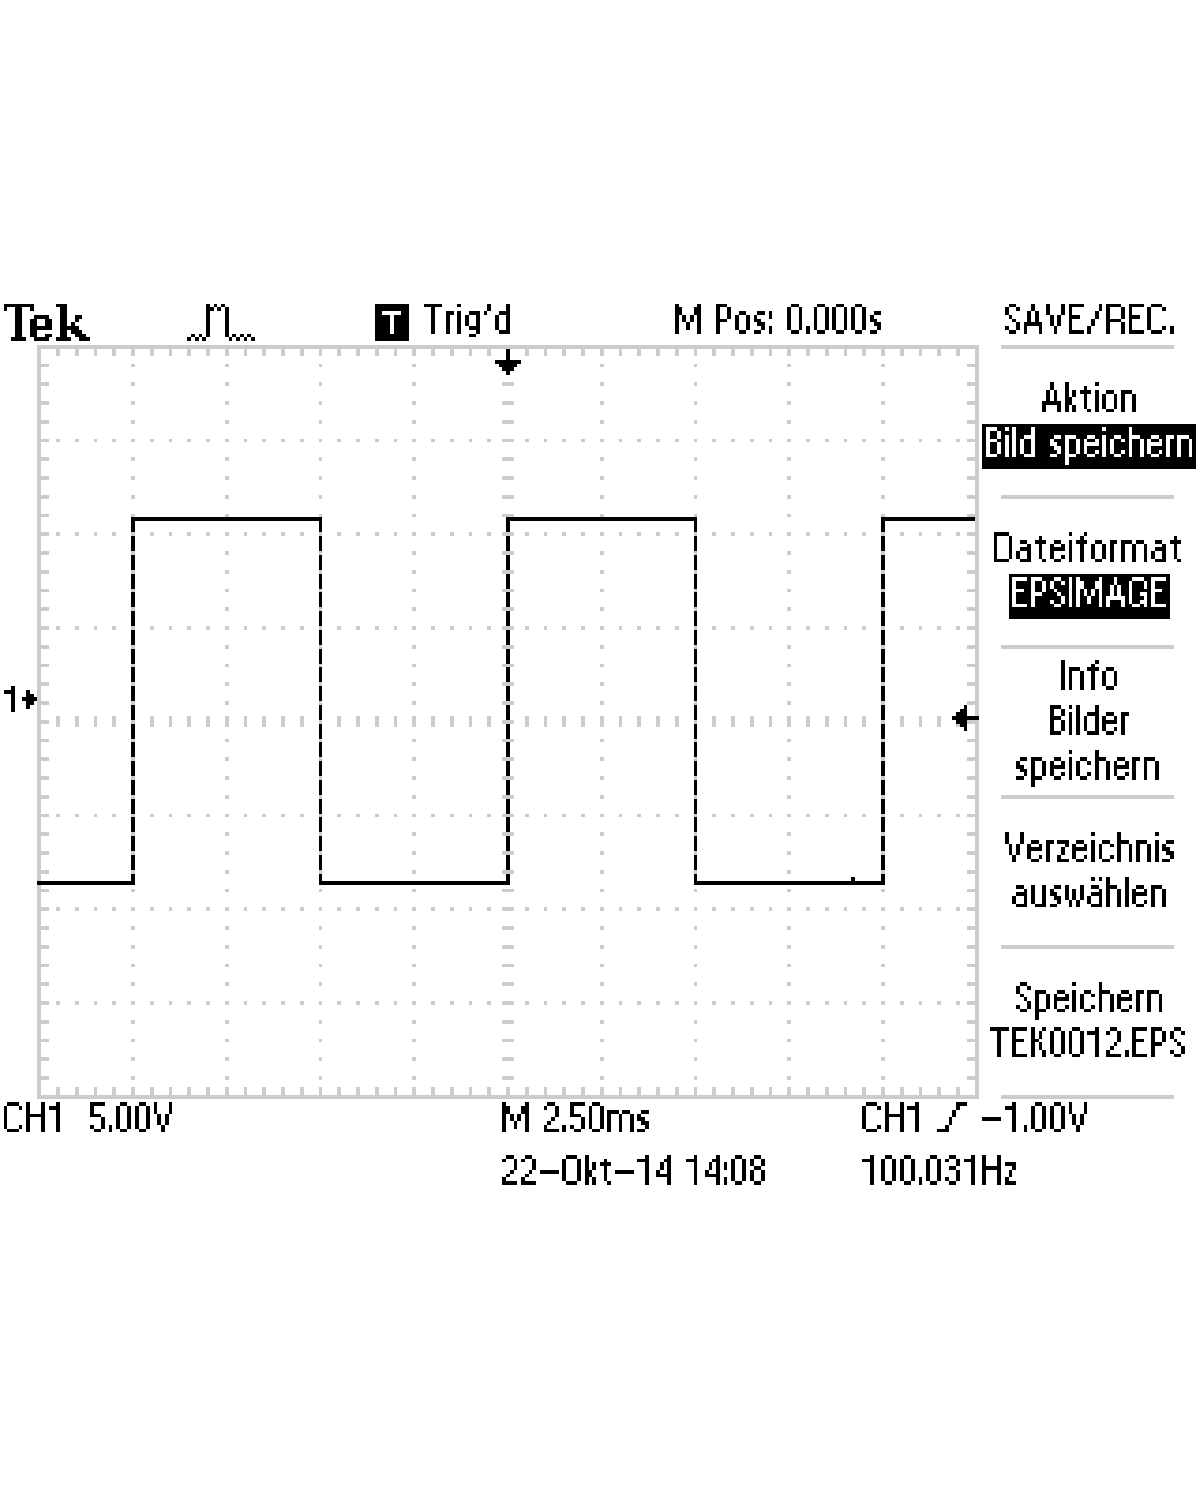
\includegraphics[width=\textwidth , scale = 0.4]{2_2_rech_100hz.pdf}
                \caption[Aufnahme des Rechtecksignals mit einer Frequenz von 100Hz]{Aufnahme des Rechteck Signals mit einer Frequenz von 100Hz}
                \label{fig:2_2_rech_100hz}
        \end{subfigure}%
        %~ %add desired spacing between images, e. g. ~, \quad, \qquad, \hfill etc.
          %(or a blank line to force the subfigure onto a new line)
        \hfill
        \begin{subfigure}[b]{0.28\textwidth}
                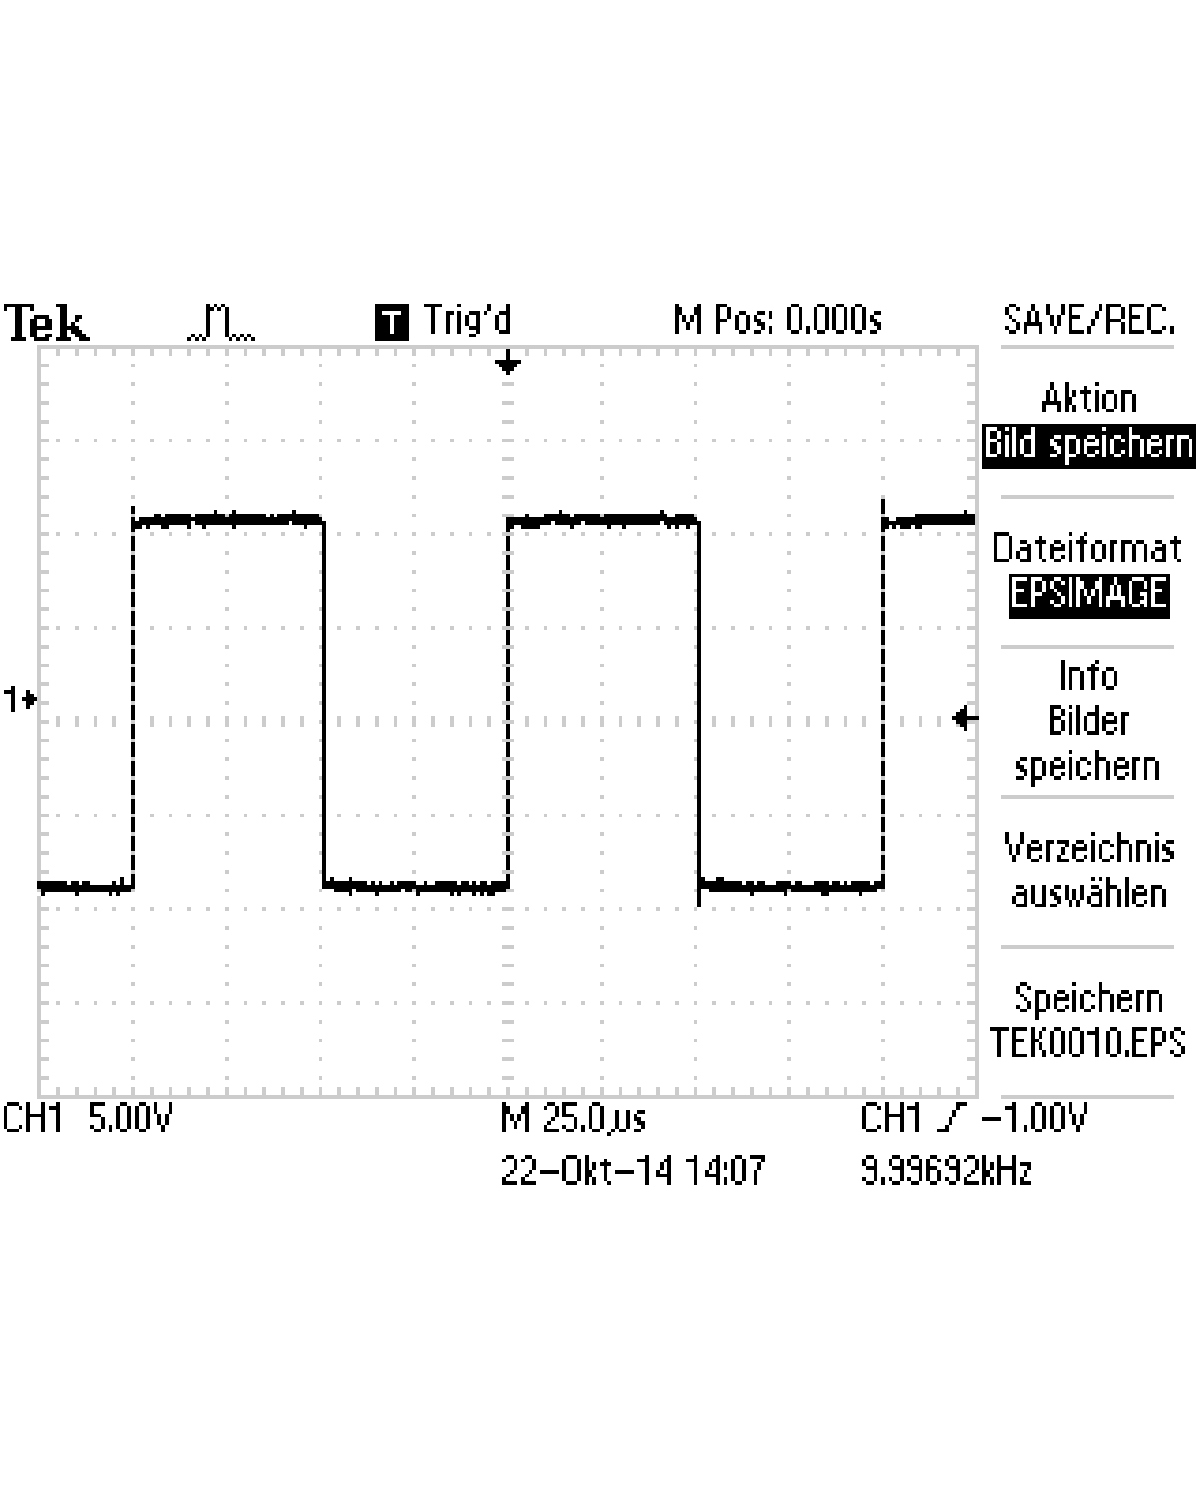
\includegraphics[width=\textwidth , scale = 0.4]{2_2_rech_10khz.pdf}
                \caption[Aufnahme des Rechtecksignals mit einer Frequenz von 10kHz]{Aufnahme des Rechteck Signals mit einer Frequenz von 10kHz}
                \label{fig:2_2_rech_10khz}
        \end{subfigure}
        %~ %add desired spacing between images, e. g. ~, \quad, \qquad, \hfill etc.
          %(or a blank line to force the subfigure onto a new line)
        \hfill
        \begin{subfigure}[b]{0.28\textwidth}
                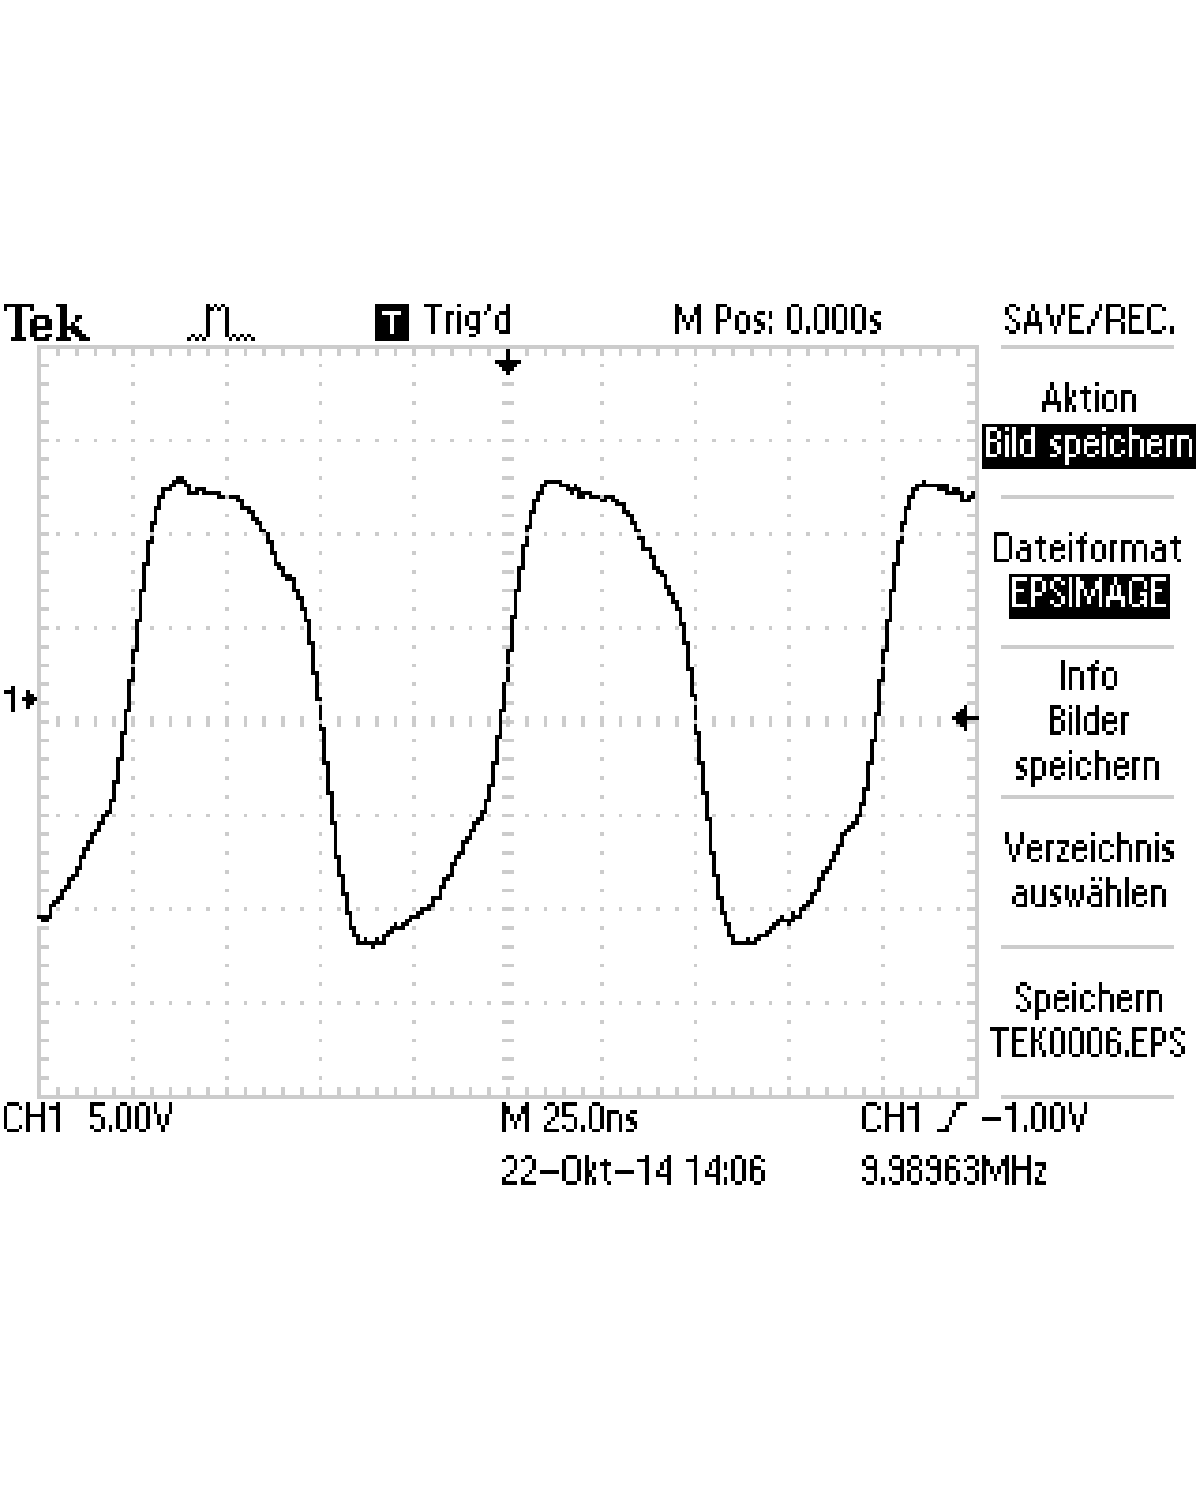
\includegraphics[width=\textwidth , scale = 1]{2_2_rech_10mhz.pdf}
                \caption[Aufnahme des Rechtecksignals mit einer Frequenz von 10MHz]{Aufnahme des Rechteck Signals mit einer Frequenz von 10MHz}
  				\label{fig:2_2_rech_10mhz}
        \end{subfigure}
        \caption{Kurve der übertragenen Rechtecksignale für 100Hz,10kHz und 10MHz}
        \label{fig:2_2_rech_vergleich}
\end{figure}
\newpage
\subsubsection{2.3 Zwei verdrillte Bananenkabel}

Betrachtet man die Signalübertragung einer Rechteckspannung mit einem twisted-pair Kabel, Abbildung \ref{fig:2_3_vgl_2} und zwei nicht verdrillten Bananenkabeln, Abbildung \ref{fig:2_3_vgl_1} so lässt sich kaum eine Verbesserung feststellen, da die Signalquelle nicht potentialfrei ist.

\begin{figure}[H]
        \centering
        \begin{subfigure}[tb]{0.48\textwidth}
                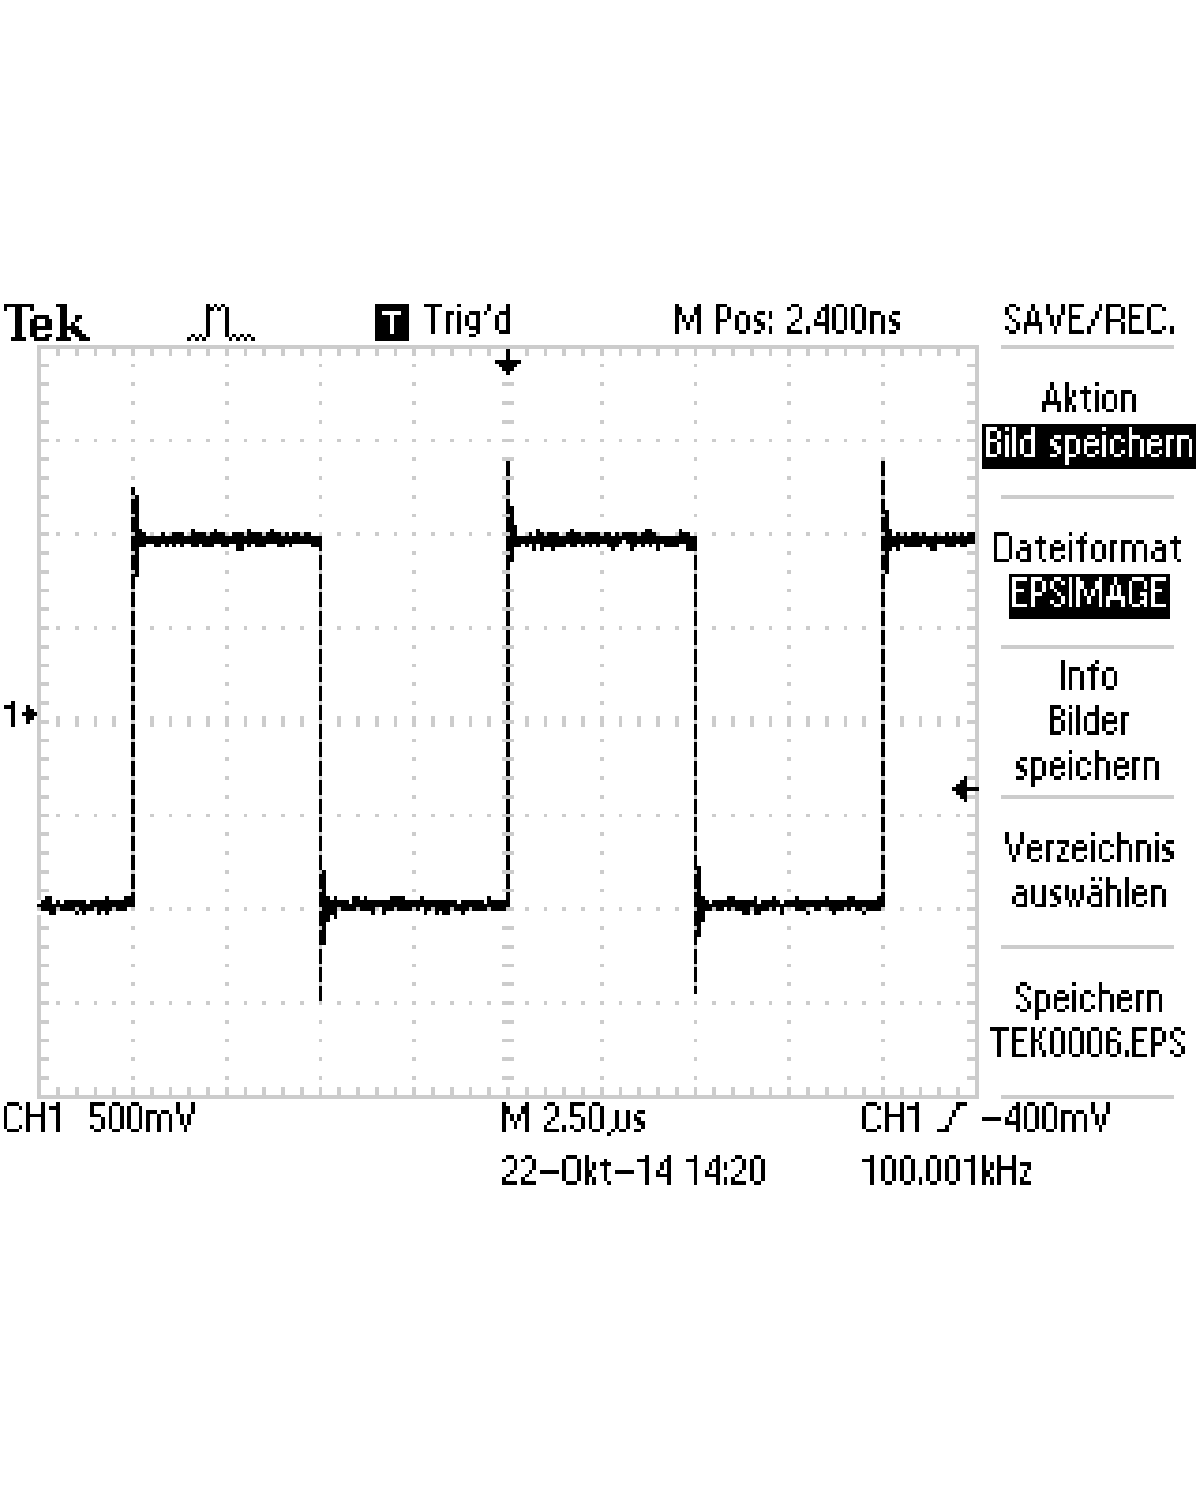
\includegraphics[width=\textwidth , scale = 0.4]{2_3_vgl_2.pdf}
				\caption[Aufnahme des Rechtecksignals, übertragen mit zwei Bananenkabel und einer Frequenz von 100kHz]{Aufnahme des Rechtecksignals, übertragen mit zwei Bananenkabel und einer Frequenz von 100kHz}
 				\label{fig:2_3_vgl_2}
        \end{subfigure}%
       % ~ %add desired spacing between images, e. g. ~, \quad, \qquad, \hfill etc.
          %(or a blank line to force the subfigure onto a new line)
        \hfill
        \begin{subfigure}[tb]{0.48\textwidth}
                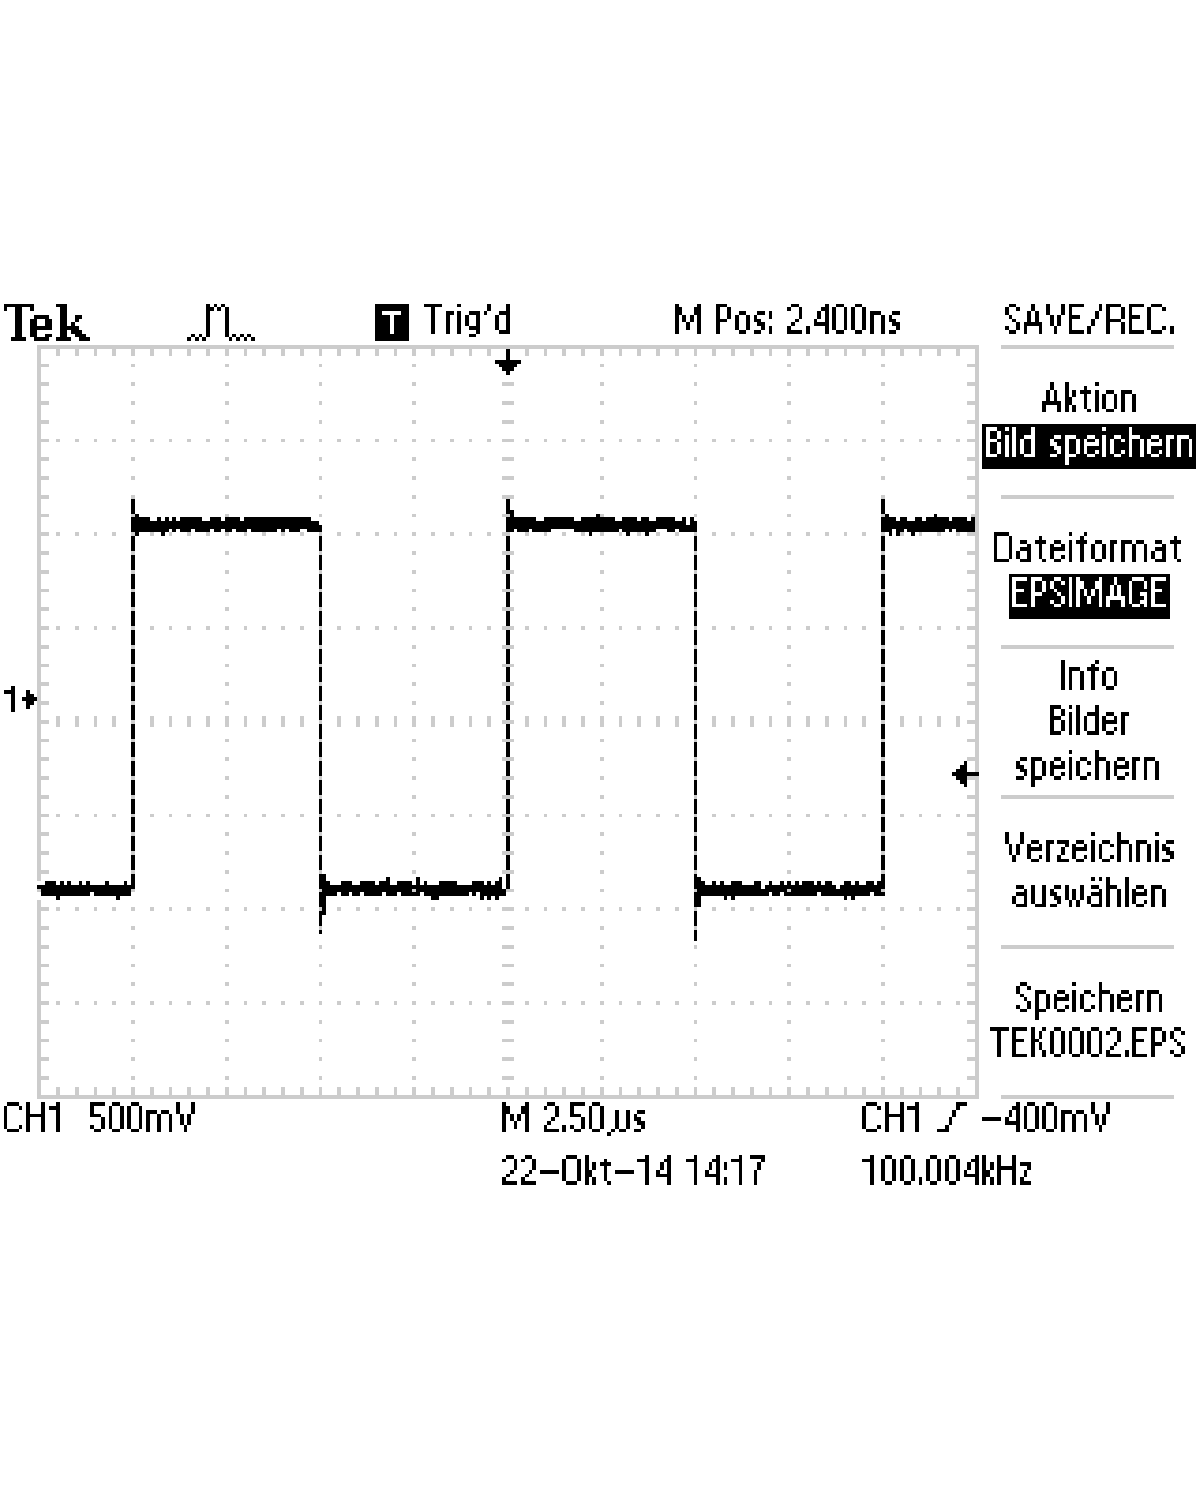
\includegraphics[trim = 0mm 0mm
                0mm 5mm ,width=\textwidth , scale = 0.4]{2_3_vgl_1.pdf}
                \caption[Aufnahme des Rechtecksignals, übertragen mit zwei verdrillten Bananenkabeln und einer Frequenz von 100kHz]{Aufnahme des Rechtecksignals, übertragen mit zwei verdrillten Bananenkabeln und einer Frequenz von 100kHz}
 				\label{fig:2_3_vgl_1}
        \end{subfigure}
        \caption{Kurve der übertragenen Sinussignale für 100Hz und 1MHz}
        \label{fig:2_3_rech_vergleich_ohne_mikro}
\end{figure}
\newpage

Bei der Messung mit dem Mikrofon ergab sich beim Aufbau nach Abbildung \ref{fig:2.4} die in Abbildung \ref{fig:2_3_r3np_sig} dargestellte Kurve. Für den Aufbau nach Abbildung \ref{fig:2.5} ergab sich die Kurve in Abbildung \ref{fig:2_3_r3p_sig}. Dabei ist zu erkennen, dass die Verzerrung des Signals an den Extrema in Abbildung \ref{fig:2_3_r3p_sig} größer ist als in Abbildung \ref{fig:2_3_r3np_sig}. Dies liegt daran, dass R$_3$ an die Masse angeschlossen ist.
Falls erwähnt wird, dass R$_3$ parallel zu R$_4$ liegt, ist impliziert, dass R$_3$ auch an die Masse angeschlossen ist.


\begin{figure}[H]
        \centering
        \begin{subfigure}[tb]{0.48\textwidth}
                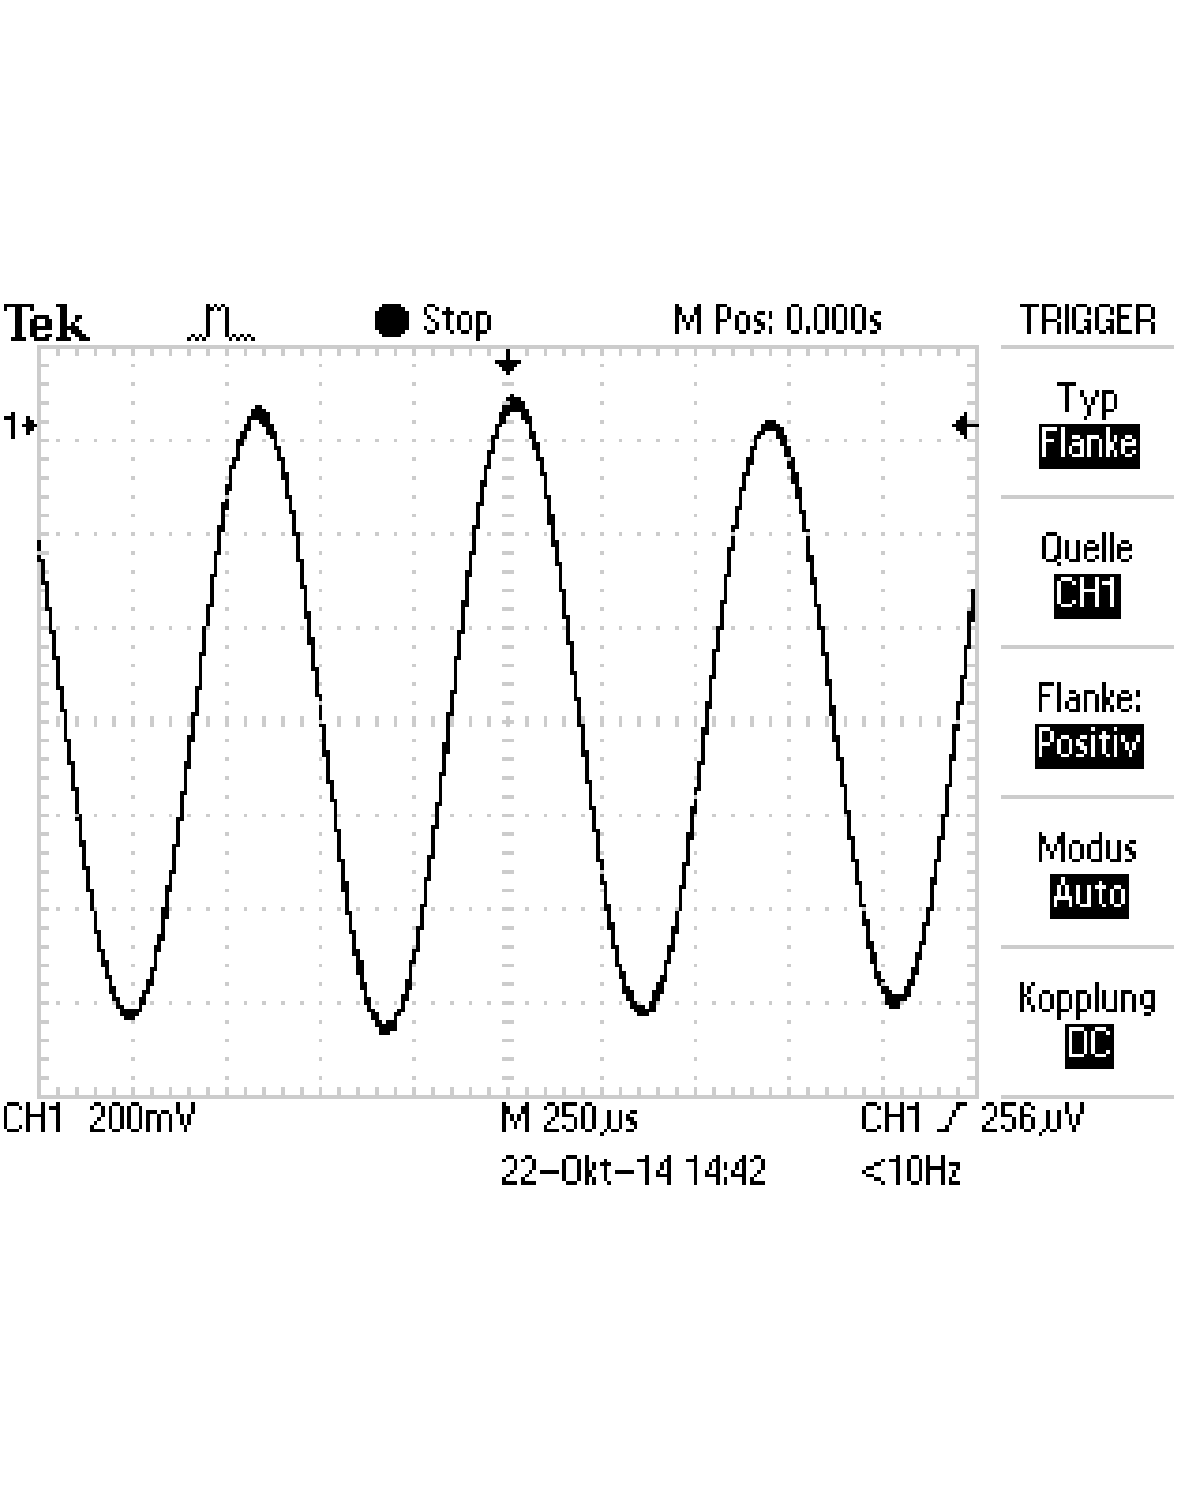
\includegraphics[width=\textwidth , scale = 0.4]{2_3_r3np_sig.pdf}
				\caption[Aufnahme des mit dem Mikrofon aufgenommenen Signals. R$_3$ ist nicht mit der Masse verbunden.]{Aufnahme des mit dem Mikrofon aufgenommenen Signals.R$_3$ ist nicht mit der Masse verbunden.}
  				\label{fig:2_3_r3np_sig}
        \end{subfigure}
       % ~ %add desired spacing between images, e. g. ~, \quad, \qquad, \hfill etc.
          %(or a blank line to force the subfigure onto a new line)
        \hfill
        \begin{subfigure}[tb]{0.48\textwidth}
                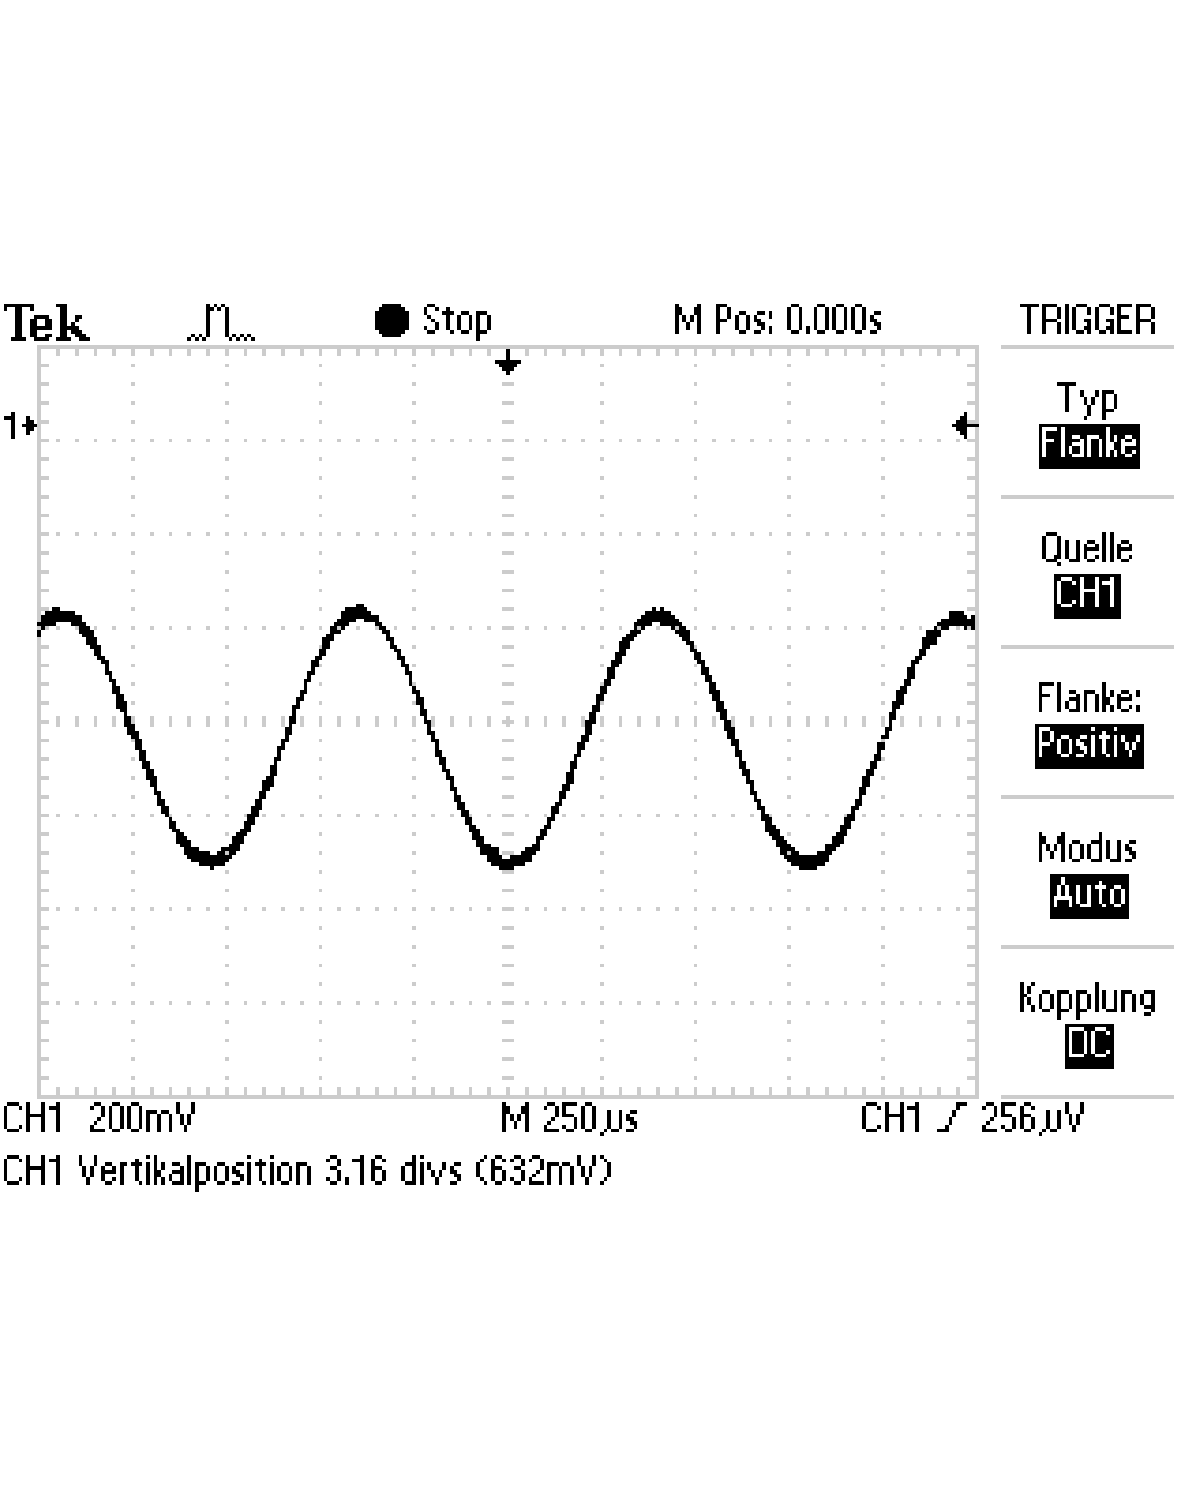
\includegraphics[trim = 0cm 0cm 0cm 3cm , clip , width=\textwidth , scale = 0.4]{2_3_r3p_sig.pdf}
                \caption[Abbildung des mit dem Mikrofon aufgenommenen Signals am Oszilloskop, R$_3$ parallel zu R$_4$ geschaltet]{Abbildung des mit dem Mikrofon aufgenommenen Signals, R$_3$ parallel zu R$_4$ geschaltet}
  				\label{fig:2_3_r3p_sig}
        \end{subfigure}
        \caption{Kurven der durch Pfeifen erzeugten Signale}
        \label{fig:2_3_sin_vergleich}
\end{figure}



Betrachtet man die Störung, die dadurch verursacht wird, dass man das Mikrofon auf den Funktionsgenerator legt, so erhält man für R$_3$ nicht parallel zu R$_4$ die Kurve in Abbildung \ref{fig:2_3_r3np_sig}. Für den Aufbau mit R$_3$ parallel zu R$_4$ ergibt sich die Kurve aus Abbildung \ref{fig:2_3_r3p_sig}. Wieder ist zu erkennen, dass die Verzerrung der Kurve aus Abbildung \ref{fig:2_3_r3p_st} größer ist als in Abbildung \ref{fig:2_3_r3np_st}.


\begin{figure}[H]
        \centering
        \begin{subfigure}[tb]{0.48\textwidth}
                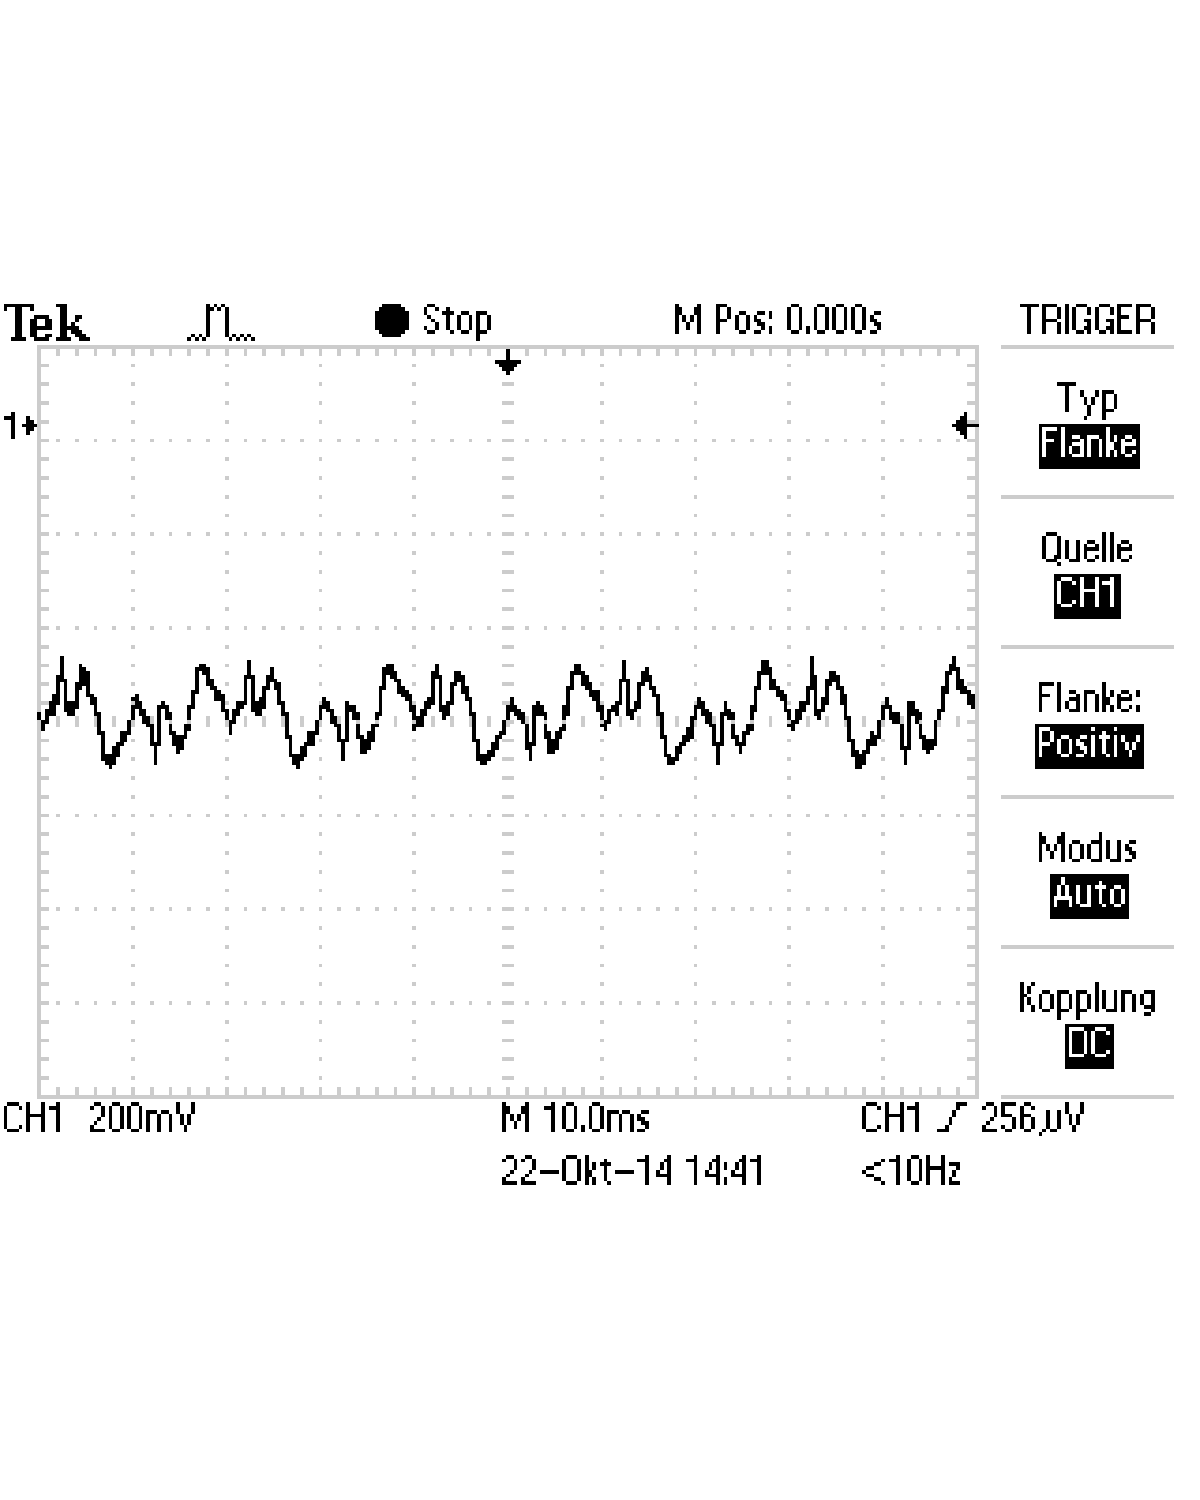
\includegraphics[width=\textwidth , scale = 0.4]{2_3_r3np_st.pdf}
				\caption[Aufnahme der mit dem Mikrofon aufgenommenen Störung.R$_3$ ist nicht mit der Masse verbunden.]{Aufnahme der mit dem Mikrofon aufgenommenen Störung.R$_3$ ist nicht mit der Masse verbunden.}
 	 			\label{fig:2_3_r3np_st}
        \end{subfigure}%
       % ~ %add desired spacing between images, e. g. ~, \quad, \qquad, \hfill etc.
          %(or a blank line to force the subfigure onto a new line)
        \hfill
        \begin{subfigure}[tb]{0.48\textwidth}
                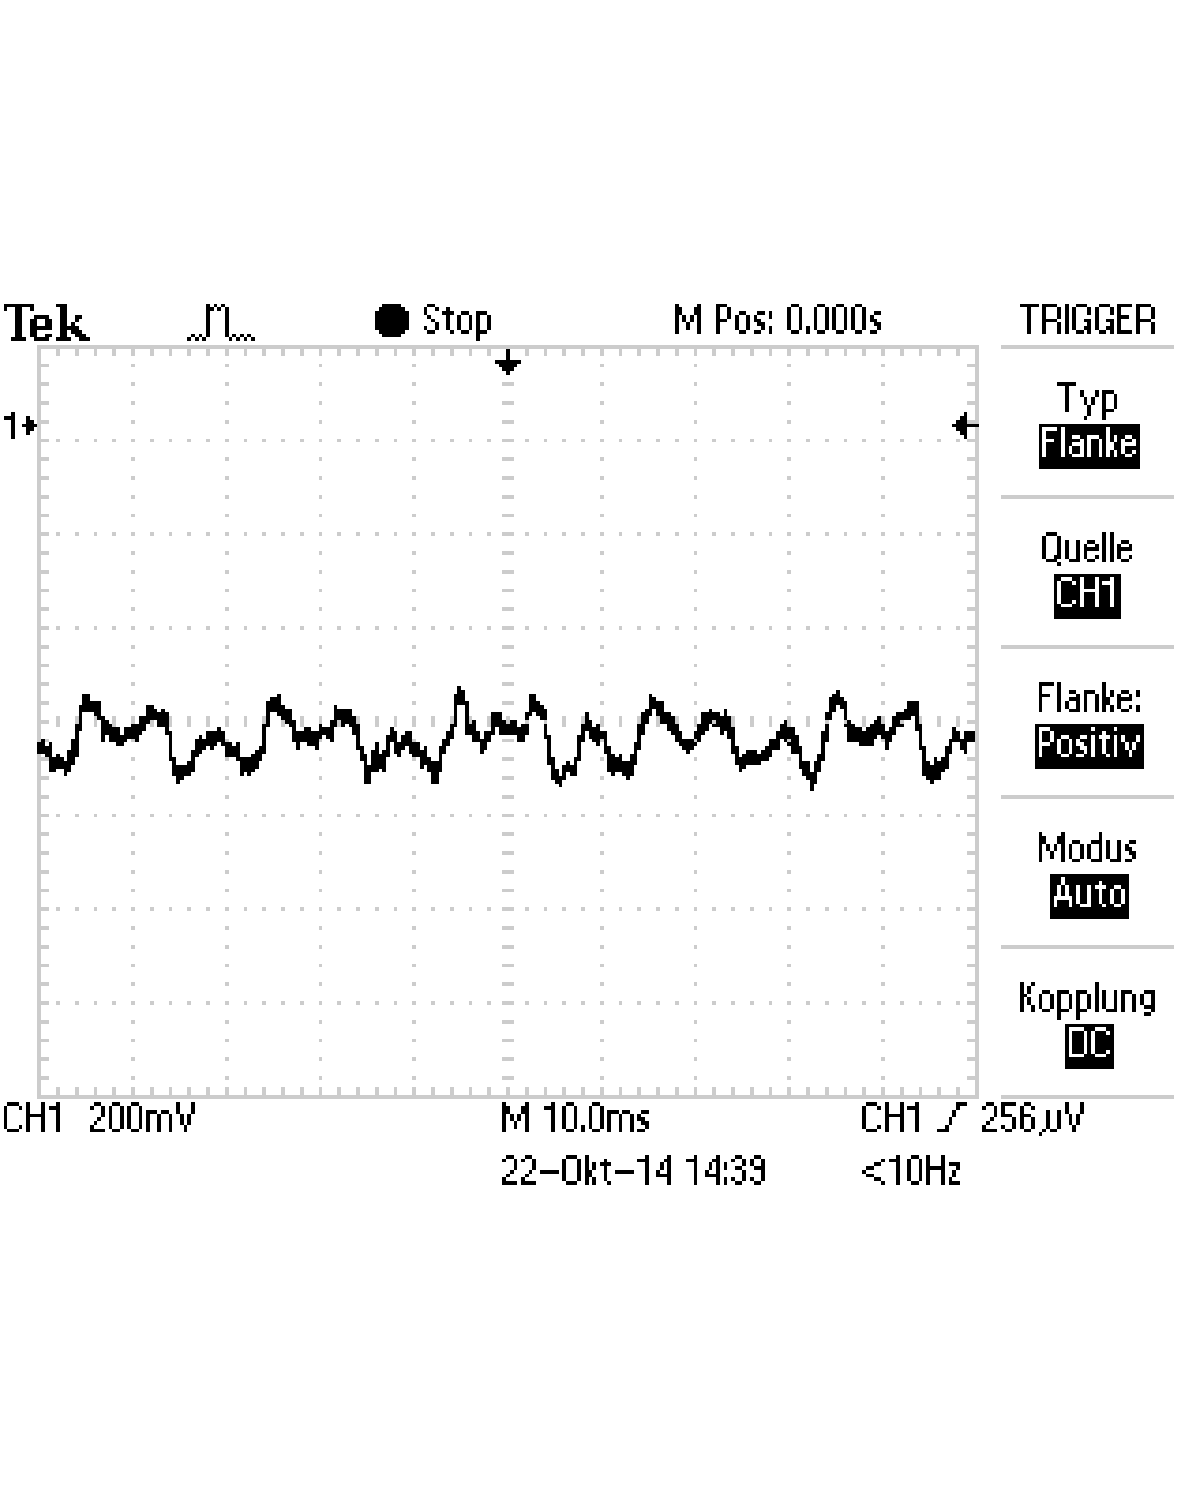
\includegraphics[width=\textwidth , scale = 0.4]{2_3_r3p_st.pdf}
                \caption[Aufnahme der mit dem Mikrofon aufgenommenen Störung, R$_3$ parallel zu R$_4$ geschaltet]{Aufnahme der mit dem Mikrofon aufgenommenen Störung, R$_3$ parallel zu R$_4$ geschaltet}
  				\label{fig:2_3_r3p_st}
        \end{subfigure}
        \caption{Kurve der Störung durch den Funktionsgenerator}
        \label{fig:2_2_stoer_vergleich}
\end{figure}



\subsection{Diskussion}
%(immer) die gemessenen werte und die bestimmten werte über die messfehler mit literaturwerten oder untereinander vergleichen
%in welchem fehlerintervall des messwertes liegt der literaturwert oder der vergleichswert?
%wie ist der relative anteil des fehlers am messwert und damit die qualität unserer messung?
%in einem satz erklären, wie gut unser fehler und damit unsere messung ist
%kurz erläutern, wie systematische fehler unsere messung beeinflusst haben könnten
%(wichtig) zum schluss ansprechen, in wie weit die ergebnisse mit der theoretischen vorhersage übereinstimmen
%--------------------------------------------------------------------------------------------
%falls tabellen mit den messwerten zu lang werden, kann die section mit den messwerten auch hinter der diskussion angefügt bzw. eine section mit dem anhang eingefügt werden.

Wie erwartet ergab sich bei der Verwendung von zwei Bananenkabeln im Gegensatz zu einem Bananenkabel nur eine leichte Verbesserung, da die Erdung von Funktionsgenerator und Oszilloskop jeweils nur einen geringen Gegenstrom zuließen (vgl Abbildung \ref{fig:2_1_rech_vergleich} und Abbildung \ref{fig:2_2_rech_vergleich}).
Da dies auch für die zwei verdrillten Bananenkabel gilt konnte kaum Verbesserung beobachtet werden, Abbildung \ref{fig:2_3_rech_vergleich_ohne_mikro}. Beim Verwenden des Mikrofons als Signalquelle ließ sich eine leichte Verbesserung feststellen, wenn R$_3$ nicht mit der Masse verbunden war, Abbildung \ref{fig:2_3_sin_vergleich} und Abbildung \ref{fig:2_2_stoer_vergleich}.


\section{Signalübertragung über Koaxialkabel}
%kurz das ziel dieses versuchsteiles ansprechen, damit keine zwei überschriften direkt übereinander stehen!
%bei schwierigeren versuchen kann auch der theoretische hintergrund erläutert werden. (mit formeln, herleitungen und erklärungen)

In diesem Versuchsabschnitt werden die Signalübertragungseigenschaften von Koaxialkabeln untersucht.

\subsection{Versuchsaufbau}
%skizze zum versuchsaufbau (oder foto) einfügen,   es muss erklärt werden wie das ganze funktioniert und welche speziellen einstellungen verwendet wurden (z.b. welche knöpfe an den geräten für die messung verdreht wurden)

In diesem Abschnitt werden die 5 Versuchsaufbauten skizziert.

\subsubsection{Kurzes Koaxialkabel ohne Abschlußwiderstand}

Der Funktionsgenerator und das Oszilloskop werden mit einem Kurzem Koaxialkabel verbunden.

\begin{figure}[H] 
  \centering
    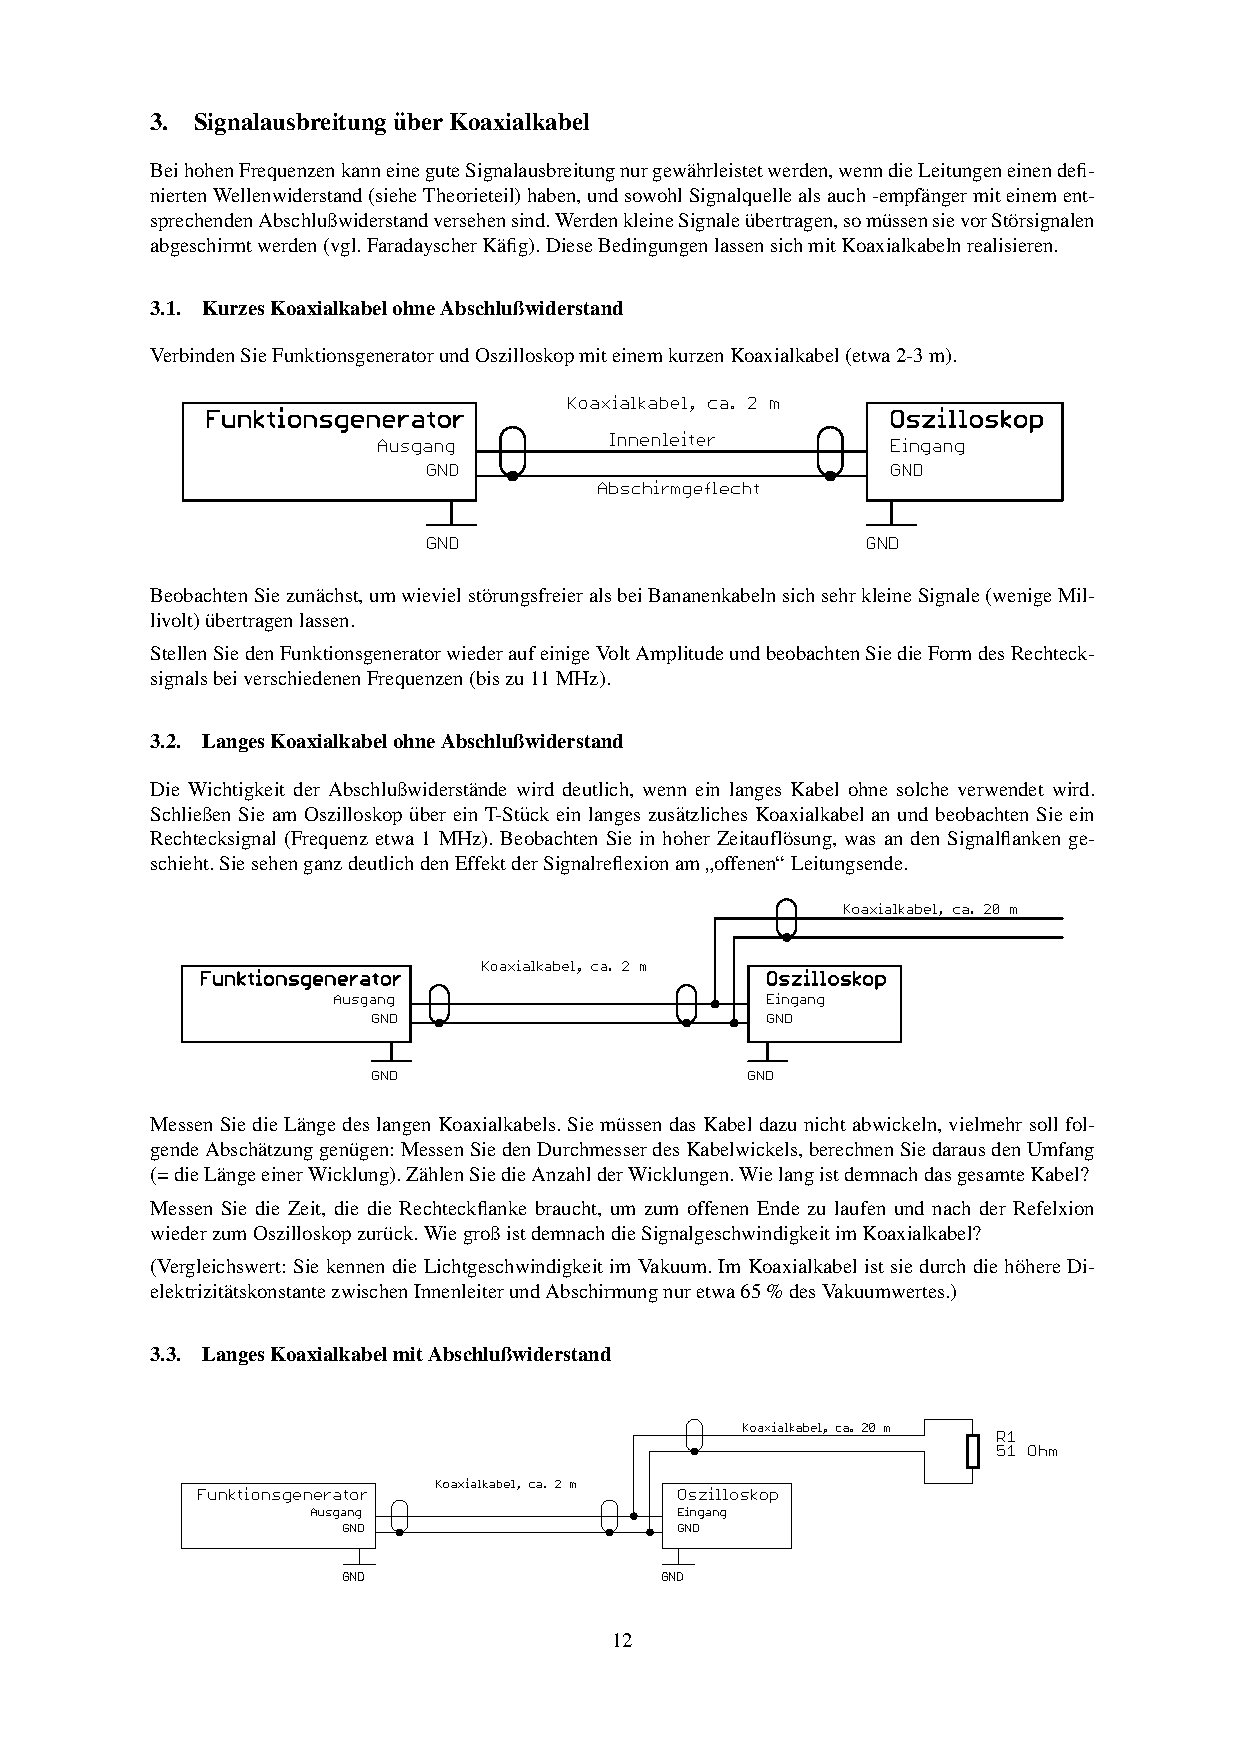
\includegraphics[trim = 10mm 200mm 10mm 65mm, clip, scale = 1]{3-3_3.pdf}
  	\caption[Schaltskizze einer Verbindung zwischen Funktionsgenerator und Oszilloskop, mit kurzem Koaxialkabel]{Schaltskizze einer Verbindung zwischen Funktionsgenerator und Oszilloskop, mit kurzem Koaxialkabel\footnotemark}
  \label{fig:3.1}
\end{figure}
\footnotetext{Abbildung entnommen von http://www.atlas.uni-wuppertal.de/$\sim$kind/ep1\_14.pdf Seite 12 am 19.10.2014}

\subsubsection{Langes Koaxialkabel ohne Abschlußwiderstand}

Der Funktonsgenerator und das Oszilloskop werden mit einem kurzen Koaxialkabel verbunden, wobei ein langes Koaxialkabel mit offenem Ende über ein T-Verbindungsstück angeschlossen wird.

\begin{figure}[H] 
  \centering
    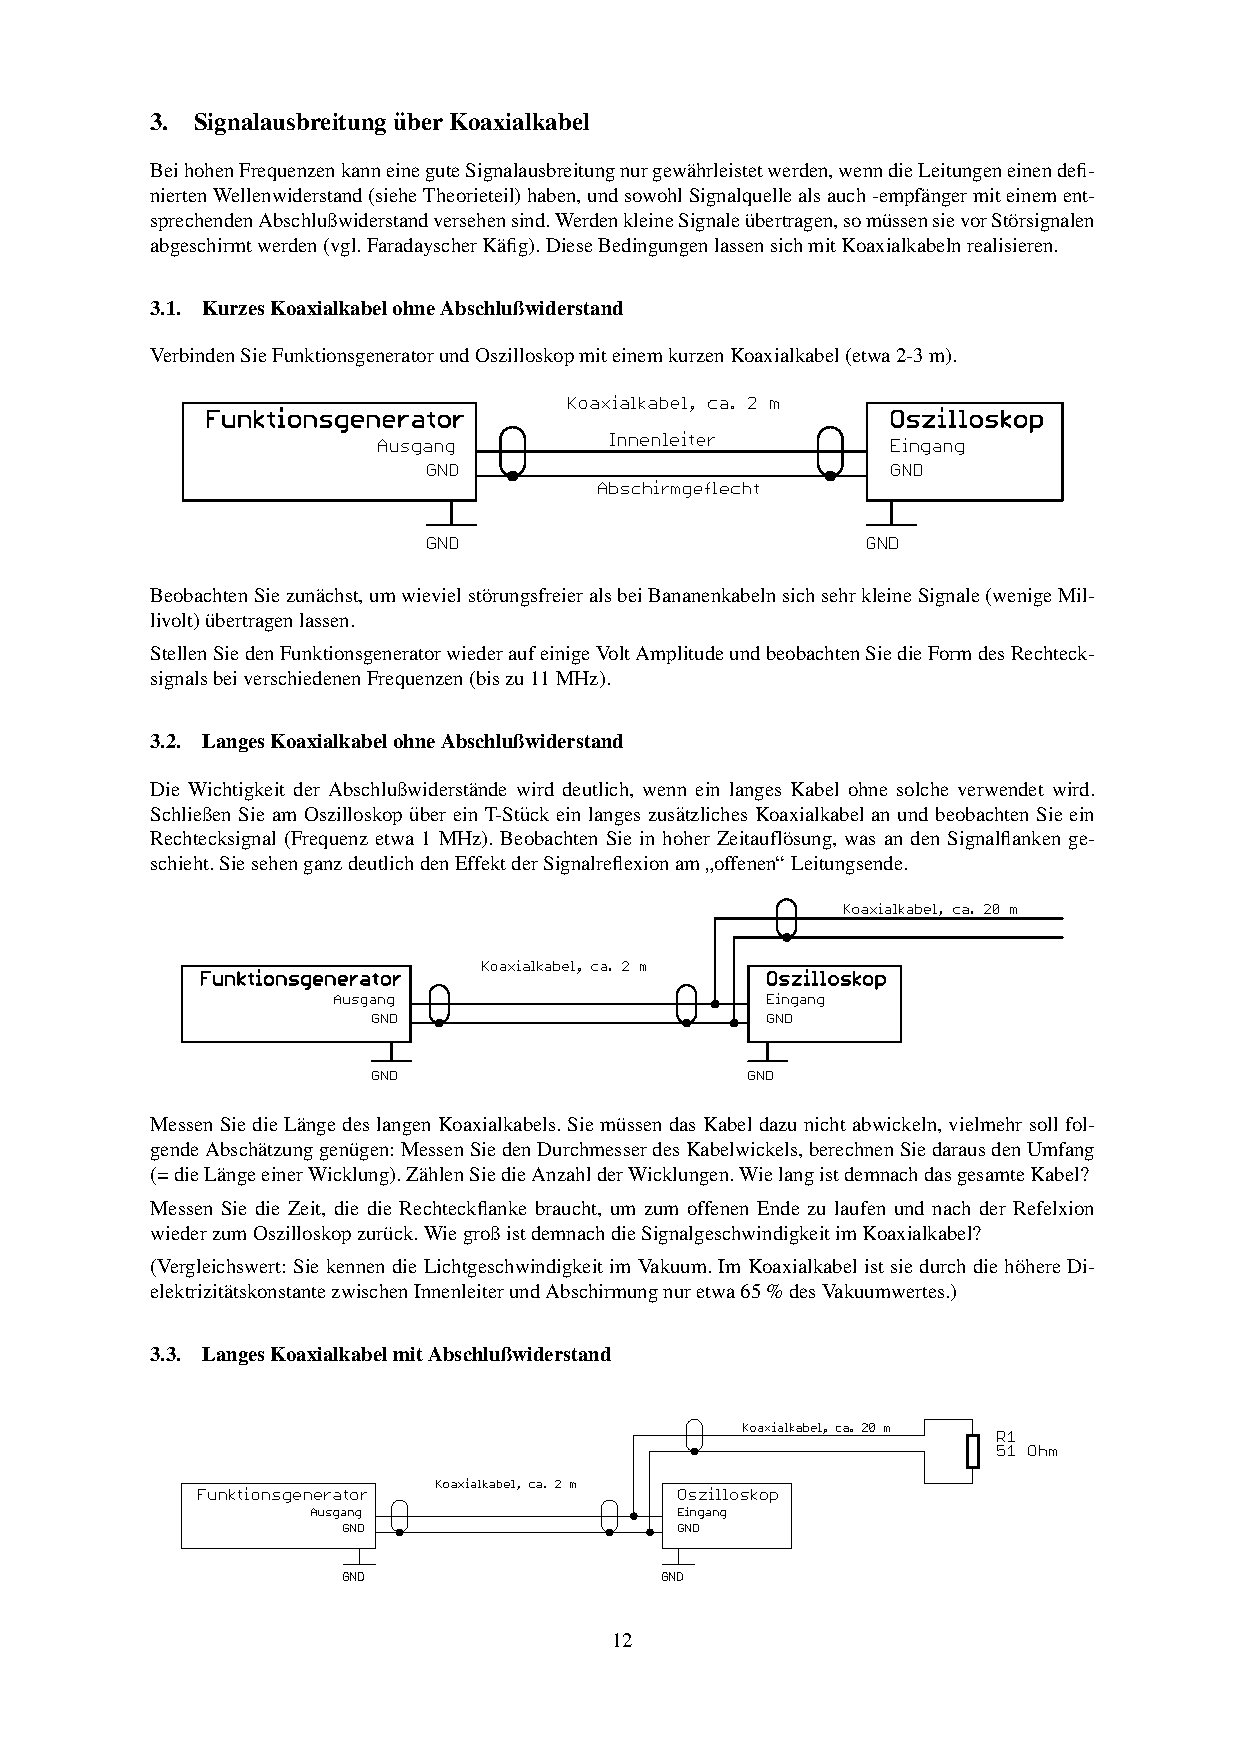
\includegraphics[trim = 10mm 110mm 10mm 150mm, clip, scale = 1]{3-3_3.pdf}
  	\caption[Schaltskizze einer Verbindung zwischen Funktionsgenerator und Oszilloskop, mit langem Koaxialkabel]{Schaltskizze einer Verbindung zwischen Funktionsgenerator und Oszilloskop, mit langem Koaxialkabel\footnotemark}
  \label{fig:3.2}
\end{figure}
\footnotetext{Abbildung entnommen von http://www.atlas.uni-wuppertal.de/$\sim$kind/ep1\_14.pdf Seite 12 am 19.10.2014}

\subsubsection{Langes Koaxialkabel mit Abschlußwiderstand}

Der Funktonsgenerator und das Oszilloskop werden mit einem kurzen Koaxialkabel verbunden, wobei ein langes Koaxialkabel mit Abschlusswiderstand am Ende über ein T-Verbindungsstück angeschlossen wird.

\begin{figure}[H] 
  \centering
    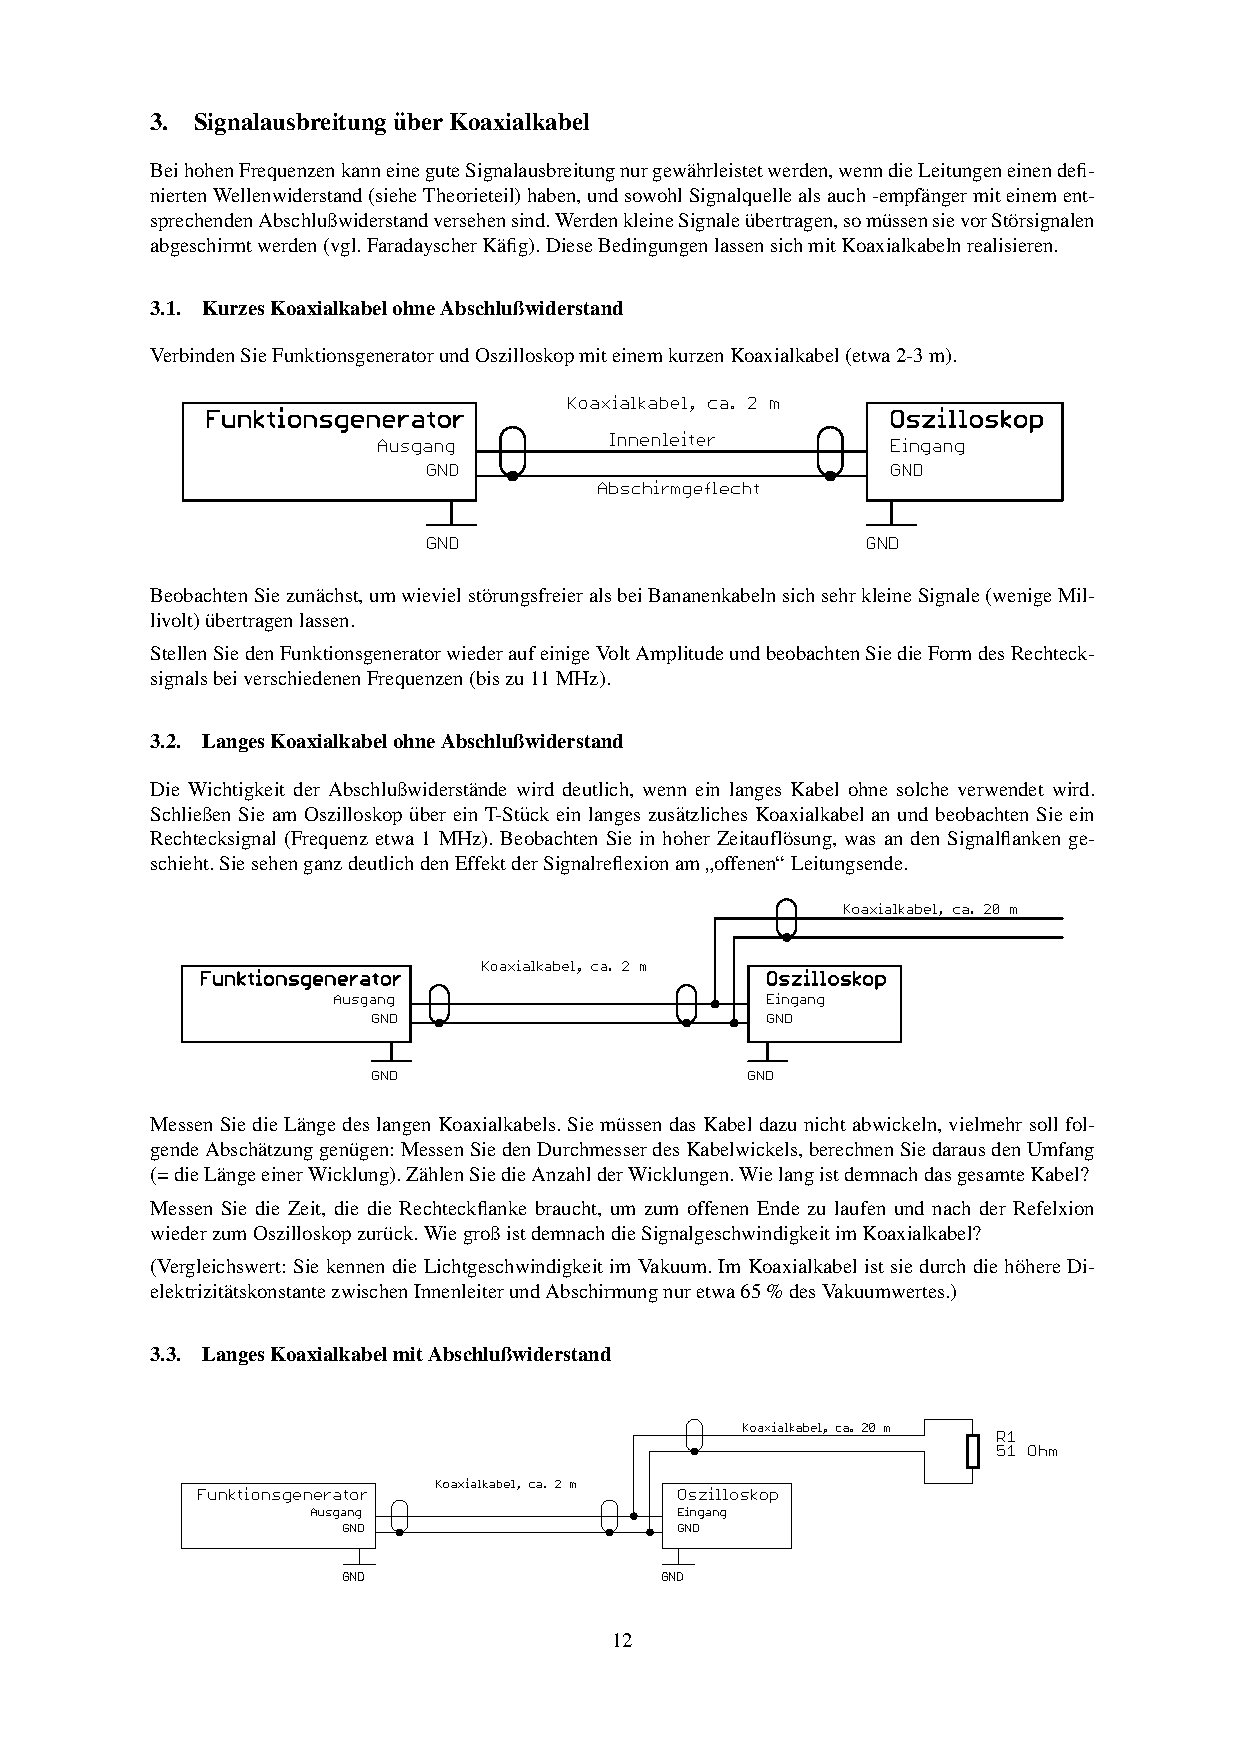
\includegraphics[trim = 10mm 25mm 10mm 235mm, clip, scale = 1]{3-3_3.pdf}
  	\caption[Schaltskizze einer Verbindung zwischen Funktionsgenerator und Oszilloskop, mit langem Koaxialkabel und Abschlusswiderstand]{Schaltskizze einer Verbindung zwischen Funktionsgenerator und Oszilloskop, mit langem Koaxialkabel und Abschlusswiderstand\footnotemark}
  \label{fig:3.3}
\end{figure}
\footnotetext{Abbildung entnommen von http://www.atlas.uni-wuppertal.de/$\sim$kind/ep1\_14.pdf Seite 12 am 19.10.2014}

\subsubsection{Langes Koaxialkabel mit Kurzschluß am Ende}

Der Funktonsgenerator und das Oszilloskop werden mit einem kurzen Koaxialkabel verbunden, wobei ein langes Koaxialkabel mit Kurzschluss am Ende über ein T-Verbindungsstück angeschlossen wird.

\begin{figure}[H] 
  \centering
    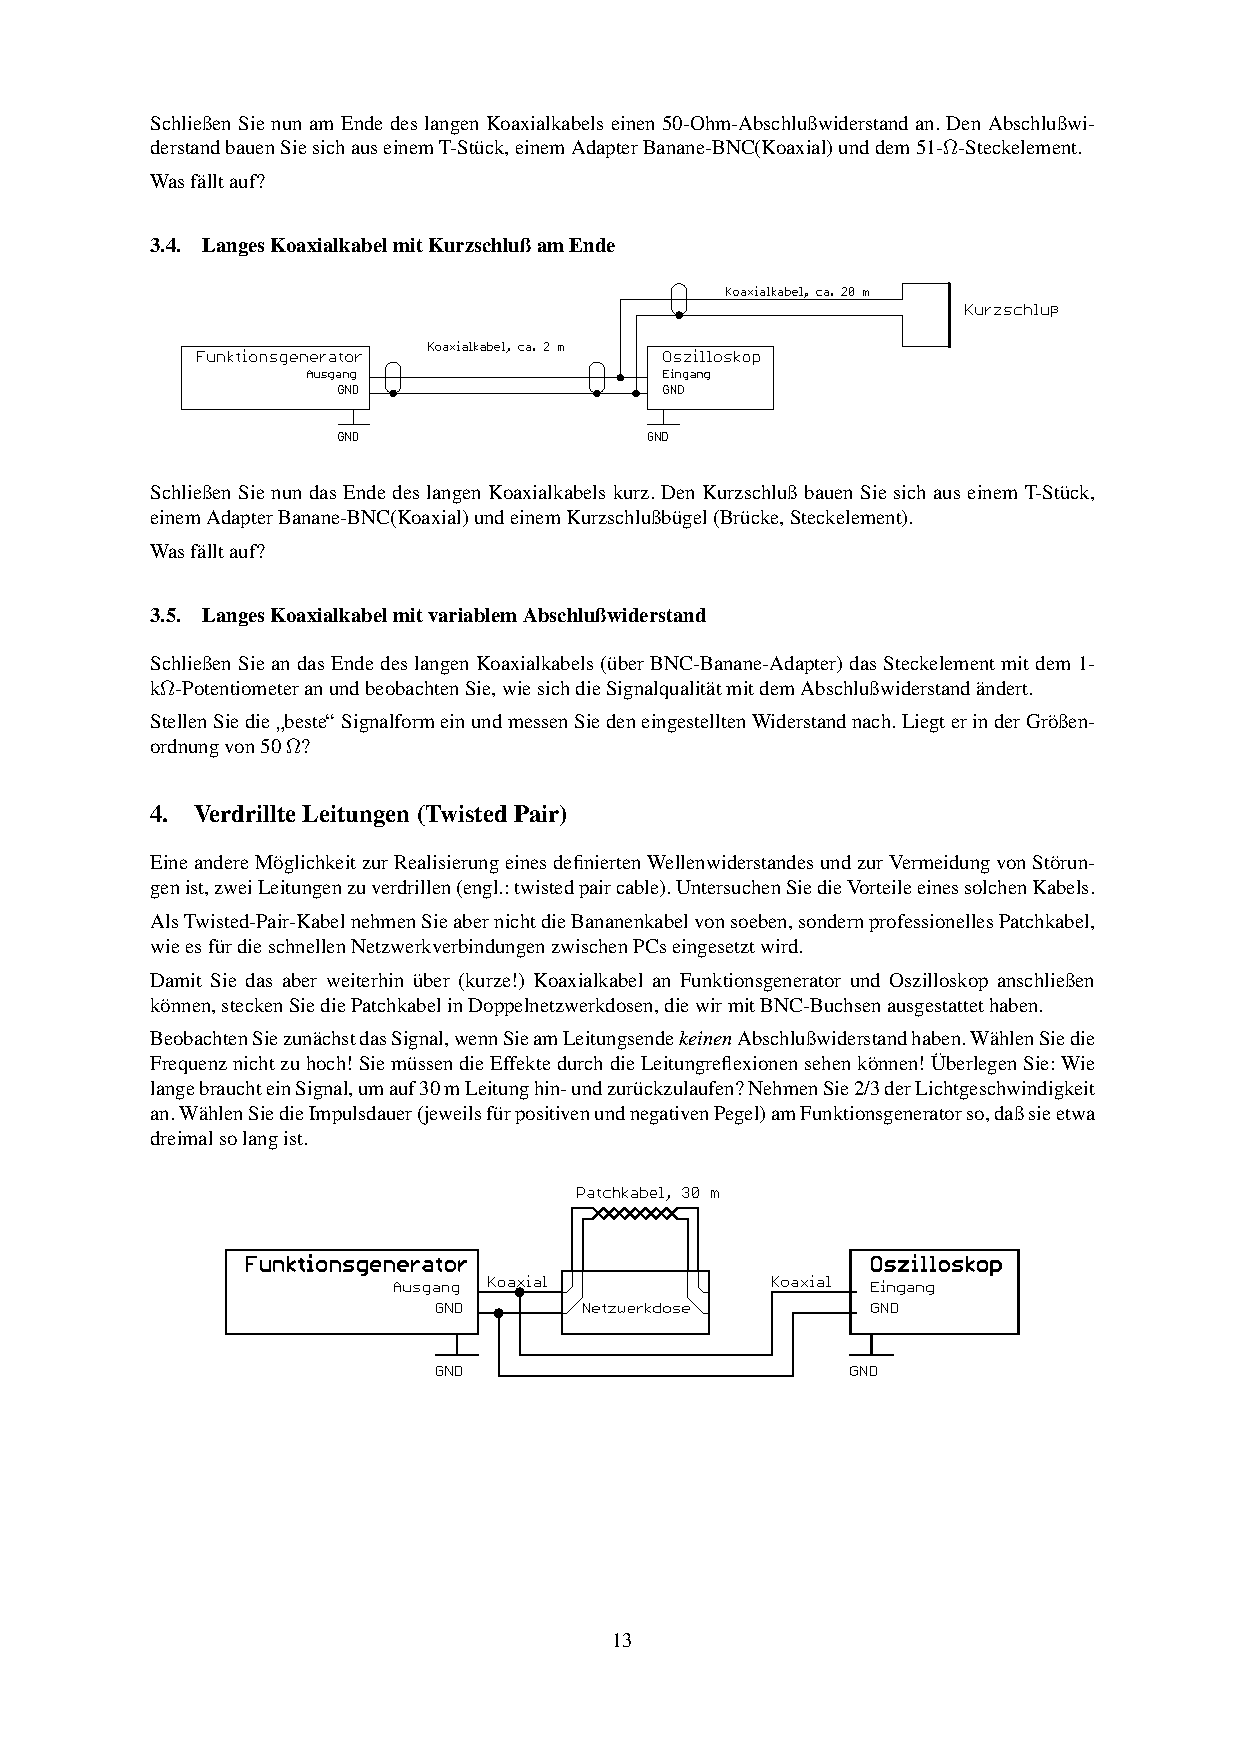
\includegraphics[trim = 10mm 220mm 10mm 45mm, clip, scale = 1]{3_4-4.pdf}
  	\caption[Schaltskizze einer Verbindung zwischen Funktionsgenerator und Oszilloskop, mit langem Koaxialkabel und Kurzschluss]{Schaltskizze einer Verbindung zwischen Funktionsgenerator und Oszilloskop, mit langem Koaxialkabel und Kurzschluss\footnotemark}
  \label{fig:3.4}
\end{figure}
\footnotetext{Abbildung entnommen von http://www.atlas.uni-wuppertal.de/$\sim$kind/ep1\_14.pdf Seite 13 am 19.10.2014}

\subsubsection{Langes Koaxialkabel mit variablem Abschlußwiderstand}

Der Funktonsgenerator und das Oszilloskop werden mit einem kurzen Koaxialkabel verbunden, wobei ein langes Koaxialkabel mit einem variablem Abschlusswiderstand am Ende über ein T-Verbindungsstück angeschlossen wird.

\begin{figure}[H] 
  \centering
    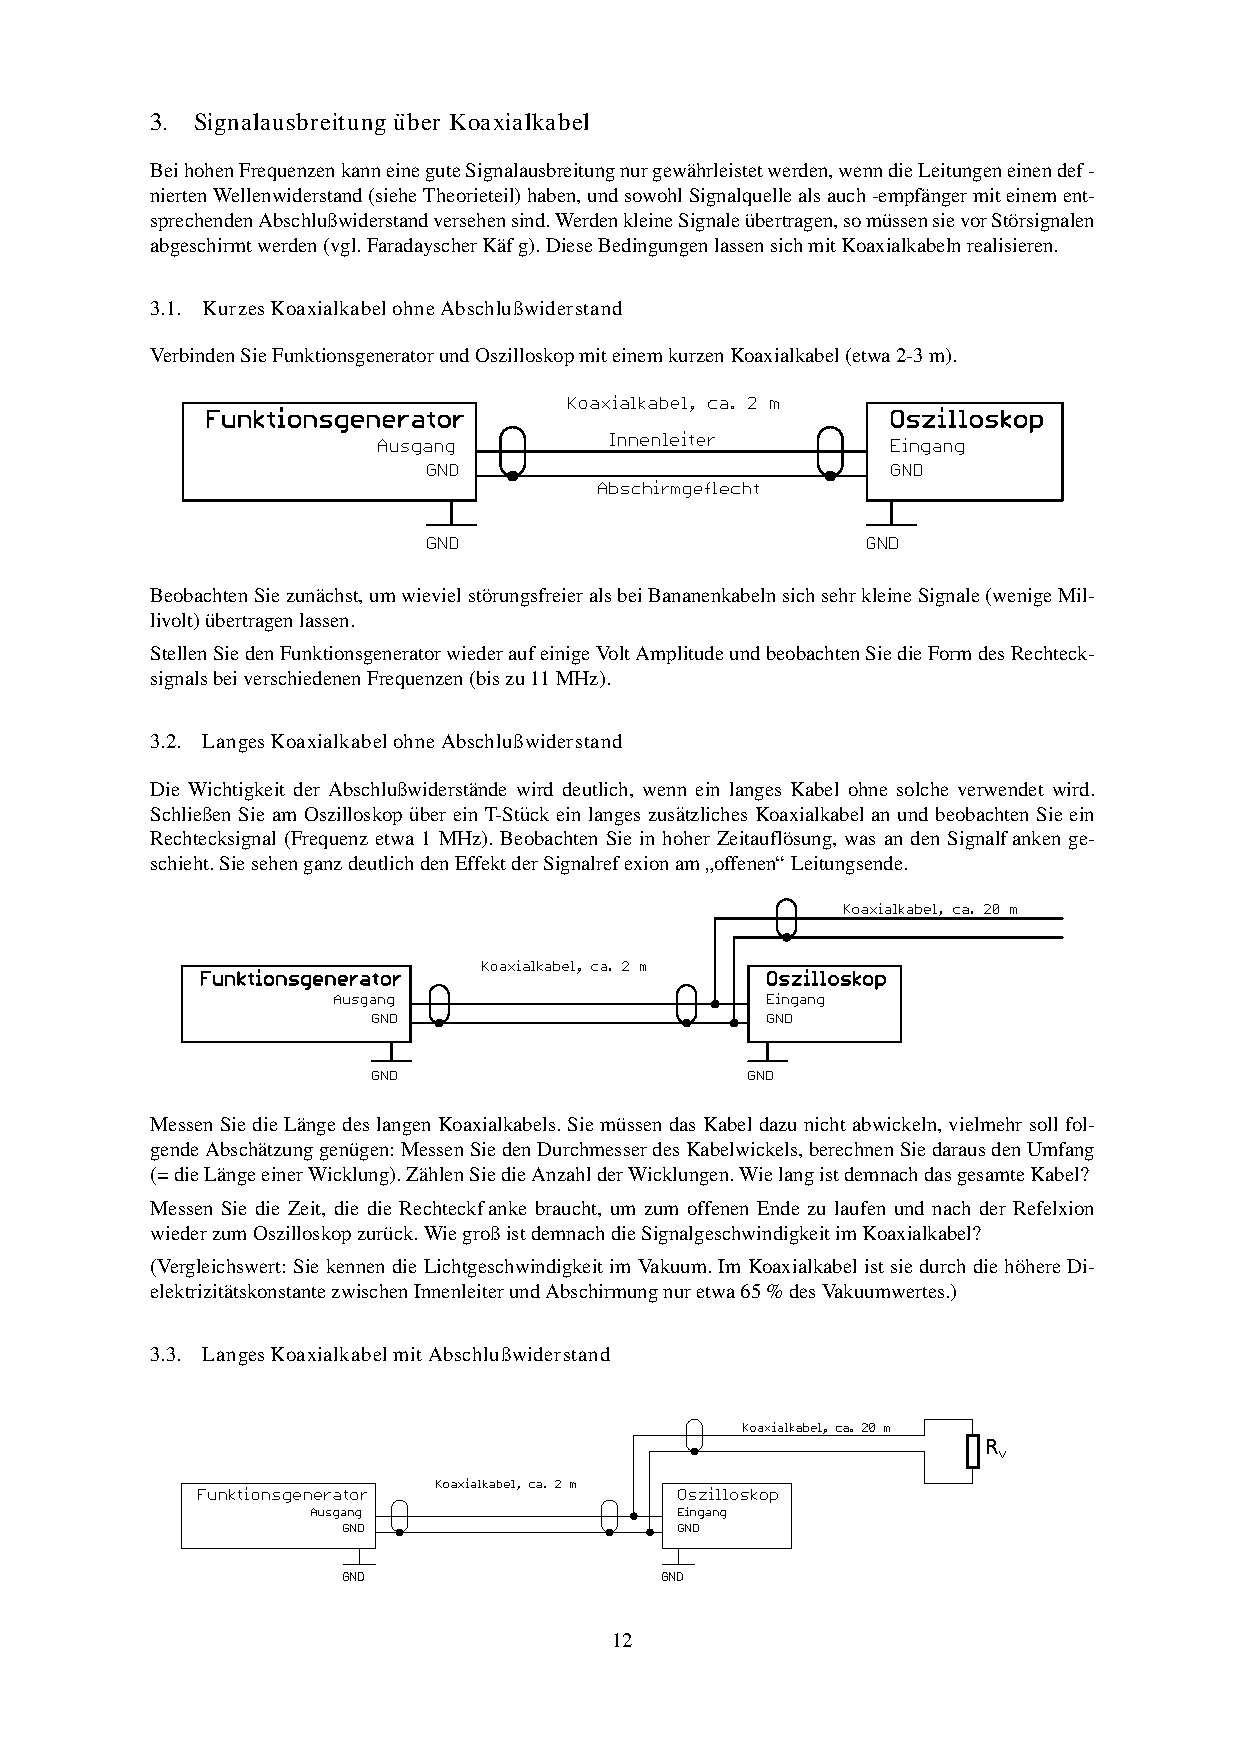
\includegraphics[trim = 10mm 25mm 10mm 235mm, clip, scale = 1]{3-3_3+1.pdf}
  	\caption[Schaltskizze einer Verbindung zwischen Funktionsgenerator und Oszilloskop, mit langem Koaxialkabel und variablem Abschlusswiderstand]{Schaltskizze einer Verbindung zwischen Funktionsgenerator und Oszilloskop, mit langem Koaxialkabel und variablem Abschlusswiderstand\footnotemark}
  \label{fig:3.5}
\end{figure}
\footnotetext{Abbildung entnommen von http://www.atlas.uni-wuppertal.de/$\sim$kind/ep1\_14.pdf Seite 12 am 19.10.2014}

\subsection{Versuchsdurchführung}
%erklären, !was! wir machen, !warum! wir das machen und mit welchem ziel
%(wichtig) präzize erklären, wie bei dem versuch vorgegangen und was gemacht wurde
In Aufgabe 3.1 wurde der Funktionsgenerator über ein 2m langes Koaxialkabel mit dem Oszilloskop verbunden. Der Unterschied der Qualität der Signalübertragung zwischen Koaxialkabel und Bananenkabel wird bei kleinen Amplituden und verschiedenen Frequenzen untersucht.
In Aufgabe 3.2 wird über ein T-Stück ein langes Koaxialkabel an das Oszilloskop angeschlossen. Die Länge des Kabels bestimmt man über den Durchmesser und die Anzahl der Wicklungen, um nicht das gesamte Kabel abrollen zu müssen. Das am Oszilloskop angezeigte Rechtecksignal wird von dem am offenen Ende des Kabels reflektierten Signal nach zweimaligem Durchlaufen überlagert, sodass ein Teil der rechten Flancke des reflektierten Signals sich mit dem nachfolgenden Signal weghebt. Die Breite dieser Flancke entspricht dann der Laufzeit des Signals durch das Koaxialkabel (als Vergleichswert wurde eine Phasengeschwindigkeit von $\frac{2}{3}C_0$ angenommen).
In Aufgabe 3.3 wird ein \unit[50]{$\Omega$} Widerstand an das lange Koaxialkabel angeschlossen und der Effekt auf die Reflektion des Signals mit dem Ergebnis aus dem zweiten Teil verglichen.
In Aufgabe 3.4 soll das Koaxialkabel kurzgeschlossen werden. Da durch den Kurzschluss ein Knotenpunkt der Spannung erzeugt wird, wird das Signal mit umgekehrtem Vorzeichen reflektiert. Das Ergebnis kann mit den beiden Aufgabenteilen davor verglichen werden.
In Aufgabe 3.5 wird nochmal ein Potentiometer von 0 bis \unit[1]{k$\Omega$} an das Koaxialkabel angeschlossen, um den Wellenwiderstand des Kabels, bei dem kein Signal zurückgeworfen wird von Hand zu bestimmen. Die Reflektion kann bei eingestelltem Rechtecksignal am Oszilloskop beobachtet werden.


\subsection{Auswertung}
%zuerst !alle! errechneten werte entweder in ganzen sätzen aufzählen, oder in tabellen (übersichtlicher) dargestellen, sowie auf die verwendeten formeln verweisen (die referenzierung der formel kann in der überschrift stehen)
%kurz erwähnen (vor der tabelle), warum wir das ganze ausrechnen bzw. was wir dort ausrechnen
%danach histogramme und plots erstellen, wobei wenn möglich funktionen durch die plots gelegt werden (zur not können auch splines benutzt werden, was aber angegeben werden muss)
%bei fits immer die funktion und das reduzierte chiquadrat mit angegeben, wobei auf verständlichkeit beim entziffern der zehnerpotenzen geachtet werden muss z.b. f(x)=(wert+-fehler)\cdot10^{irgendeine zahl}\cdot x + (wert+-fehler)\cdot10^{irgendeine zahl}
%bei jedem fit erklären, nach welchem zusammenhang gefittet wurde und warum!
%bei plots darauf achten, dass die achsenbeschriftung (auch die tics) die richtige größe haben und die legende im plot nicht die messwerte verdeckt
%kurz die aufgabenstellung abgehandeln

In der Auswertung wird das Signal in Abhängigkeit des Abschlusses untersucht.

\subsubsection{Kurzes Koaxialkabel ohne Abschlußwiderstand}
Im ersten Versuchsteil sollte überprüft werden wie gut Rechtecksignale mit kleinen Amplituden von Koaxialkabeln übertragen werden. Dabei ergeben sich die Kurven in Abbildung \ref{fig:3_1_vergleich}. Es ist deutlich zu sehen, dass das Rechtecksignal bei 10MHz besser übertragen wird als bei Bananenkabeln, vgl. Abbildung \ref{fig:2_2_rech_10mhz}.

\begin{figure}[H]
        \centering
        \begin{subfigure}[tb]{0.48\textwidth}
                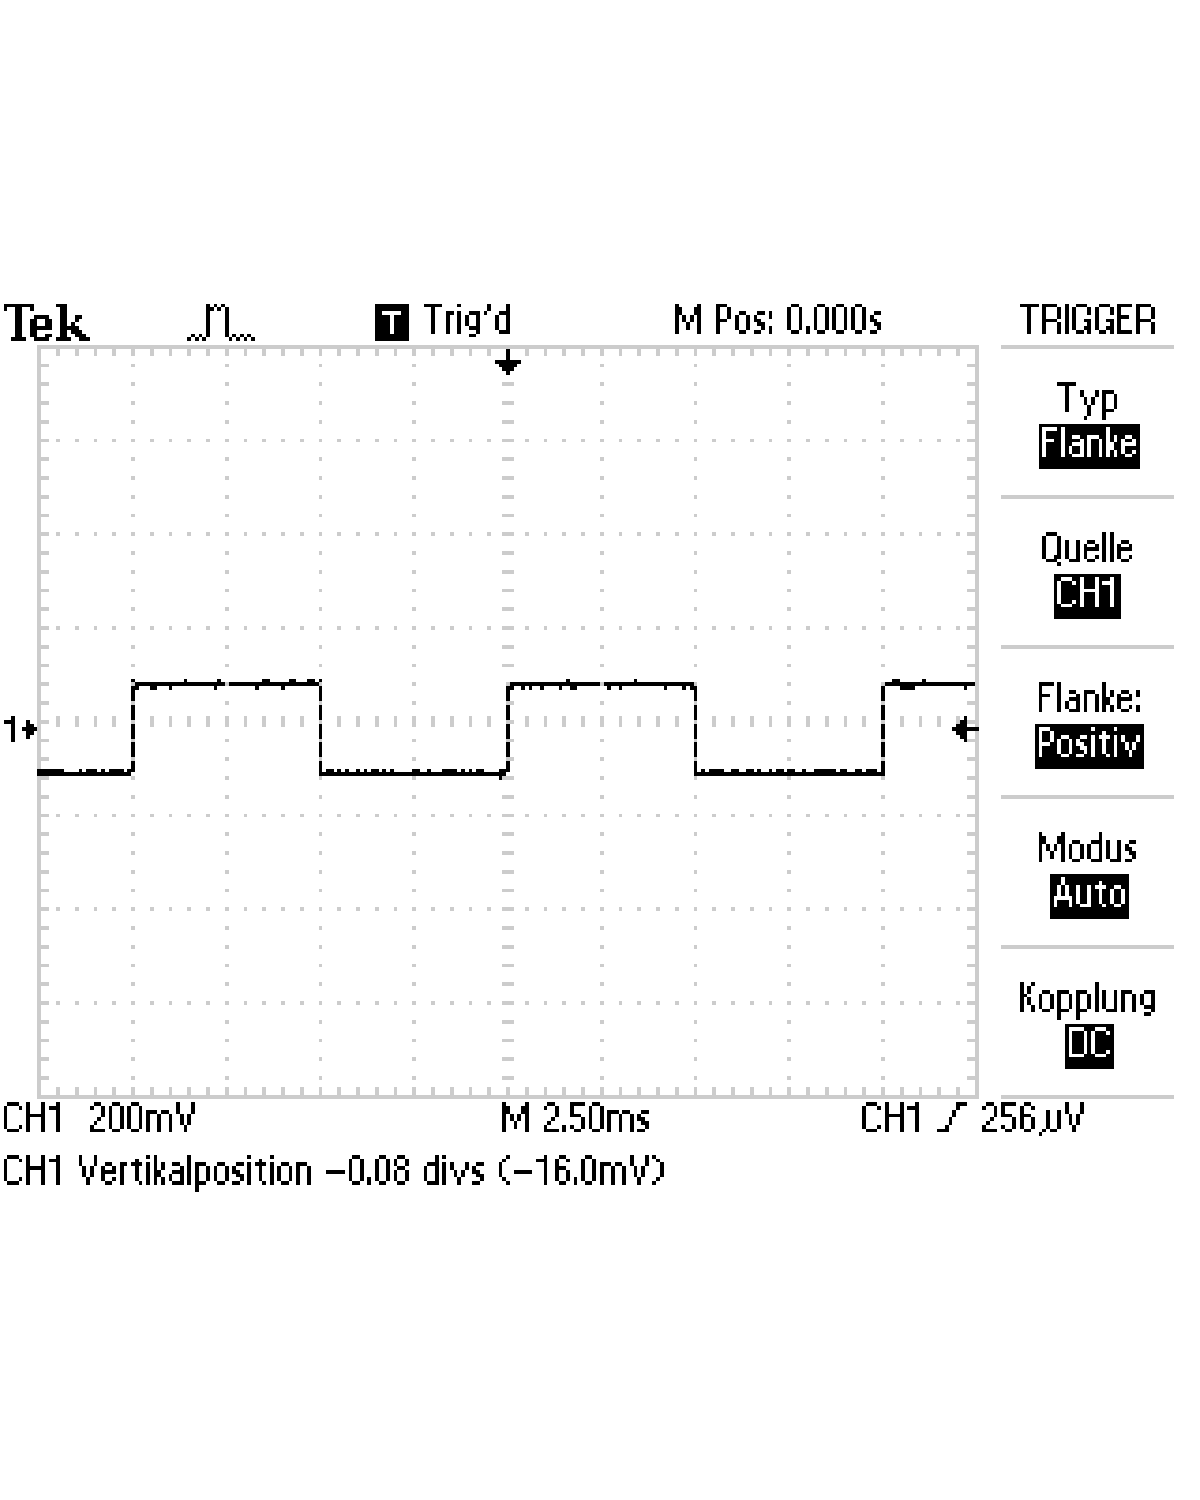
\includegraphics[width=\textwidth , scale = 0.4]{3_1_100hz.pdf}
				\caption[Aufnahme des Rechtecksignals für 100hz]{Aufnahme des Rechtecksignals für 100hz}
 	 			\label{fig:3_1_100hz}
        \end{subfigure}%
        ~ %add desired spacing between images, e. g. ~, \quad, \qquad, \hfill etc.
          %(or a blank line to force the subfigure onto a new line)
        \hfill
        \begin{subfigure}[tb]{0.48\textwidth}
                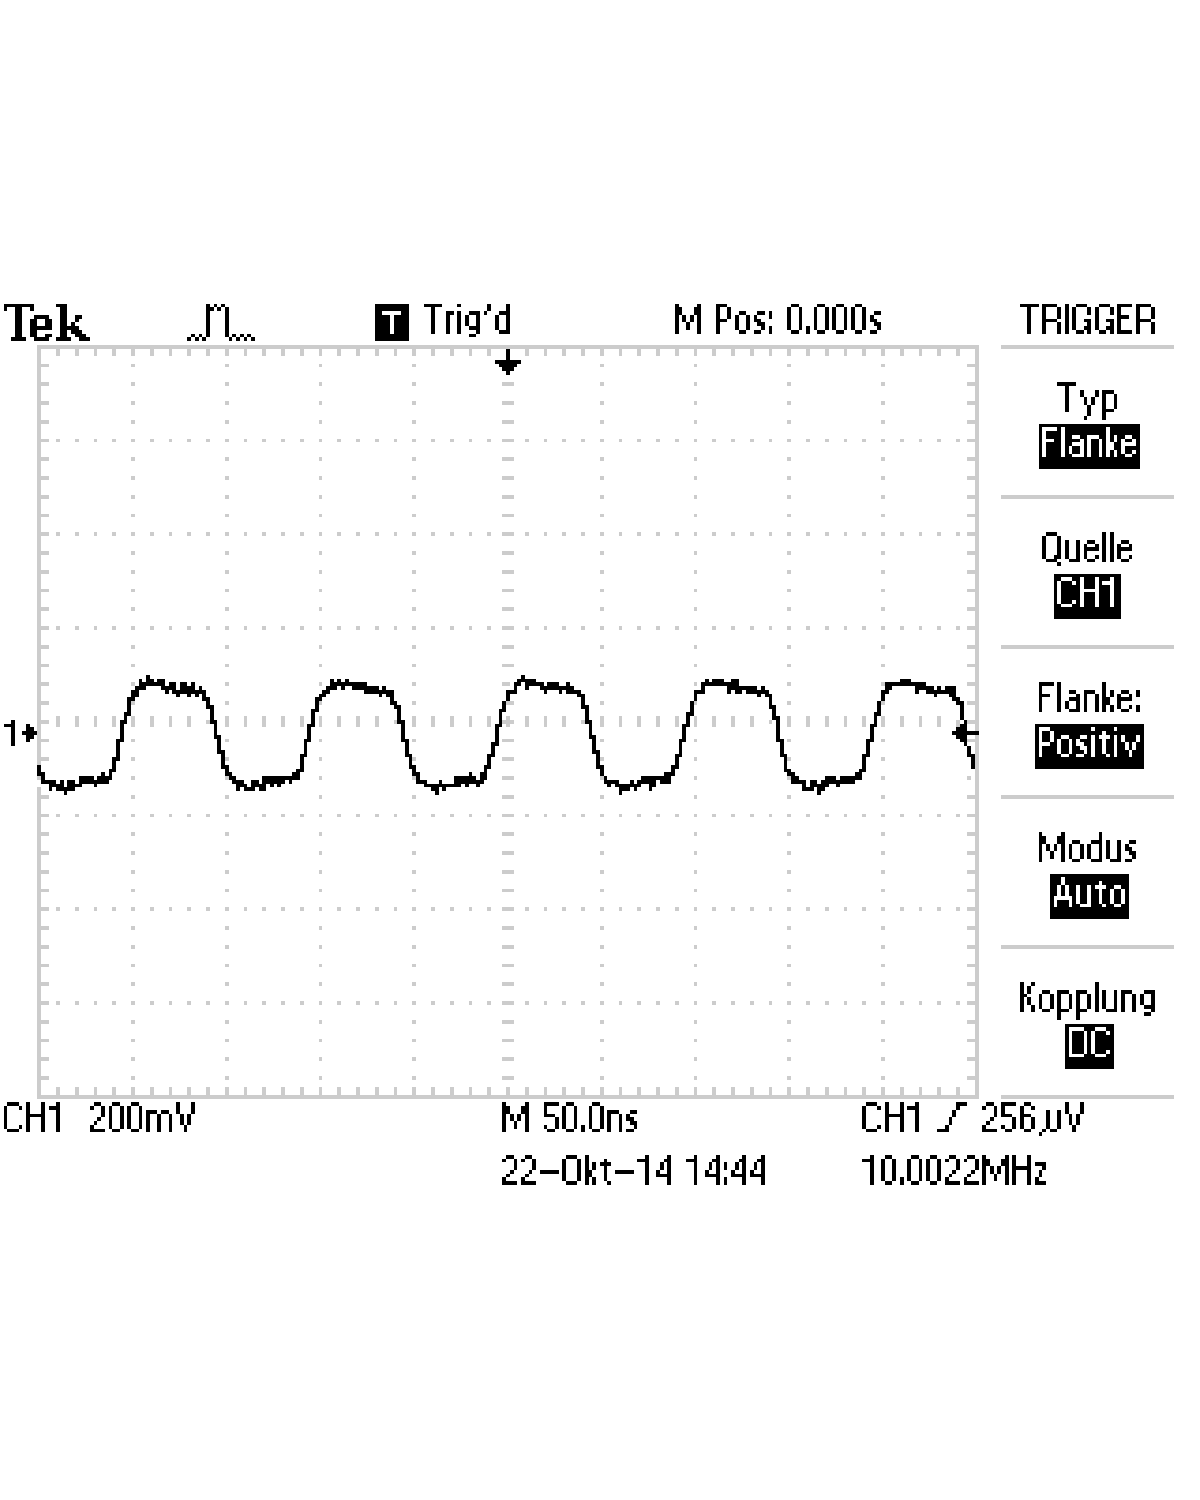
\includegraphics[width=\textwidth , scale = 0.4]{3_1_10mhz.pdf}
                \caption[Aufnahme des Rechtecksignals für 10Mhz]{Aufnahme des Rechtecksignals für 10Mhz}
  				\label{fig:3_1_mhz}
        \end{subfigure}
        \caption{Kurve des Rechtecksignals bei Übertragung mit einem Rechtecksignal bei kleinen Amplituden}
        \label{fig:3_1_vergleich}
\end{figure}



\subsubsection{Langes Koaxialkabel ohne Abschlußwiderstand}

Im zweitem Versuchsteil sollte aus der Länge des Kabels und der Durchlaufzeit des Signals durch das offene Koaxialkabel die Signalgeschwindigkeit bestimmt werden. Die Länge des Kabels wurde über den Durchmesser und die Windungszahl mit \unit[11,5 $\pm 0,5$]{m} bestimmt. Die Durchlaufzeit wurde aus der auf dem Oszilloskop angezeigten Kurve aus der Rechteckflanke bestimmt, Abbildung \ref{fig:3_2}. Es wurde ein Wert von \unit[120 $\pm10$]{ns} gemessen, daraus ergibt sich eine Signalgeschwindigkeit von \unit[(1,916 $\pm 0,02$ ) $\cdot 10^9$]{$\frac{\text{m}}{\text{s}}$}. Die Signalgeschwindigkeit wurde dabei mit 

\begin{align}
\text{v}_\text{Signal} = \frac{2 \cdot \text{l}_\text{Kabel}}{\text{t}_\text{Durchlaufzeit}}
\end{align}

bestimmt und der Fehler durch Fehlerfortpflanzung

\begin{align}
\Delta \text{v}_\text{Signal} = \sqrt{\left( \frac{2 \Delta \text{l}}{\text{t}} \right)^2 + \left( \frac{2 \text{l} \Delta \text{t}}{\text{t}^2} \right)^2}
\end{align}

\begin{figure}[H] 
  \centering
    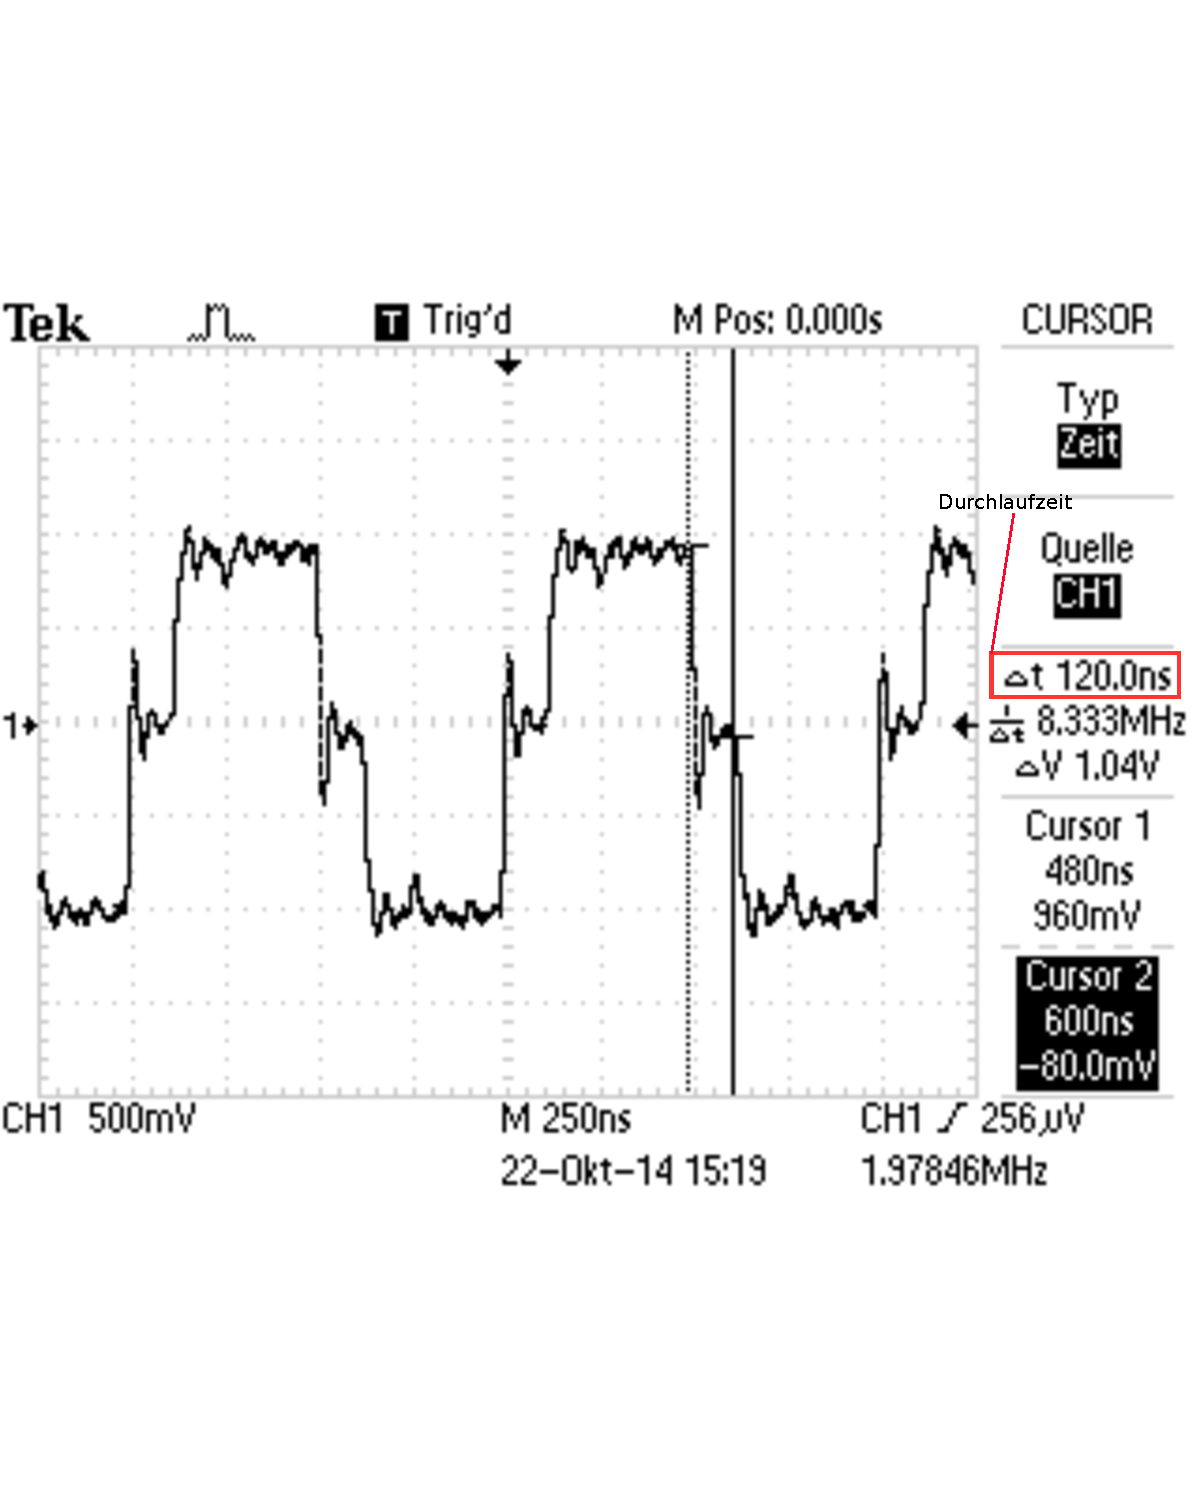
\includegraphics[scale = 0.5]{3_2.pdf}
  	\caption[Aufnahme des Signals bei 2MHz]{Aufnahme des Signals bei 2MHz}
  \label{fig:3_2}
\end{figure}

\subsubsection{Langes Koaxialkabel mit Abschlußwiderstand}

Im dritten Versuchsteil sollte das Koaxialkabel mit einem 51$\Omega$ Widerstand abgeschlossen werden. Es sollte beobachtet werden wie sich das Übertragene Signal ändert. In Abbildung \ref{fig:3_3} ist deutlich zu sehen, dass das Rechtecksignal viel besser Übertragen wird, als in der Messung zuvor (Abbildung \ref{fig:3_2}). Dies liegt daran, dass der Abschlusswiderstand ca. den selben Wert wie der Wellenwiderstand hat.

\begin{figure}[H] 
  \centering
    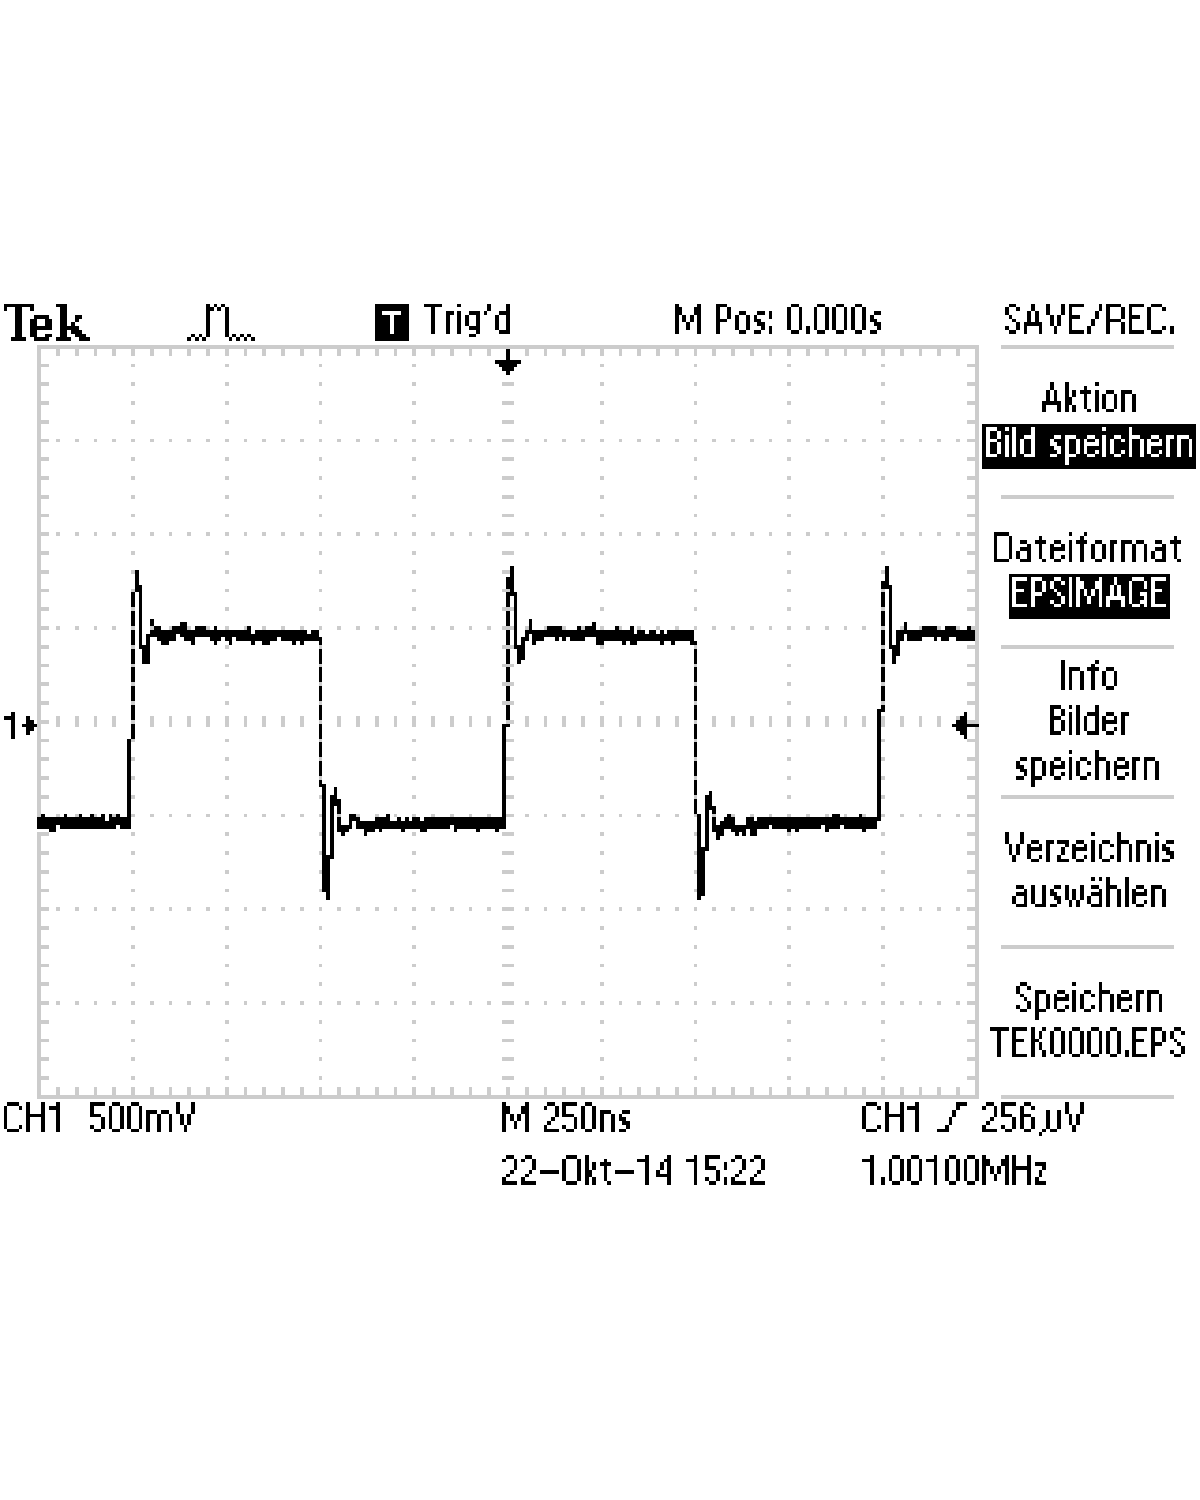
\includegraphics[scale = 0.5]{3_3.pdf}
  	\caption[Aufnahme des Signals bei 1MHz, mit einem Abschlusswiderstand von 50$\Omega$]{Aufnahme des Signals bei 1MHz, mit einem Abschlusswiderstand von 50$\Omega$}
  \label{fig:3_3}
\end{figure}

\subsubsection{Langes Koaxialkabel mit Kurzschluß am Ende}

Im vierten Versuchsteil sollte das Koaxialkabel mit einem Kurzschluss abgeschlossen werden. Dabei ergab sich auf dem Oszilloskop die Kurve in Abbildung \ref{fig:3_4}. Es fällt auf, dass das Signal stark verzerrt wurde, da das Signal mit umgekehrtem Vorzeichen reflektiert wurde.

\begin{figure}[H] 
  \centering
    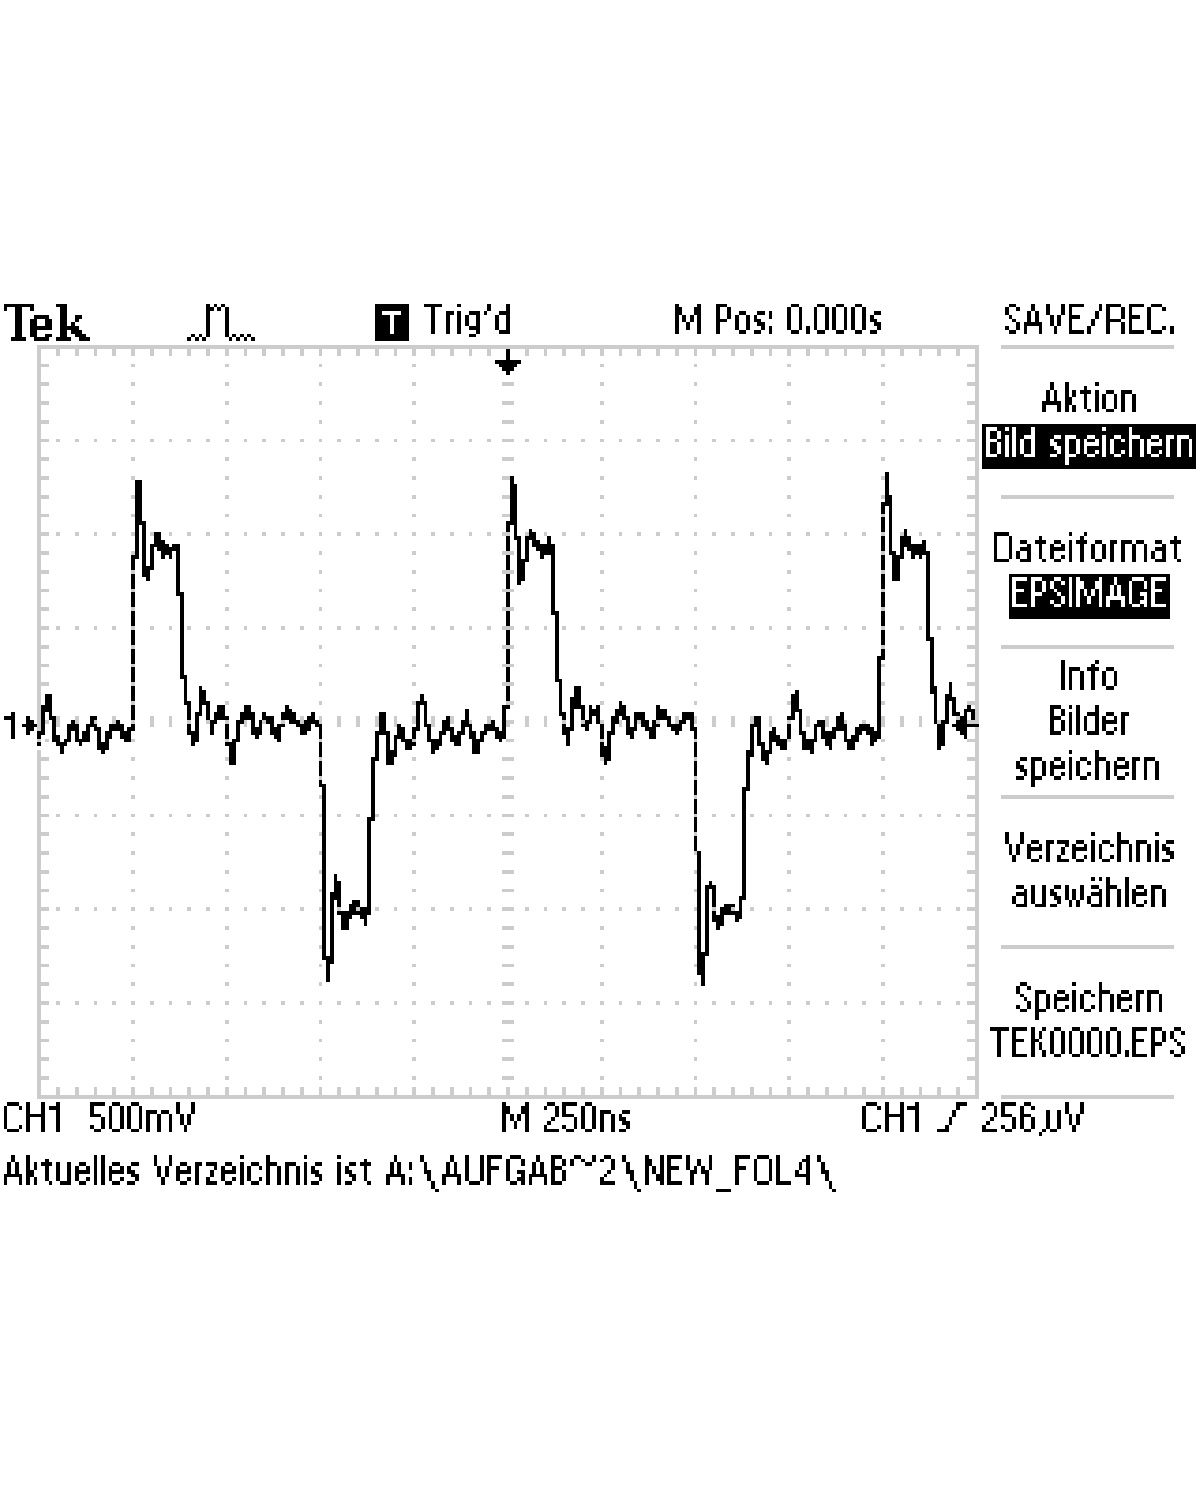
\includegraphics[trim = 0cm 6cm 0cm 0cm,clip , scale = 0.5]{3_4.pdf}
  	\caption[Aufnahme des Signals bei 1MHz, mit einem Kurzschluss am Ende]{Aufnahme des Signals bei 1MHz, mit einem Kurzschluss am Ende}
  \label{fig:3_4}
\end{figure}

\subsubsection{Langes Koaxialkabel mit variablem Abschlußwiderstand}

Im letztem Aufgabenteil sollte am Ende des Koaxialkabels ein Potentiometer angeschlossen werden und der Widerstand so eingestellt werden, dass das Rechtecksignal möglichst gut übertragen wird. Dabei wurde ein Wiederstandwert von 51,4$\Omega$ gemessen. Es ergab sich die Kurve in Abbildung \ref{fig:3_5}.

\begin{figure}[H] 
  \centering
    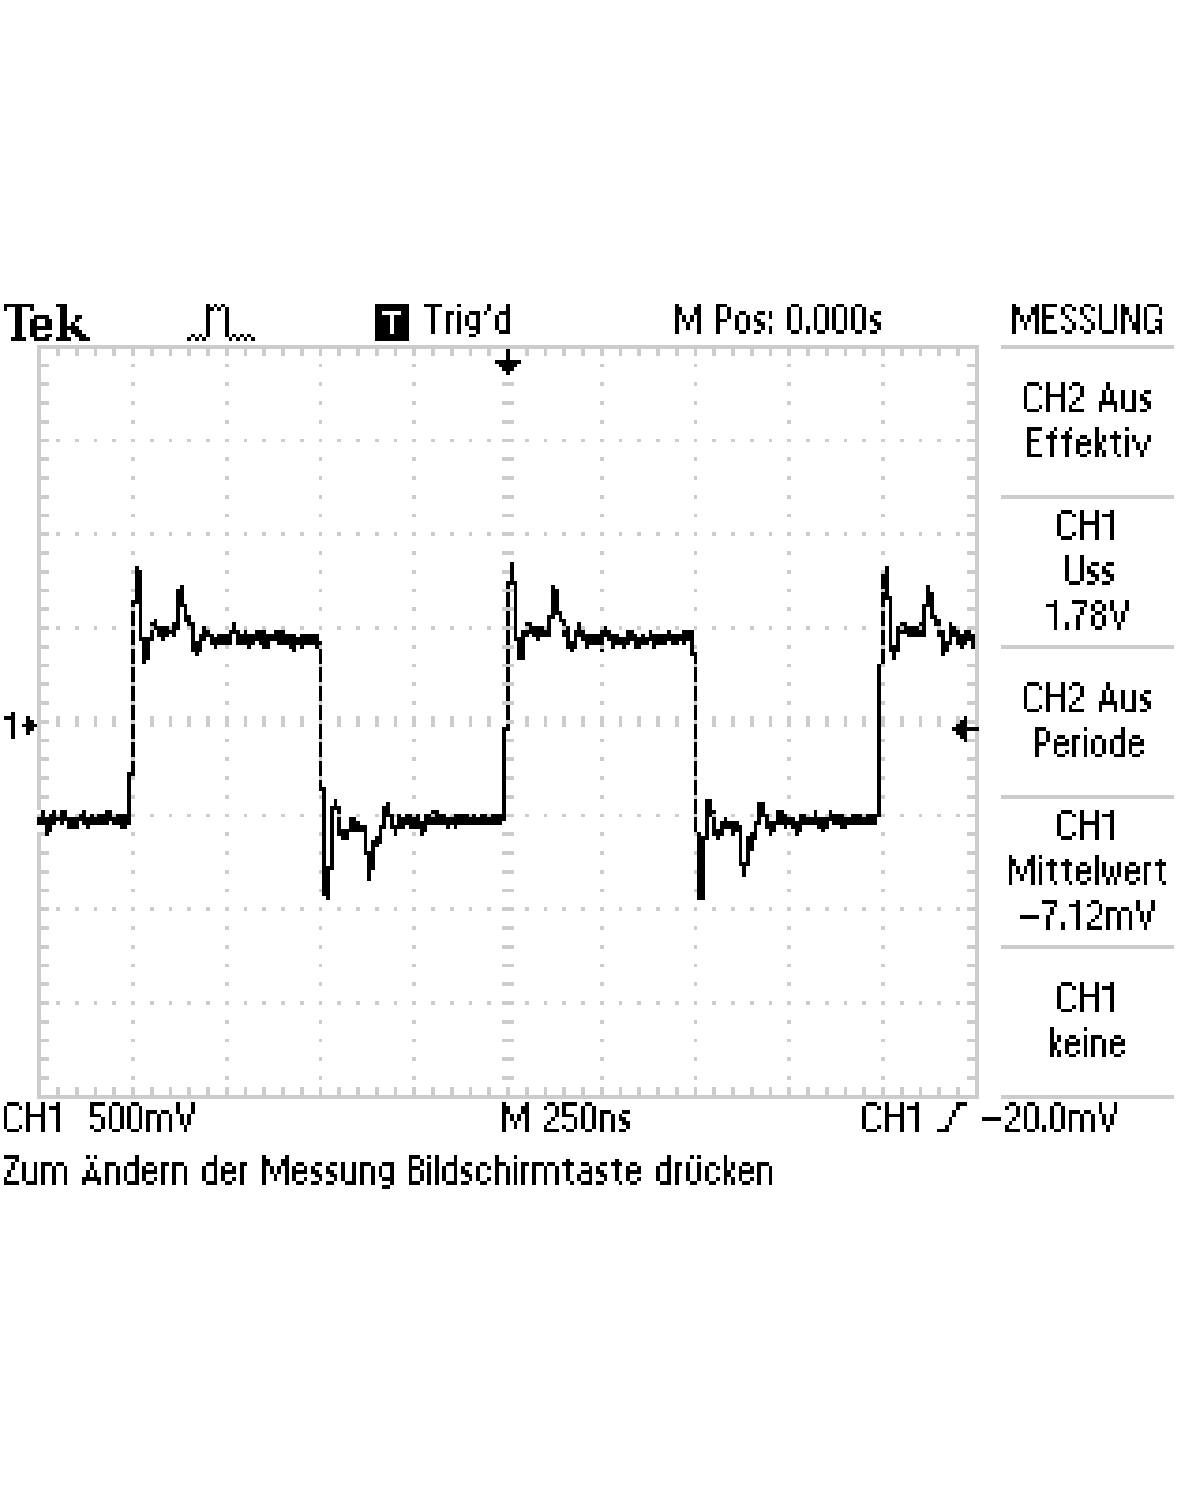
\includegraphics[trim = 0cm 6cm 0cm 0cm,clip , scale = 0.5]{3_5.pdf}
  	\caption[Aufnahme des Signals bei 1MHz, mit Potentiometer am Ende]{Aufnahme des Signals bei 1MHz, mit Potentiometer am Ende}
  \label{fig:3_5}
\end{figure}

\subsection{Diskussion}
%(immer) die gemessenen werte und die bestimmten werte über die messfehler mit literaturwerten oder untereinander vergleichen
%in welchem fehlerintervall des messwertes liegt der literaturwert oder der vergleichswert?
%wie ist der relative anteil des fehlers am messwert und damit die qualität unserer messung?
%in einem satz erklären, wie gut unser fehler und damit unsere messung ist
%kurz erläutern, wie systematische fehler unsere messung beeinflusst haben könnten
%(wichtig) zum schluss ansprechen, in wie weit die ergebnisse mit der theoretischen vorhersage übereinstimmen
%--------------------------------------------------------------------------------------------
%falls tabellen mit den messwerten zu lang werden, kann die section mit den messwerten auch hinter der diskussion angefügt bzw. eine section mit dem anhang eingefügt werden.

Die besseren Übertragungseigenschaften eines Koaxialkabels gegenüber dem Bananenkabel ließen sich durch die Messungen bestätigen. Auch die Reflexionseigenschaften des Koaxialkabels wurden vermessen. Die Signalgeschwindigkeit wurde mit \unit[(1,916 $\pm 0,02$ ) $\cdot 10^9$]{$\frac{\text{m}}{\text{s}}$} bestimmt, als Richtwert wurden in der Versuchsbeschreibung ca. \unit[2 $\cdot 10^9$]{$\frac{\text{m}}{\text{s}}$} angegeben. Der gemessene Wellenwiderstand wurde mit 51,4$\Omega$ gemessen erwartet wurde ein Wert von 51$\Omega$.




\section{Verdrillte Leitungen (Twisted Pair)}
%kurz das ziel dieses versuchsteiles ansprechen, damit keine zwei überschriften direkt übereinander stehen!
%bei schwierigeren versuchen kann auch der theoretische hintergrund erläutert werden. (mit formeln, herleitungen und erklärungen)

In diesem Versuchsabschnitt werden die Reflexionseigenschaften eines Patchkabels untersucht.

\subsection{Versuchsaufbau}
%skizze zum versuchsaufbau (oder foto) einfügen,   es muss erklärt werden wie das ganze funktioniert und welche speziellen einstellungen verwendet wurden (z.b. welche knöpfe an den geräten für die messung verdreht wurden)
Es werden zwei verschieden Aufbauten verwendet, wobei sich diese nur darin unterscheiden ob das Patchkabel am Ende offen oder mit einem Potentiometer abgeschlossen ist.

\subsubsection{Aufbau mit offenem Ende}

Im ersten Aufbau wird das Ende des Patchkabels offengelassen.

\begin{figure}[H] 
  \centering
    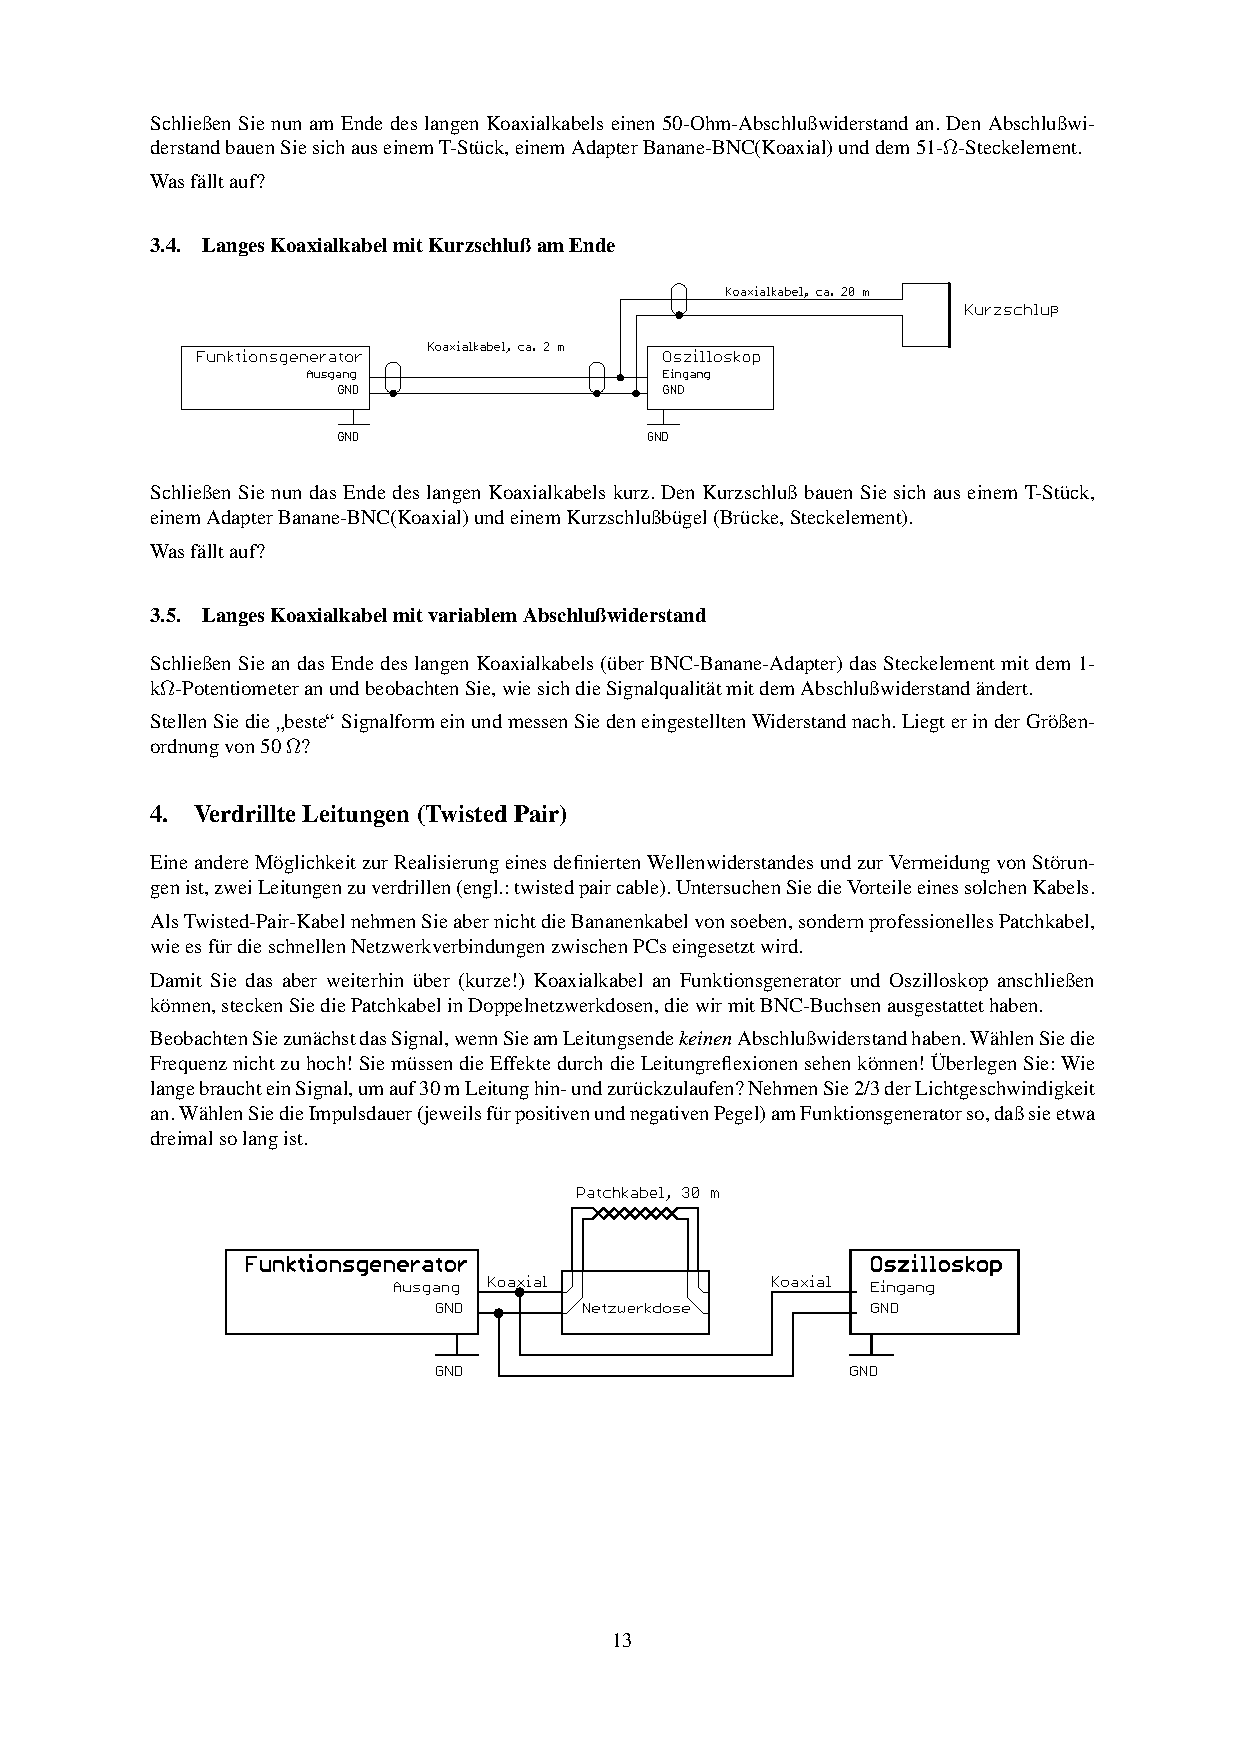
\includegraphics[trim = 10mm 60mm 10mm 200mm, clip, scale = 1]{3_4-4.pdf}
  	\caption[Schaltskizze einer Verbindung zwischen Funktionsgenerator und Oszilloskop, mit Patchkabel]{Schaltskizze einer Verbindung zwischen Funktionsgenerator und Oszilloskop, mit Patchkabel\footnotemark}
  \label{fig:4.1}
\end{figure}
\footnotetext{Abbildung entnommen von http://www.atlas.uni-wuppertal.de/$\sim$kind/ep1\_14.pdf Seite 14 am 19.10.2014}

\subsubsection{Aufbau mit Potentiometer am Ende}

Im zweitem Aufbau wird das Ende des Patchkabels mit einem 1k$\Omega$Potentiometer abgeschlossen.

\begin{figure}[H] 
  \centering
    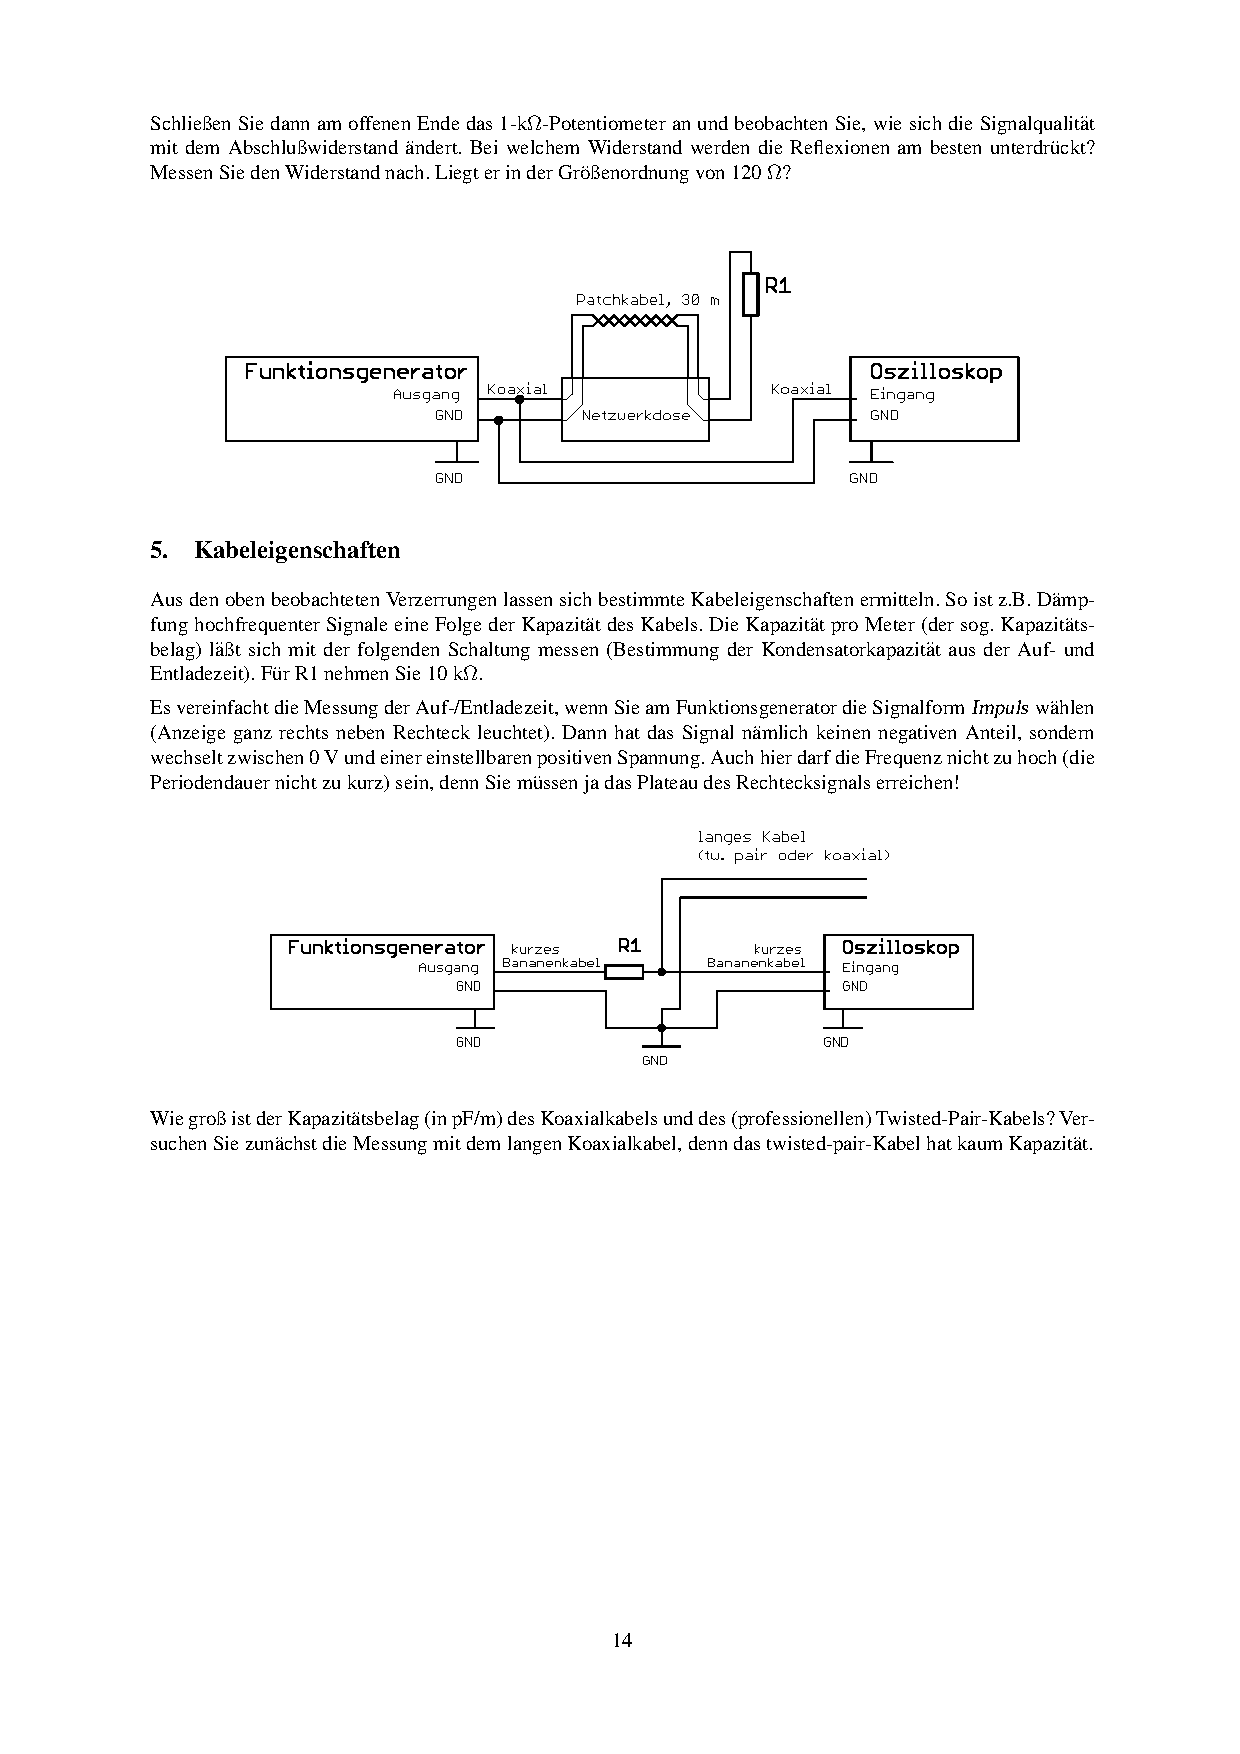
\includegraphics[trim = 10mm 210mm 10mm 40mm, clip, scale = 1]{4-5.pdf}
  	\caption[Schaltskizze einer Verbindung zwischen Funktionsgenerator und Oszilloskop, mit Patchkabel (geschlossen mit Potentiometer)]{Schaltskizze einer Verbindung zwischen Funktionsgenerator und Oszilloskop, mit Patchkabel (geschlossen mit Potentiometer)\footnotemark}
  \label{fig:4.2}
\end{figure}
\footnotetext{Abbildung entnommen von http://www.atlas.uni-wuppertal.de/$\sim$kind/ep1\_14.pdf Seite 14 am 19.10.2014}

\subsection{Versuchsdurchführung}
%erklären, !was! wir machen, !warum! wir das machen und mit welchem ziel
%(wichtig) präzize erklären, wie bei dem versuch vorgegangen und was gemacht wurde
In Aufgabe 4.1 wird analog zu Aufgabe 3.2 ein 30m langes Patchkabel über ein T-Stück angeschlossen (Länge vorgegeben). Die Laufzeit des am offenen Ende reflektierten Signals kann wieder über die Breite der Überlagerten rechten Flancke bestimmt werden (als Vergleichswert wurde eine Phasengeschwindigkeit von $\frac{2}{3}C_0$ angenommen).
In Aufgabe 4.2 wird wieder ein Potentiometer zur Bestimmung des Wellenwiderstandes angeschlossen.

\subsection{Verwendete Formeln}
%eine legende kann angefertigt werden, die selbstverständlichen buchstaben müssen nicht extra erklärt werden
%mit knappen erklärungen die !verwendeten! formeln, sowie die zugehörige fehlerrechnung einfügen.
Als Vergleichswert für die Durchlaufzeit $t$ ergibt sich unter der Annahme $v_{ph} = \frac{2}{3}C_0 = \sqrt{\frac{1}{\mu\epsilon}}$:
\begin{align}
t=\frac{2 L}{\frac{2}{3}C_0} \Rightarrow \frac{\unit[60]{m}}{\frac{2}{3}C_0} \cong \unit[300,21\cdot10^{-9}]{s}
\label{eqn:4}
\end{align}

\subsection{Auswertung}
%zuerst !alle! errechneten werte entweder in ganzen sätzen aufzählen, oder in tabellen (übersichtlicher) dargestellen, sowie auf die verwendeten formeln verweisen (die referenzierung der formel kann in der überschrift stehen)
%kurz erwähnen (vor der tabelle), warum wir das ganze ausrechnen bzw. was wir dort ausrechnen
%danach histogramme und plots erstellen, wobei wenn möglich funktionen durch die plots gelegt werden (zur not können auch splines benutzt werden, was aber angegeben werden muss)
%bei fits immer die funktion und das reduzierte chiquadrat mit angegeben, wobei auf verständlichkeit beim entziffern der zehnerpotenzen geachtet werden muss z.b. f(x)=(wert+-fehler)\cdot10^{irgendeine zahl}\cdot x + (wert+-fehler)\cdot10^{irgendeine zahl}
%bei jedem fit erklären, nach welchem zusammenhang gefittet wurde und warum!
%bei plots darauf achten, dass die achsenbeschriftung (auch die tics) die richtige größe haben und die legende im plot nicht die messwerte verdeckt
%kurz die aufgabenstellung abgehandeln

Es wurde das Signal bei offenem und mit einem Potentiometer abgeschlossenem Ende untersucht.

\subsubsection{Aufbau mit offenem Ende}

Auf der Aufnahme der Signalkurve des Oszilloskops, Abbildung \ref{fig:4_o} ist deutlich der Bereich zu sehen in dem das Signal noch durch das Patchkabel läuft. Dabei wurde eine Durchlaufzeit von \unit[296]{ns} gemessen. Nach Gleichung \ref{eqn:4} ergibt sich ein Theoriewert von 300ns.

\begin{figure}[H] 
  \centering
    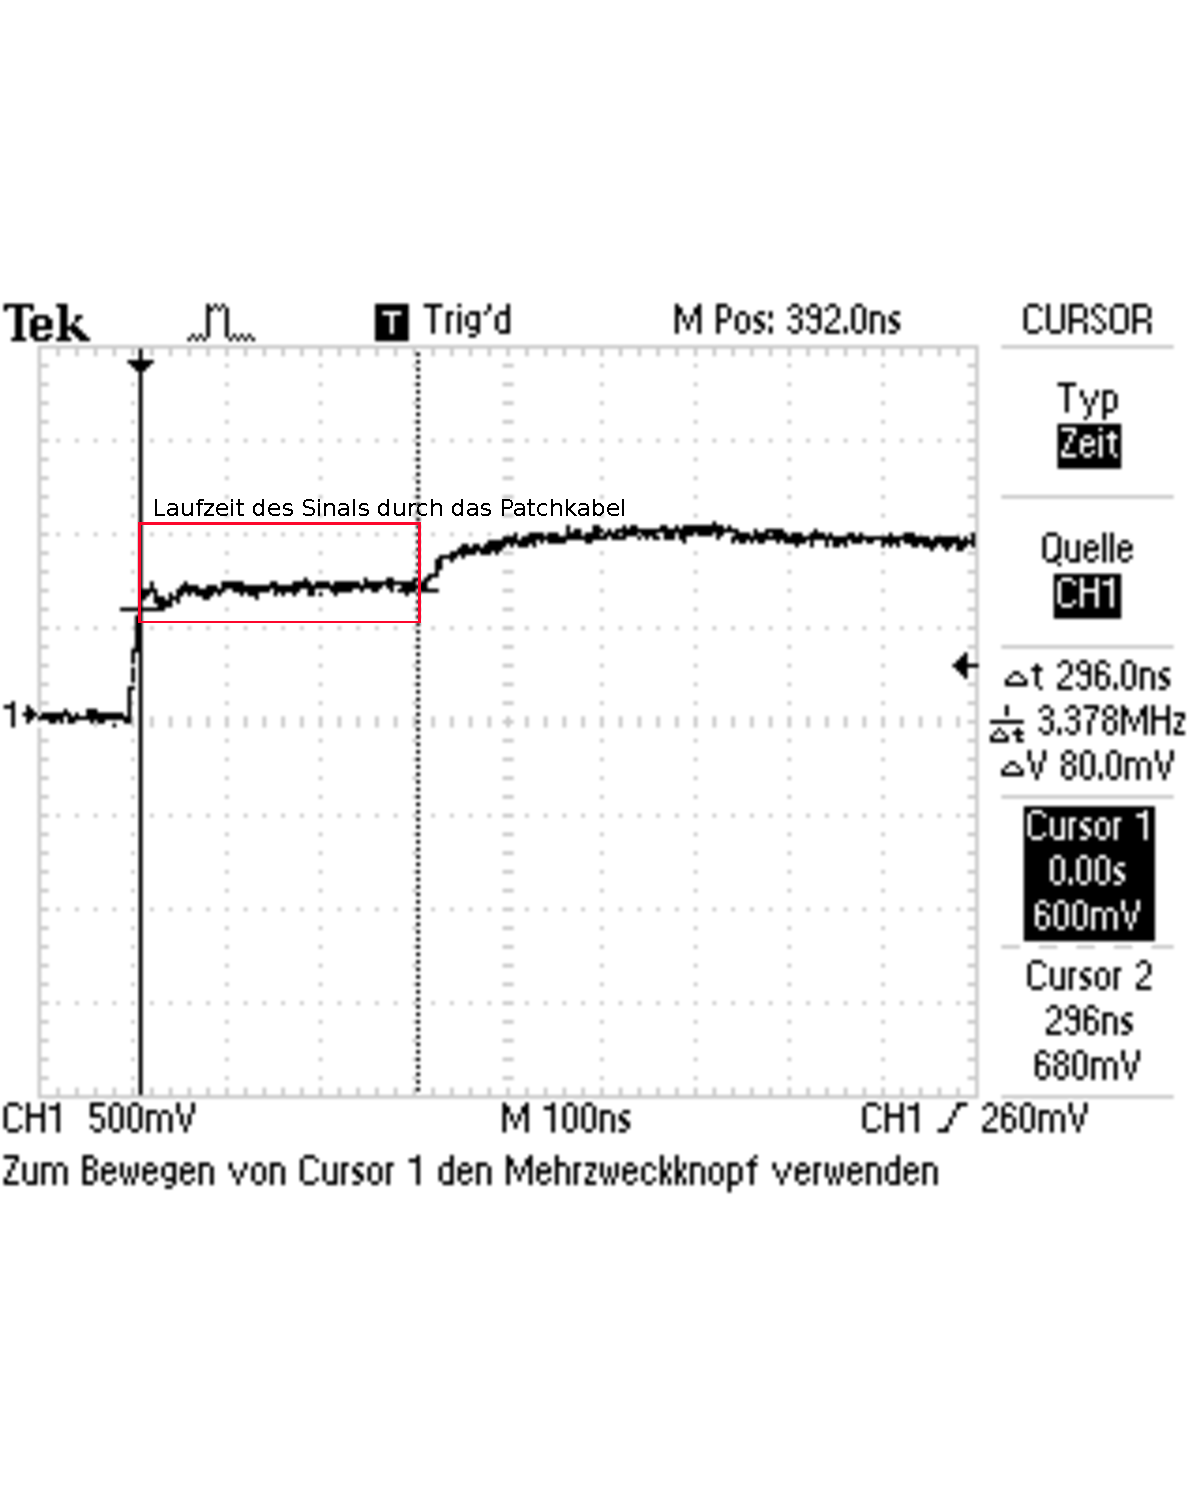
\includegraphics[scale = 0.5]{4_o.pdf}
  	\caption[Aufnahme des Signals, mit offenem Ende]{Aufnahme des Signals, mit offenem Ende}
  \label{fig:4_o}
\end{figure}

\subsubsection{Aufbau mit Potentiometer am Ende}

Im zweitem Versuchsteil war das Potentiometer so einzustellen, dass die Reflexion unterdrückt wird, dabei wurde das Potentiometer auf 118,7$\Omega$ eingestellt und es ergab sich auf dem Oszilloskop die Kurve aus Abbildung \ref{fig:4_a}.

\begin{figure}[H] 
  \centering
    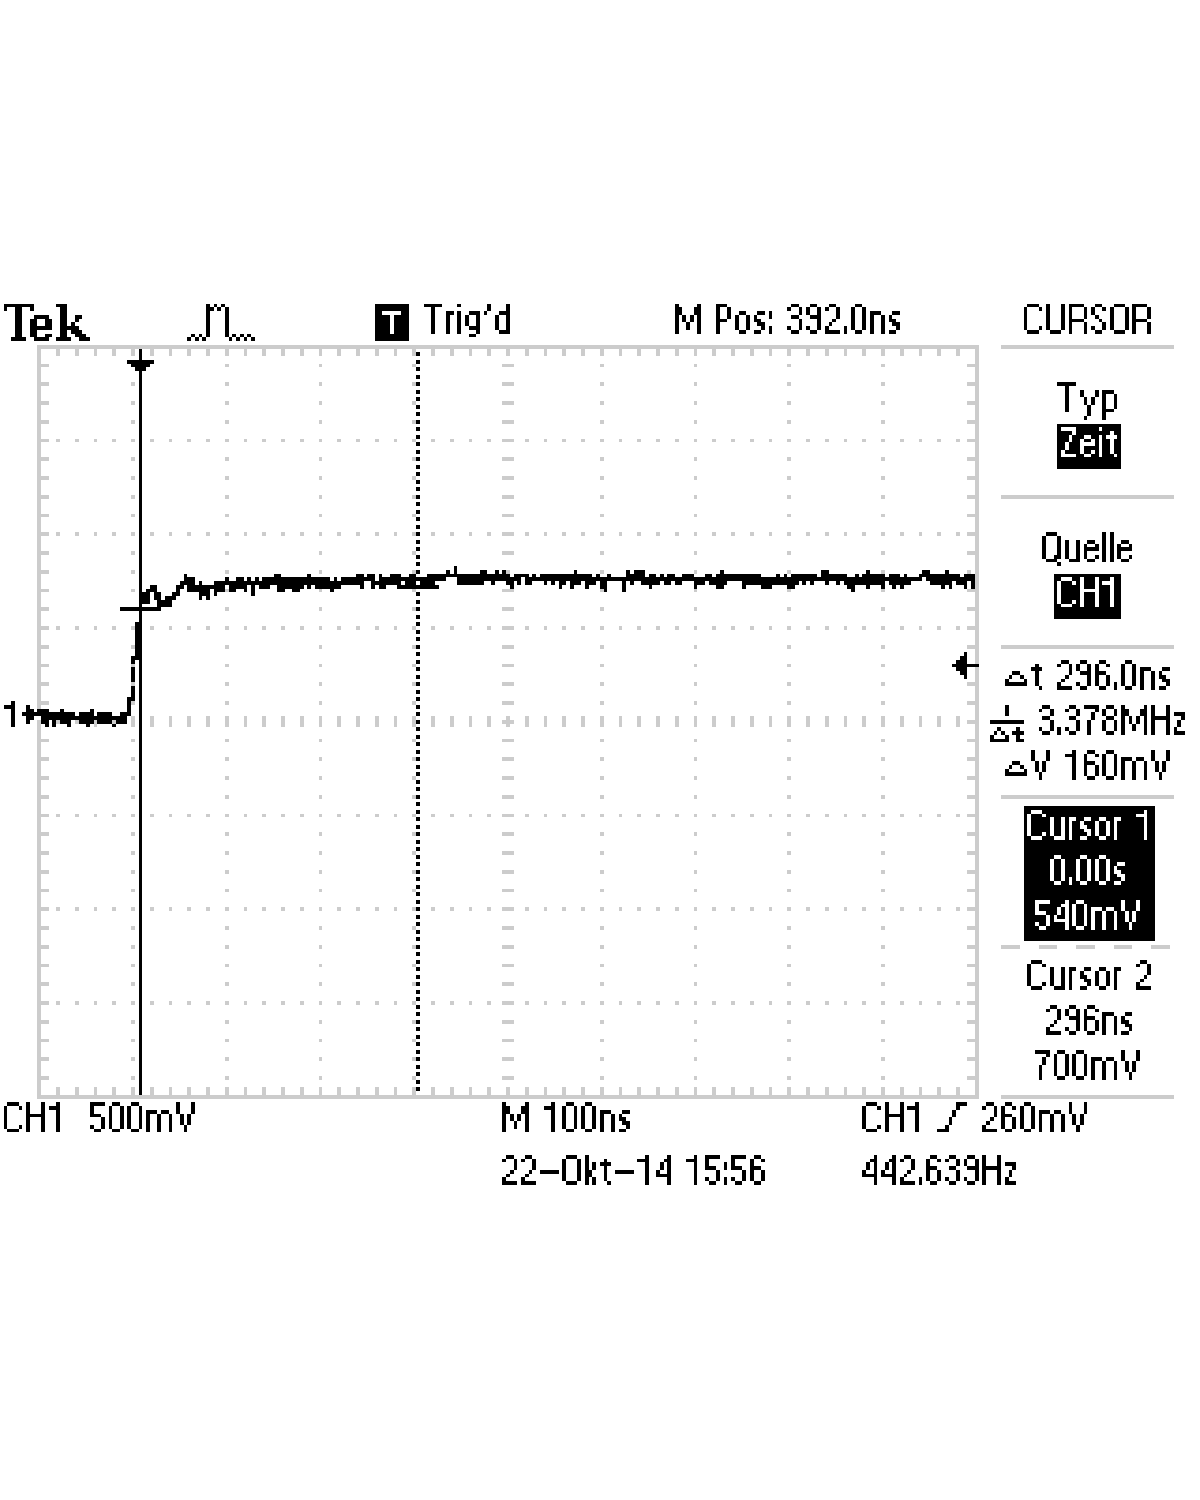
\includegraphics[scale = 0.5]{4_a.pdf}
  	\caption[Aufnahme des Signals, mit offenem Ende]{Aufnahme des Signals, mit Potentiometer Ende}
  \label{fig:4_a}
\end{figure}

\subsection{Diskussion}
%(immer) die gemessenen werte und die bestimmten werte über die messfehler mit literaturwerten oder untereinander vergleichen
%in welchem fehlerintervall des messwertes liegt der literaturwert oder der vergleichswert?
%wie ist der relative anteil des fehlers am messwert und damit die qualität unserer messung?
%in einem satz erklären, wie gut unser fehler und damit unsere messung ist
%kurz erläutern, wie systematische fehler unsere messung beeinflusst haben könnten
%(wichtig) zum schluss ansprechen, in wie weit die ergebnisse mit der theoretischen vorhersage übereinstimmen
%--------------------------------------------------------------------------------------------
%falls tabellen mit den messwerten zu lang werden, kann die section mit den messwerten auch hinter der diskussion angefügt bzw. eine section mit dem anhang eingefügt werden.


Im ersten Versuchsteil ist die Reflexion des Signals am offenen Ende des Kabels mit \unit[296]{ns} sehr nah am Theoriewert von \unit[300]{ns}. Im zweitem Versuchsteil wurde in der Versuchsanleitung\footnote{http://www.atlas.uni-wuppertal.de/$\sim$kind/ep1\_14.pdf Seite 14 am 23.10.2014} ein Wellenwiderstand von 120$\Omega$ angegeben, der gemessene Wert liegt bei 118,4$\Omega$, was ein guter Wert ist.


\section{Kabeleigenschaften}
%kurz das ziel dieses versuchsteiles ansprechen, damit keine zwei überschriften direkt übereinander stehen!
%bei schwierigeren versuchen kann auch der theoretische hintergrund erläutert werden. (mit formeln, herleitungen und erklärungen)

In diesem Versuchsabschnitt werden die Kabeleigenschaften des Kapazitätsbelags untersucht.

\subsection{Versuchsaufbau}
%skizze zum versuchsaufbau (oder foto) einfügen,   es muss erklärt werden wie das ganze funktioniert und welche speziellen einstellungen verwendet wurden (z.b. welche knöpfe an den geräten für die messung verdreht wurden)

\begin{figure}[H] 
  \centering
    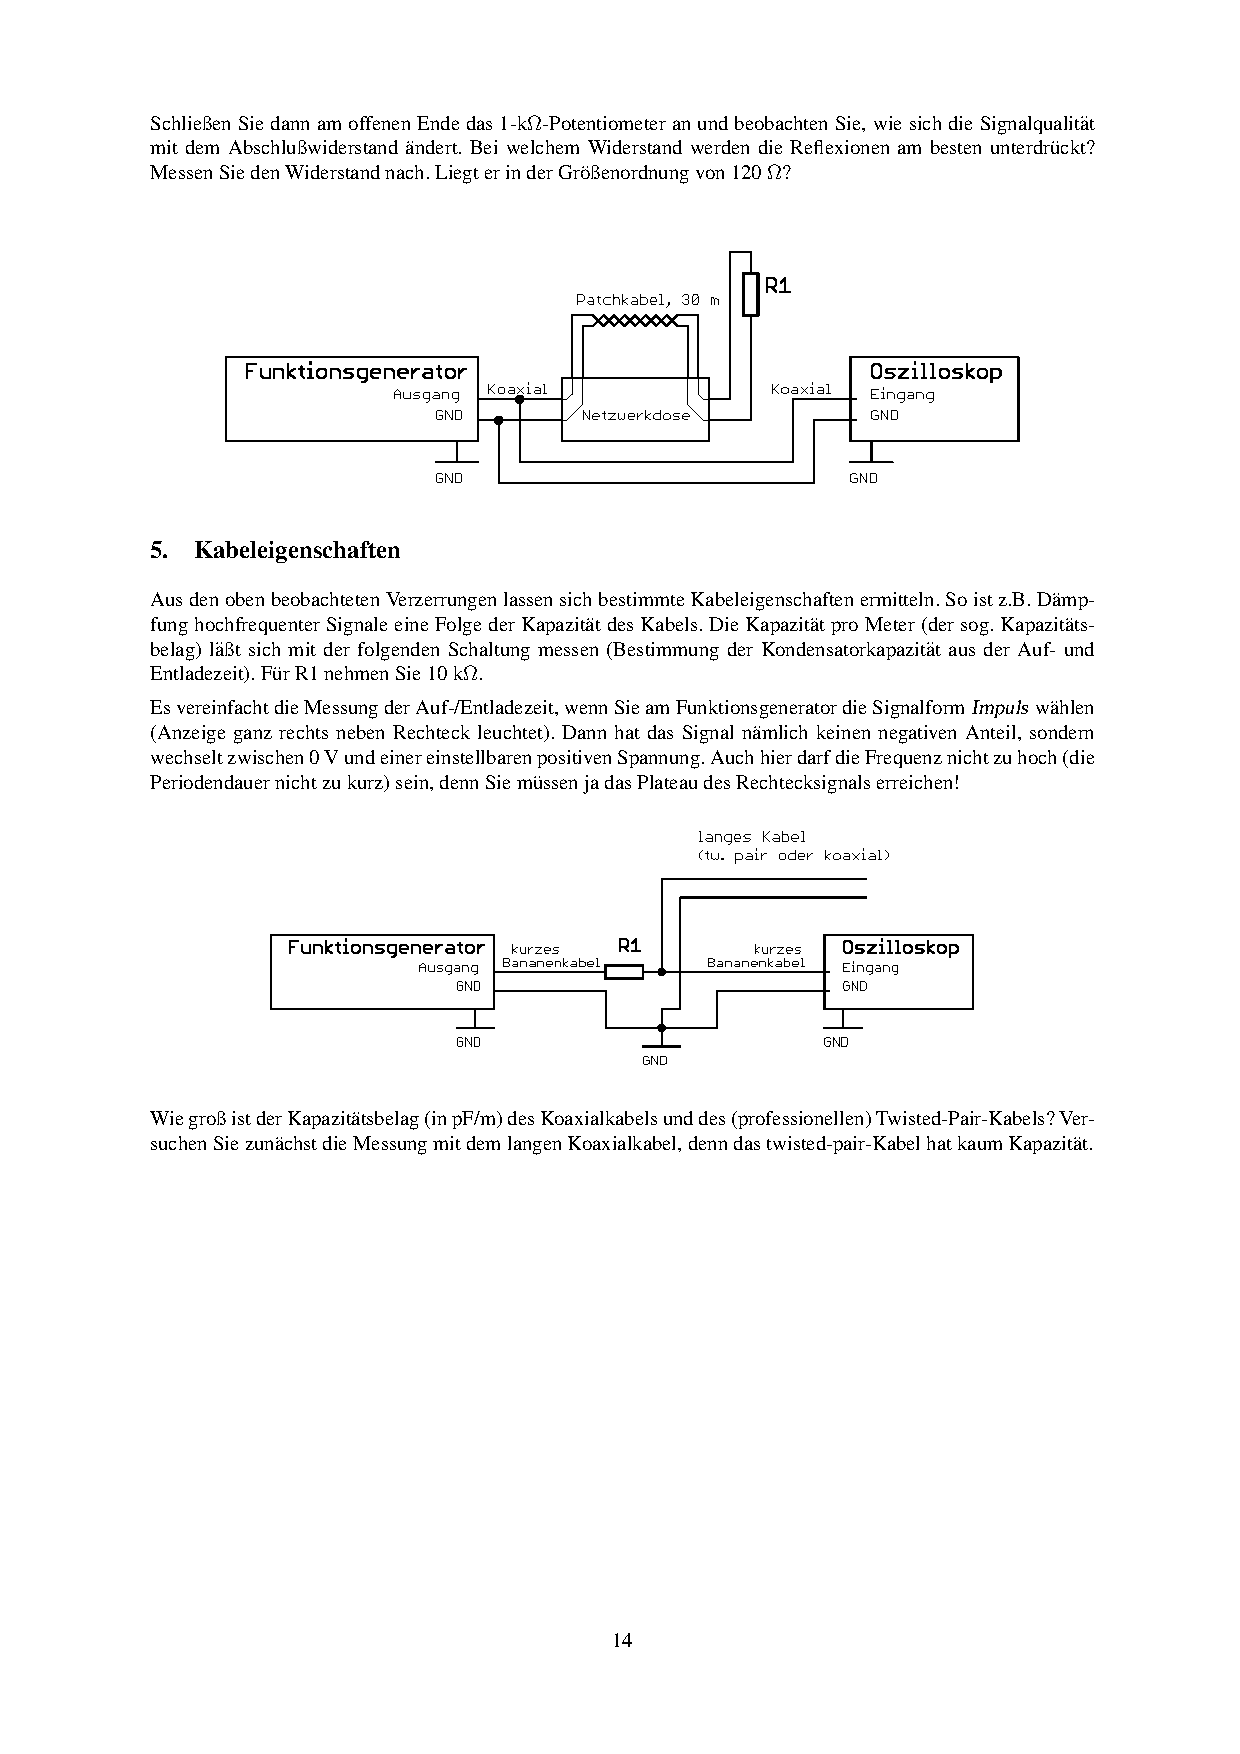
\includegraphics[trim = 10mm 110mm 10mm 140mm, clip, scale = 1]{4-5.pdf}
  	\caption[Schaltskizze zur Bestimmung des Kapazitätsbelags]{Schaltskizze zur Bestimmung des Kapazitätsbelags\footnotemark}
  \label{fig:5}
\end{figure}
\footnotetext{Abbildung entnommen von http://www.atlas.uni-wuppertal.de/$\sim$kind/ep1\_14.pdf Seite 14 am 19.10.2014}


\subsection{Versuchsdurchführung}
%erklären, !was! wir machen, !warum! wir das machen und mit welchem ziel
%(wichtig) präzize erklären, wie bei dem versuch vorgegangen und was gemacht wurde
In der 5. Aufgabe soll der sogenannte Kapazitätsbelag des Koaxialkabels bestimmt werden. Damit die Aufladezeiten nicht zu kurz werden, wird ein \unit[10]{k$\Omega$} Widerstand davorgeschaltet. Aus der Halbwertszeit des Auf- bzw. Entladevorgangs oder besser aus dem Mittelwert kann dann die Kapazität des Kabels und damit auch der Kapazitätsbelag bestimmt werden.
\subsection{Verwendete Formeln}
%eine legende kann angefertigt werden, die selbstverständlichen buchstaben müssen nicht extra erklärt werden
%mit knappen erklärungen die !verwendeten! formeln, sowie die zugehörige fehlerrechnung einfügen.
Aus der Dgl. für die Kondensatorauflade- bzw. Kondensatorentladezeit ergibt sich der Zusammenhang für den Kapazitätsbelag $\kappa$:
\begin{align}
 \kappa = \frac{\tau}{L \ln(2) R}
 \label{eqn:5}
\end{align}
$\tau$ die Halbwertszeit, L die Länge des Kabels und R der Vorwiderstand. Es wird wie üblich Gaußsche Fehlerfortpflanzung verwendet.
\subsection{Auswertung}
%zuerst !alle! errechneten werte entweder in ganzen sätzen aufzählen, oder in tabellen (übersichtlicher) dargestellen, sowie auf die verwendeten formeln verweisen (die referenzierung der formel kann in der überschrift stehen)
%kurz erwähnen (vor der tabelle), warum wir das ganze ausrechnen bzw. was wir dort ausrechnen
%danach histogramme und plots erstellen, wobei wenn möglich funktionen durch die plots gelegt werden (zur not können auch splines benutzt werden, was aber angegeben werden muss)
%bei fits immer die funktion und das reduzierte chiquadrat mit angegeben, wobei auf verständlichkeit beim entziffern der zehnerpotenzen geachtet werden muss z.b. f(x)=(wert+-fehler)\cdot10^{irgendeine zahl}\cdot x + (wert+-fehler)\cdot10^{irgendeine zahl}
%bei jedem fit erklären, nach welchem zusammenhang gefittet wurde und warum!
%bei plots darauf achten, dass die achsenbeschriftung (auch die tics) die richtige größe haben und die legende im plot nicht die messwerte verdeckt
%kurz die aufgabenstellung abgehandeln

Im letztem Versuchsteil sollte der Kapazitätsbelag eines Koaxialkabels und eines Patchkabels bestimmt werden.
Dazu wurden die Auf- und Entladezeiten (Halbwertszeit) gemessen und daraus nach Gleichung \ref{eqn:5} die Kapazität bestimmt.
Der Widerstand betrug in beiden Aufbauten 10k$\Omega$ mit einem Fehler von 1\%, das Koaxialkabel war \unit[(11,5 $\pm 0,5$)]{m} lang und das Patchkabel \unit[30]{m}. Für das Patchkabel wurde eine Halbwertszeit von \unit[(10,4 $\pm 0,1$)]{ms} beim Aufladen und \unit[(11,5 $\pm 0,1$)]{ms} beim entladen gemessen, gemittelt ergibt sich ein Wert von \unit[(10,95 $\pm 0,1$)]{ms}, Abbildung \ref{fig:5_1}. Beim Koaxialkabel wurde eine Halbwertszeit von \unit[(9,2 $\pm 0,1$)]{ms} beim aufladen und \unit[(8,8 $\pm 0,1$)]{ms} beim entladen gemessen, es ergibt sich ein Mittelwert von \unit[(9 $\pm 0,1$)]{ms}, Abbildung \ref{fig:5_2}.
Für das Koaxialkabel ergibt sich für den Kapazitätsbelag ein Wert von \unit[(1,37 $\pm 0,01$) $10^{-7}$]{$\frac{\text{F}}{\text{m}}$}, für das Patchkabel ergibt sich ein Wert von \unit[(4,3 $\pm 0,1$) $10^{-8}$]{$\frac{\text{F}}{\text{m}}$}.

\begin{figure}[H] 
  \centering
    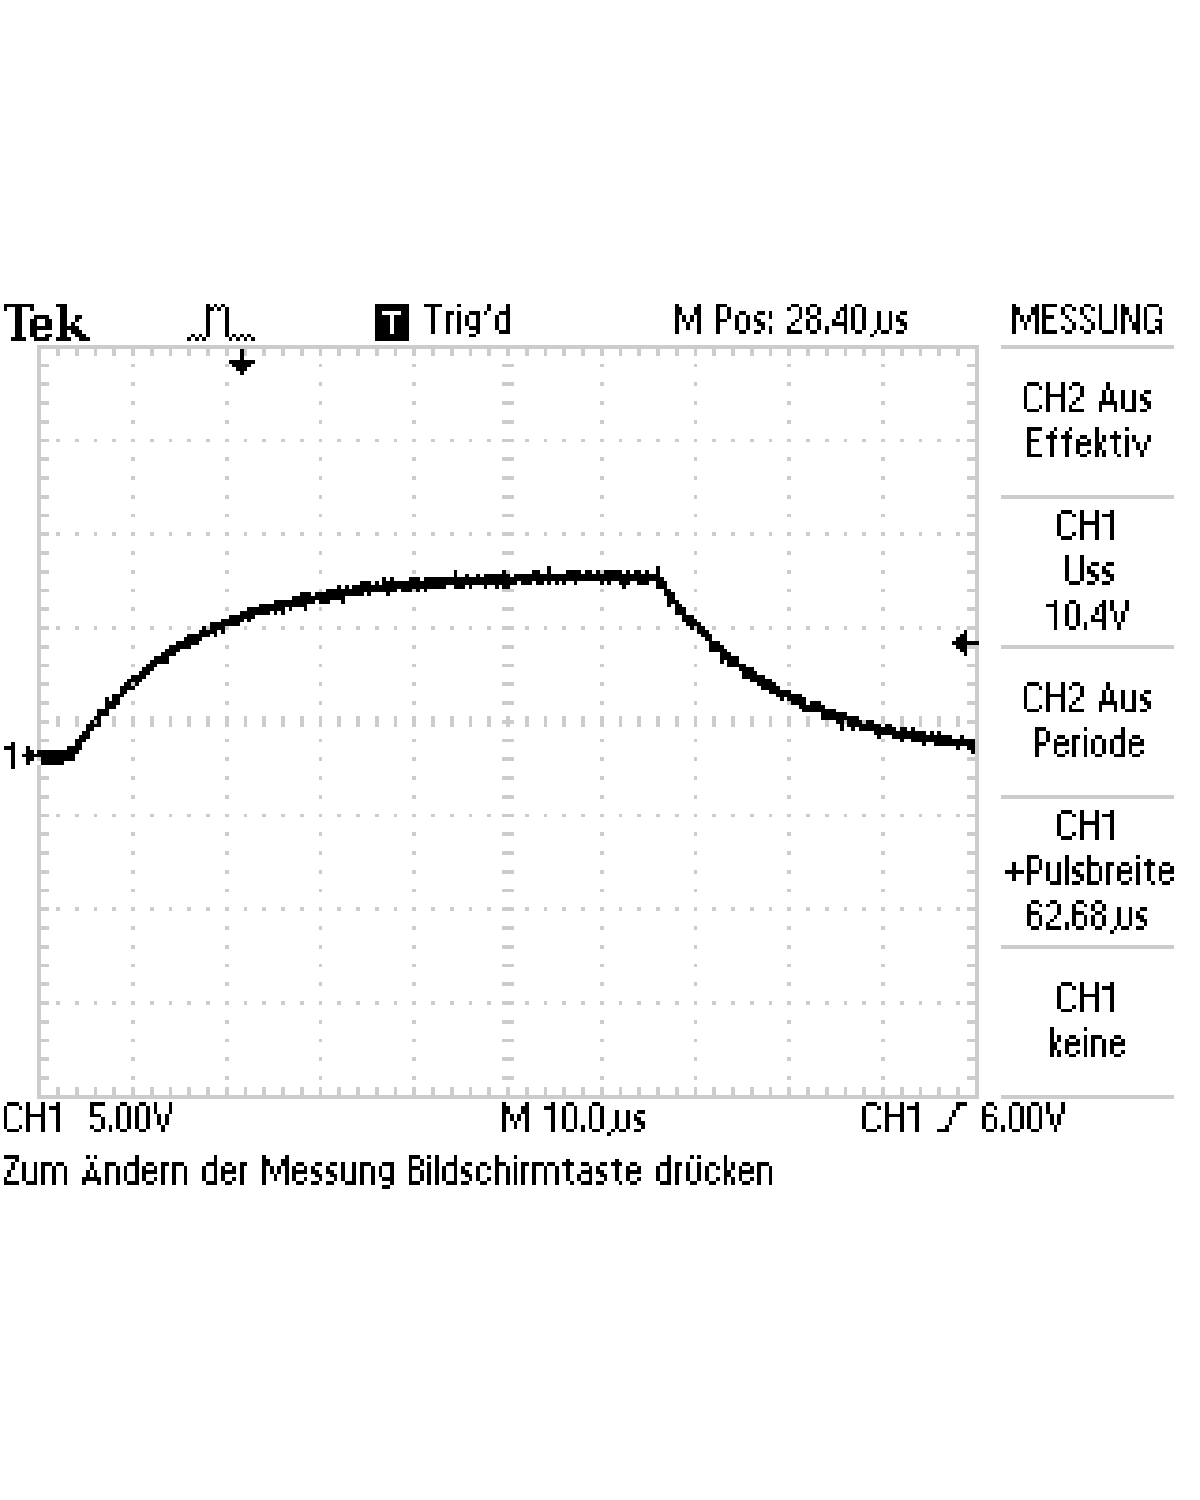
\includegraphics[scale = 0.5]{5_1.pdf}
  	\caption[Aufnahme des Signals für das Koaxialkabel]{Aufnahme des Signals für das Koaxialkabel}
  \label{fig:5_1}
\end{figure}


\begin{figure}[H] 
  \centering
    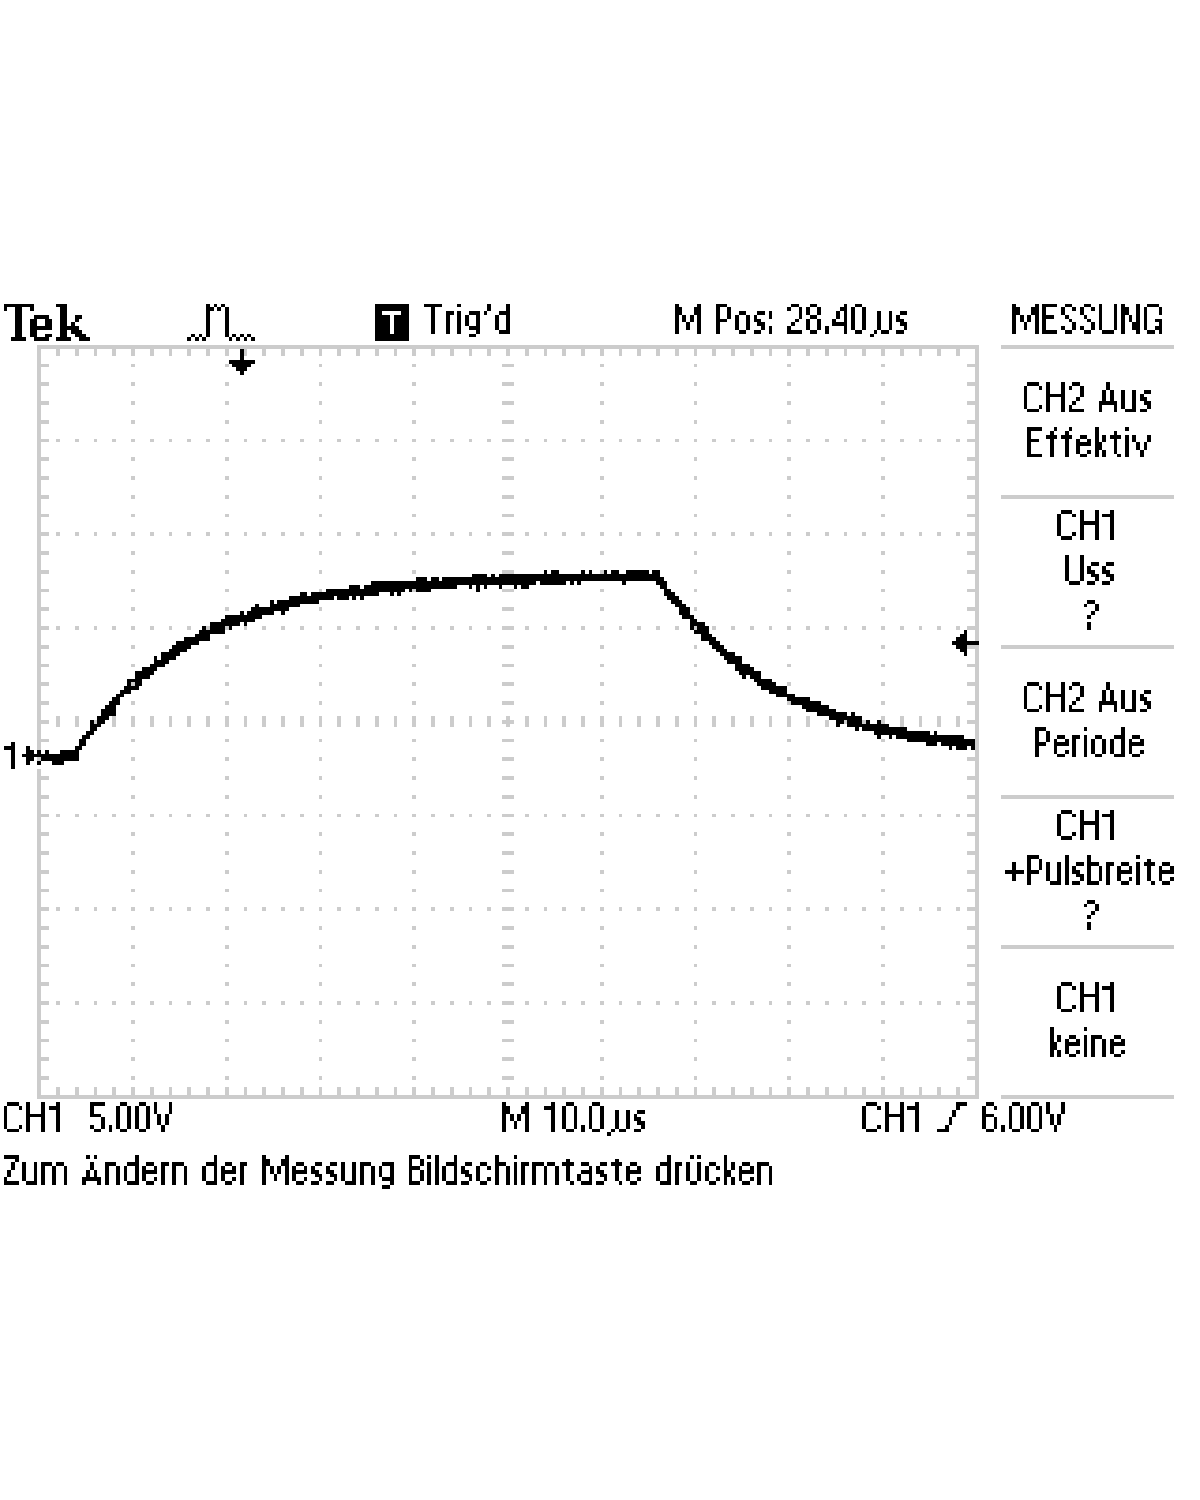
\includegraphics[scale = 0.5]{5_2.pdf}
  	\caption[Aufnahme des Signals für das Patchkabel]{Aufnahme des Signals für das Patchkabel}
  \label{fig:5_2}
\end{figure}


\subsection{Diskussion}
%(immer) die gemessenen werte und die bestimmten werte über die messfehler mit literaturwerten oder untereinander vergleichen
%in welchem fehlerintervall des messwertes liegt der literaturwert oder der vergleichswert?
%wie ist der relative anteil des fehlers am messwert und damit die qualität unserer messung?
%in einem satz erklären, wie gut unser fehler und damit unsere messung ist
%kurz erläutern, wie systematische fehler unsere messung beeinflusst haben könnten
%(wichtig) zum schluss ansprechen, in wie weit die ergebnisse mit der theoretischen vorhersage übereinstimmen
%--------------------------------------------------------------------------------------------
%falls tabellen mit den messwerten zu lang werden, kann die section mit den messwerten auch hinter der diskussion angefügt bzw. eine section mit dem anhang eingefügt werden.

Wie erwartet war der bestimmte Kapazitätsbelag für das Patchkabel geringer als für das Koaxialkabel.


\section{Fazit}
%im fazit nochmal alles zusammenfassen und den verlauf der messung abschätzen
%gravierende sytematische probleme bei den messungen nochmal betonen und die wertigkeit unserer ergebnisse einordnen

\end{document}

